\documentclass[a4paper,twoside,12pt,papersize, dvipdfmx]{iirthesis}
\usepackage{amsmath,amssymb,amsthm}
\usepackage{graphicx}
\usepackage{subcaption}
\usepackage{url}
\usepackage{otf}
\usepackage{minitoc}
\usepackage{bm}
\usepackage{amsmath,amssymb}
\usepackage{multirow}
\usepackage{times} % times new roman
\usepackage{pdfpages}
\usepackage{algorithmic}
\usepackage{algorithm}

% 単体コンパイルを可能にするための仕込み
\newcommand{\ifdraft}{false}

\newcommand{\figref}[1]{\figurename\ref{#1}}
\newcommand{\tabref}[1]{\tablename\ref{#1}}
\renewcommand{\eqref}[1]{式~(\ref{#1})}
\newcommand{\chapref}[1]{\ref{#1}章}
\newcommand{\secref}[1]{\ref{#1}節}
\newcommand{\ssecref}[1]{\ref{#1}項}
\newcommand{\appref}[1]{付録\ref{#1}}
\newcommand{\algoref}[1]{Algorithm.\ref{#1}}

\begin{document}
%\includepdf[pages=-]{title.pdf}

 \pagestyle{empty}		%ページ番号を消す
 \thesistype{{令和4年度 ポートフォリオ}}
 \title{\Huge{平面内センサレスin-handケージングマニピュレーションの計画}}
 \etitle{}
 \author{}
 \eauthor{}
 \miscinfo{
 \begin{tabular}{c}
 \\
 \vspace{-3mm}
 {\Large 2023年1月24日} \\[3em]
 {\Large 指導教員 : 前田 雄介 教授} \\[2em]
 {\Large 横浜国立大学 大学院 理工学府} \\
 {\Large 機械・材料・海洋系工学専攻} \\
 {\Large 機械工学教育分野} \\
 {\Large 21NA140 中西 佑太} \\
 \end{tabular}
 }
 \maketitle

\pagestyle{empty}
\cleardoublepage
\begin{center}
    \vspace{12em}
    \Large
{\sffamily \bfseries \huge{Planning of Planar Sensorless In-hand Caging Manipulation}}\\
    \vspace{2em}
    {\LARGE by}\\
    \vspace{2em}
    {\LARGE 21NA140 Yuta NAKANISHI}\\
    \vspace{9em}
    Supervisor: Professor Yusuke MAEDA\\
    \vspace{2em}
    A Master's Portfolio\\
    Submitted to\\
    the Specialization of Mechanical Engineering\\
    in the Department of Mechanical Engineering, Materials Science, and Ocean Engineering\\
    the Graduate School of Engineering Science of\\
    Yokohama National University\\
    \vspace{3em}
    January 24, 2023
\end{center}

\cleardoublepage	%奇数ページから始まるように改ページ

\frontmatter
\pagestyle{headings}	%ヘッダにページ番号,章・節番号,見出しを表示
%\setcounter{tocdepth}{2}
\dominitoc
\tableofcontents


\mainmatter
%語句の統一に関する注意書き
%〇コンフィギュレーション空間   ×コンフィグレーション空間
%〇対象物             ×物体
%〇位置・姿勢$\phi$                               ×位置・姿勢$\theta$
%〇目標位置・姿勢         ×ゴール位置・姿勢
%探索アルゴリズムに関する説明では「ゴール」を使う


% 黒魔術
\expandafter\ifx\csname ifdraft\endcsname\relax
    \documentclass[a4paper,twoside,12pt,papersize, dvipdfmx]{iirthesis}
    \usepackage{amsmath,amssymb,amsthm}
    \usepackage{graphicx}
    \usepackage{subcaption}
    \usepackage{url}
    \usepackage{otf}
    \usepackage{minitoc}
    \usepackage{bm}
    \usepackage{amsmath,amssymb}
    \begin{document}

    \newcommand{\figref}[1]{\figurename\ref{#1}}
    \newcommand{\tabref}[1]{\tablename\ref{#1}}
    \renewcommand{\eqref}[1]{式~(\ref{#1})}
    \newcommand{\chapref}[1]{\ref{#1}章}
    \newcommand{\secref}[1]{\ref{#1}節}
    \newcommand{\ssecref}[1]{\ref{#1}項}
    \newcommand{\appref}[1]{付録\ref{#1}}
\fi


\chapter{序論}\label{chap::intro}
\minitoc

\section{研究背景}\label{sec::intro::background}
近年,ロボット技術は飛躍的に進歩し,様々な産業に対してロボットの導入が進んでいる.このようなロボットに期待されていることの一つは,人間が行っている作業を代替することである.人間が行う作業は様々あるが,その一つに「In-handマニピュレーション」と呼ばれるものがある.これは,\figref{fig::intro::ihm}のように手の中で物体の位置・姿勢を変化させる動作のことである.このIn-handマニピュレーションをロボットハンドで再現しようとした研究は様々ある.現状,それらの研究の多くは力情報や位置情報を必要とし,マニピュレーション中のセンシングが不可欠となっている.\par

ところで,対象物の拘束手法の一つにケージング\cite{rimon1999}というものがある.これは,対象物の形状情報を基に,ロボットによる幾何学的な囲い込みで対象物を拘束する手法である.通常,対象物を拘束する際は力のつり合い条件等を考慮する必要があり,モデルが複雑になるとともに力覚センサが必要となる.一方,この手法では,ロボットの位置制御のみで実現可能なのでモデルが単純かつセンサを必要としない.\par

ケージングを用いることで,センサを使わないIn-handマニピュレーションを実現できる.具体的には,ロボットハンドで対象物をケージングにより拘束した後,囲いの形状を変化させていくことで,対象物の位置・姿勢(傾き)を操ることができる.\cite{komiyama2021}では,これを「センサレスin-handケージングマニピュレーション」と定義している.センサを使わないため安価にシステムを構築でき,またロボットハンドの位置情報のみを取り扱うのでシンプルな制御で事足りる.\par

本手法の,位置・姿勢(傾き)にばらつきのある対象物を特定の位置・姿勢に整列できるという特徴を踏まえて,パーツフィーダとしての実用化を目指している.後述するが,本手法では多様な形状の対象物をマニピュレーションできるので,多品種少量生産傾向にある昨今に有用なパーツフィーダになると考えている.

\begin{figure}[b]
\centering
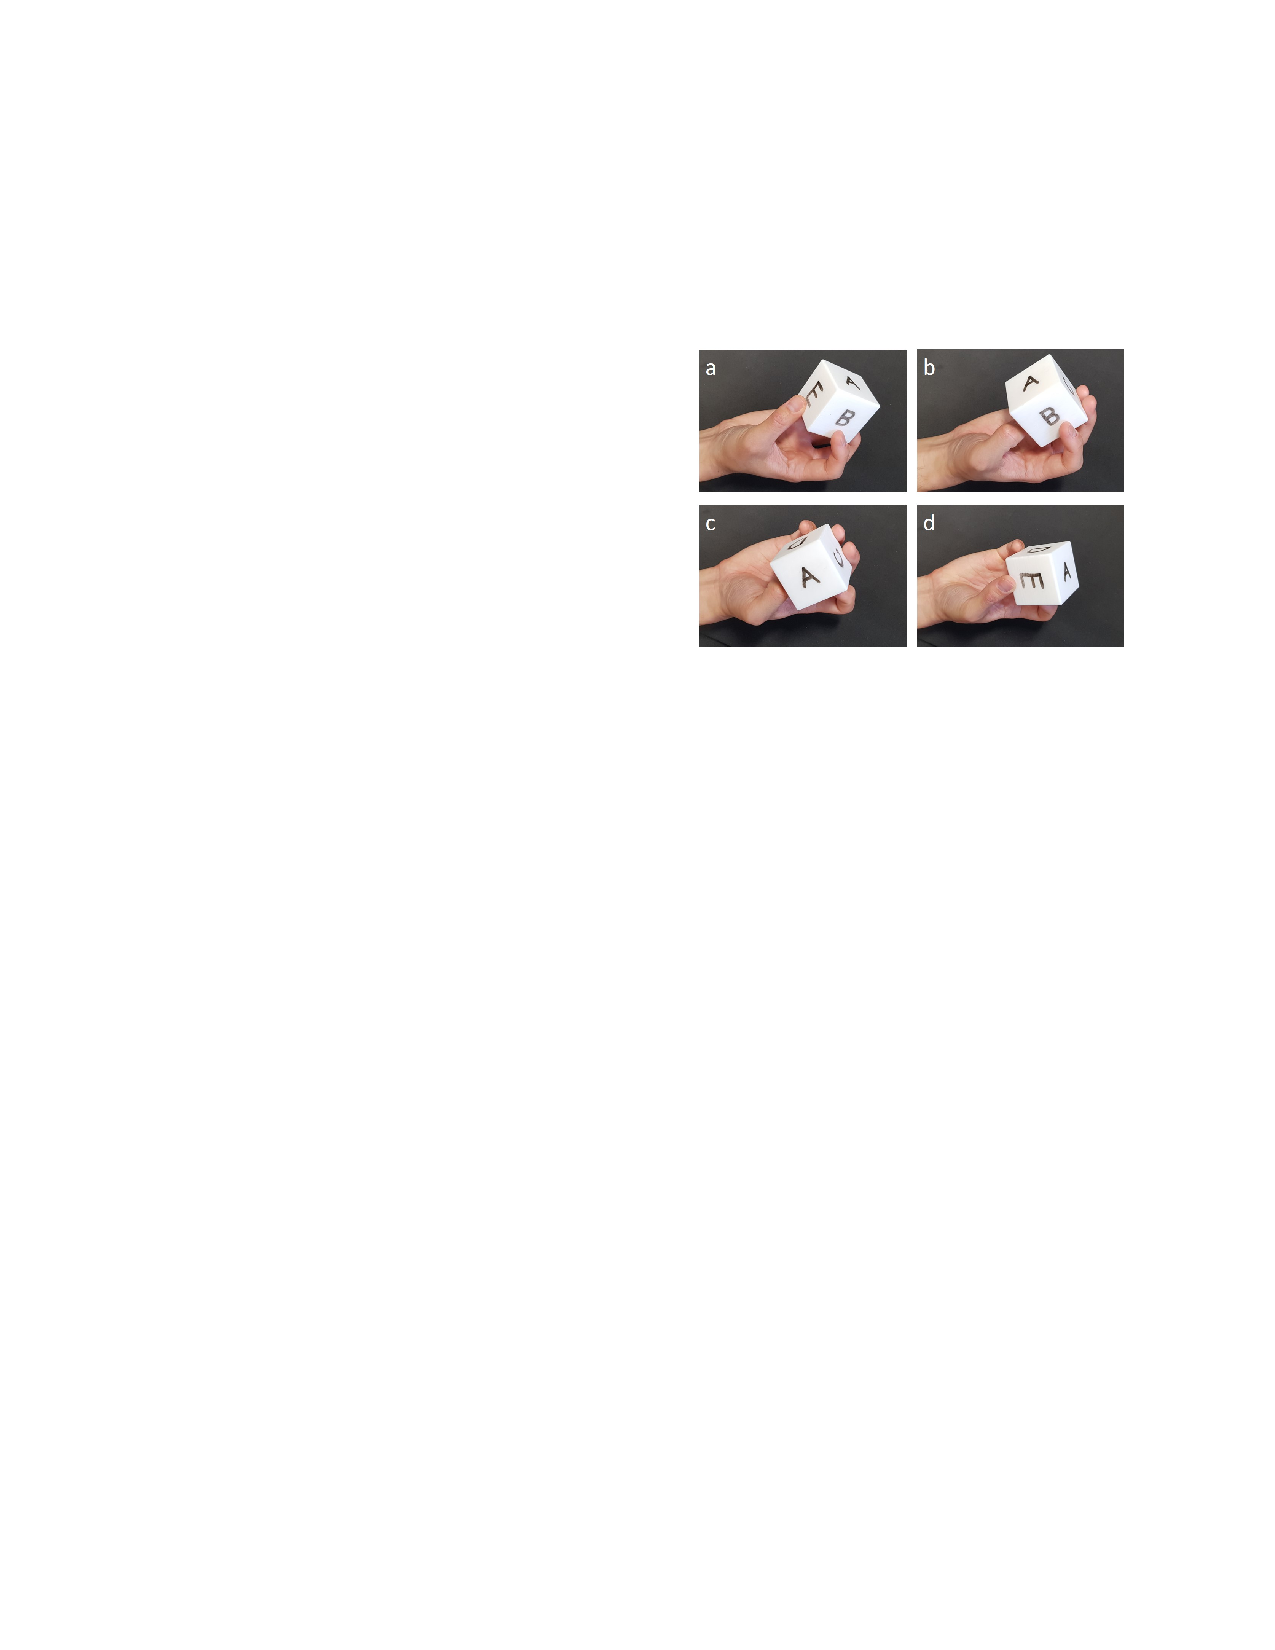
\includegraphics[width=0.35\hsize]{fig/1-introduction/Liarokapis2018_finger.pdf}
\caption{In-hand manipulation task with a 3D printed cube \cite{dwivedi2018}}
\label{fig::intro::ihm}
\end{figure}

\section{従来研究}\label{sec::intro::relatedresearch}
\subsection{In-handマニピュレーションに関する研究}
\subsubsection{Planning In-hand Object Manipulation with Multifingered Hands Considering Task Constraints \cite{hertkorn2013}}
この研究では,人間の指のような多自由度のハンドを用いた,3次元の物体のin-handマニピュレーション問題を扱っている.物体は,ハンドと物体との接触(Force closure)によって把持されている.対象物とロボットハンドの接触点に注目し,この接触点を適切に変化させることで,対象物を所望の位置・姿勢へ移動させることができるとされている.そのうえで,物体とハンドの接触状態をどのように変化させていけば良いかを導出するアルゴリズムを提案していた(\figref{}).

\subsubsection{Energy Gradient-Based Graphs for Planning Within-Hand Caging Manipulation \cite{bircher2019}}
この研究では,ハンドと対象物からなる系のエネルギー情報を定義し,このエネルギーに基づいてマニピュレーション動作を決定している.
実験には,\figref{fig::system}のような劣駆動ハンドを用いており,アクチュエータへの2入力でハンドを制御している.エネルギー情報は,任意のアクチュエータ入力に対して,離散化空間内の全ての点のエネルギーを定義式より各々算出し,エネルギーマップを生成するという形で表現している.このエネルギーマップを様々なアクチュエータ入力に対して生成しておき,エネルギー勾配が対象物の目標座標へ向いているアクチュエータ入力を随時選び,ゴールを目指すといったアルゴリズムになっている.結果は,\figref{fig::manires}のようにマニピュレーションが実現されていた.

\begin{figure}[b]
	\centering
	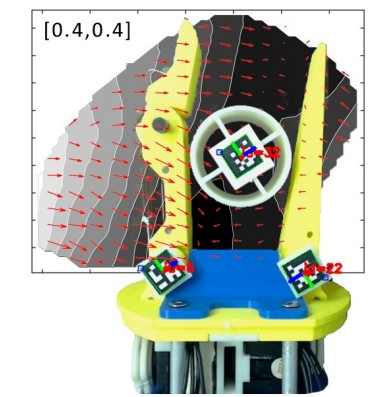
\includegraphics[width=0.3\hsize]{fig/1-introduction/bircher/handsystem.jpg}
	\caption{Robot system \cite{bircher2019}}
	\label{fig::system}
\end{figure}
\begin{figure}[b]
\centering
\begin{minipage}{0.24\hsize}
\centering
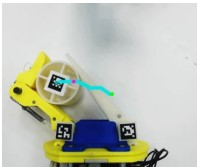
\includegraphics[width=\hsize]{fig/1-introduction/bircher/mani_a.jpg}
\subcaption{}
\end{minipage}
\begin{minipage}{0.24\hsize}
\centering
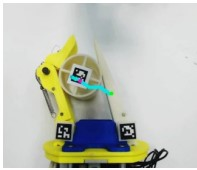
\includegraphics[width=\hsize]{fig/1-introduction/bircher/mani_b.jpg}
\subcaption{}
\end{minipage}	\hfill
\begin{minipage}{0.24\hsize}
\centering
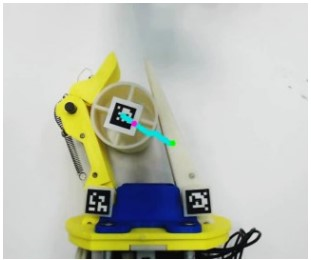
\includegraphics[width=\hsize]{fig/1-introduction/bircher/mani_c.jpg}
\subcaption{}
\end{minipage}	\hfill
\begin{minipage}{0.24\hsize}
\centering
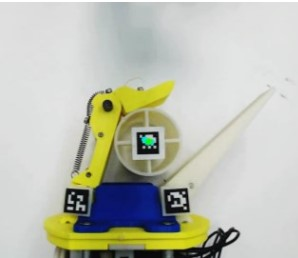
\includegraphics[width=\hsize]{fig/1-introduction/bircher/mani_d.jpg}
\subcaption{}
\end{minipage}	\hfill
\caption{Manipulation results \cite{bircher2019}}
\label{fig::manires}
\end{figure}

\subsubsection{Plannar In-Hand Manipulation Via Motion Cones \cite{chavan-dafle2020}}
この研究では,\figref{fig::maniT}のようにグリッパで対象物を把持し,壁等の外部環境に押し付けたタイミングで把持位置をスライドさせることで持ち替え動作を行っている.ただし,動作計画ではグリッパが固定されており,壁等の環境がプッシャとして対象物を押し出すといった見方をしている.動作計画にあたって,Motion cone (動作円錐)というものを考えている.これは,摩擦の作用を考慮したうえで対象物が1プッシュで到達可能な領域を意味する.動作計画アルゴリズムにはT-RRT*を用いており,ランダムサンプリングしたノードが親ノードのMotion cone内でかつ,効率的な動きである場合,木構造に追加する.Motion cone外であった場合は,Motion cone内に投影した点を用いて同様の判定を行っていた.この手順で枝を伸ばしていき,目標状態となったとき計画を終了している.以上の動作計画のイメージを\figref{fig::rrtimage}に示している.上記の手法に基づき,数多くの実験検証を行い,理論が正確であることが確認されていた.
\begin{figure}
\begin{minipage}{0.49\hsize}
\centering
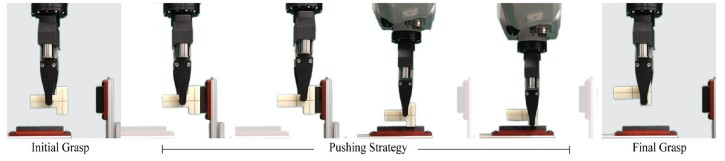
\includegraphics[width=0.9\hsize]{fig/1-introduction/chavan-dafle/manipulation.jpg}
\caption{Manipulating a T-shaped object in a parallel-jaw grasp by pushing it against features in the environment \cite{chavan-dafle2020}}
\label{fig::maniT}
\end{minipage} \hfill
\begin{minipage}{0.49\hsize}
\centering
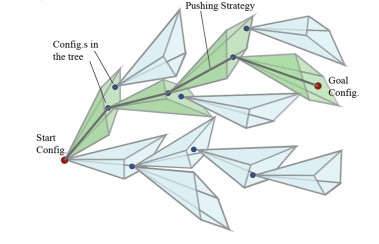
\includegraphics[width=0.8\hsize]{fig/1-introduction/chavan-dafle/rrtimage.jpg}
\caption{The image of motion planner \cite{chavan-dafle2020}}
\label{fig::rrtimage}
\end{minipage}
\end{figure}

\subsubsection{まとめ}
本研究と同じくIn-handマニピュレーションに取り組んだものを紹介した.これらの研究は,マニピュレーション中に対象物に関する力情報や位置情報を必要としており,センシングが不可欠である.この点が本研究との相違点となっている.


\subsection{センサレスなマニピュレーションを行っている研究}
\subsubsection{Sensorless In-Hand Manipulation by An Underactuated Robot Hand \cite{ospina2020}}	\label{sec::ospina}
この研究では,センサレスかつ対象物体の幾何情報なしのIn-handマニピュレーションを提案している.\figref{fig::ohand}のようなハンドを用いており,これは2つのリンクに対して1つのアクチュエータで駆動する劣駆動ハンドとなっている.このハンド先端の円形部分で物体を挟み込み,物体操りを行っている.センサレスなマニピュレーションを実現するため,全ての把持の状態を領域化した,In-hand Manipulability Region (IHMR)というものを定義している.IHMRの範囲内でハンドを動かす限り,把持が成立し続ける.IHMRは物体形状に依存するため,様々な既知物体に対してIHMRを算出し,それらの共通領域を任意物体のIHMRとすることで,幾何情報を必要としないセンサレスin-handマニピュレーションを実現していた.
\begin{figure}[b]
\begin{minipage}{0.49\hsize}
\centering
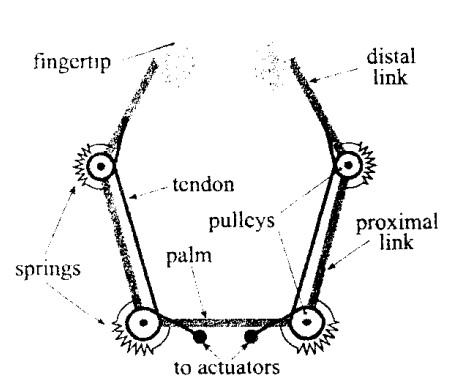
\includegraphics[width=0.9\hsize]{fig/1-introduction/Ospina/handmodel.jpg}
\caption{Two-finger underactuated hand \cite{ospina2020}}
\label{fig::ohand}
\end{minipage} \hfill
\begin{minipage}{0.49\hsize}
\centering
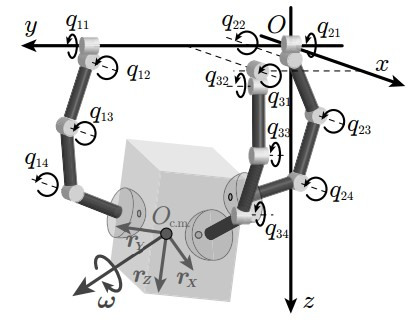
\includegraphics[width=0.9\hsize]{fig/1-introduction/tahara/modeling.jpg}
\caption{Grasping model with three-finger hand \cite{tahara2020}}
\label{fig::model}
\end{minipage}
\end{figure}


\subsubsection{動的安定把持に基づくマニピュレーション \cite{tahara2013}\\多指ロボットハンドによる物体把持のダイナミクスと受動性 \cite{tahara2020}}
この研究では「受動性」の概念を導入することで指が物体と接触している間についてのダイナミクスの特性を解析している.受動性とは簡単に言うと制御における安定性の指標であり,受動性を満たすとき可制御であるとは限らないが,少なくとも内部エネルギーが意図せず増加しない安定状態となっている.\figref{fig::model}のように指先を半球状のモデルで表現し,指先と物体間の接触点位置拘束と転がり速度拘束条件を考慮した運動方程式を立式していた.これに対し,系が受動性を満たすような制御入力を設計することで,安定した把持を実現していた.制御入力はロボットハンドの内界センサ値のみで算出される値であり,センサレスな把持が可能となっていた.

\subsubsection{Sensorless Pose Determination Using  Randomized Action Sequences ~\cite{mannam2019}}
本研究では,\figref{fig::trayrobot}のようにロボットの手先につけたトレーをランダムに何度も傾けることで,物体姿勢のばらつきを定量化したエントロピーを減少させることができることを提案・検証している.ランダムな動作の利点として,物体形状を考える必要がなく,システムが単純であることが挙げられている.実機での検証では,\figref{fig::entropy}のように全体的にみるとエントロピーが減少しており,センサレスで対象物の姿勢をある程度同定できることを示した.
\begin{figure}[b]
\begin{minipage}{0.49\hsize}
\centering
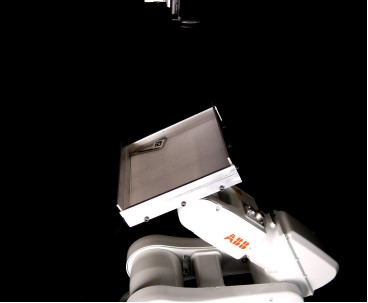
\includegraphics[width=0.9\hsize]{fig/1-introduction/Mannam/trayrobot.jpg}
\caption{An industrial robot with tray \cite{mannam2019}}
\label{fig::trayrobot}
\end{minipage}\hfill
\begin{minipage}{0.49\hsize}
\centering
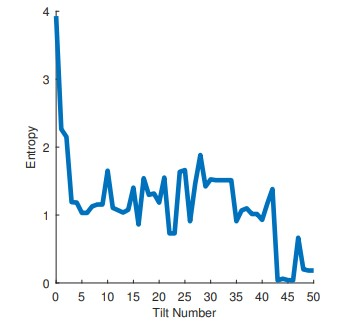
\includegraphics[width=0.9\hsize]{fig/1-introduction/Mannam/entropy.jpg}
\caption{Robot entropy data \cite{mannam2019}}
\label{fig::entropy}
\end{minipage}
\end{figure}

\subsubsection{まとめ}
これらの研究は,センサレスでマニピュレーションを行うという点で本研究と類似している.しかし,以下の観点で本研究の独自性・優位性が主張できる.
\cite{ospina2020}は義手への応用を見込んでおり,把持を維持することに重きを置いているため,把持物体を目標位置・姿勢へ精確に運ぶといったタスクには向かない.\cite{tahara2013}\cite{tahara2020}も同様に把持を安定させることに注力しており,物体の目標位置・姿勢への収束は別の議論が必要である.\cite{mannam2019}はセンサレスかつ物体形状に依存しない点から本研究より汎用性が高いと言える.しかし,整列に非常に長い時間がかかる.本研究のようにパーツフィーダへの応用を前提としている場合,整列時間は生産効率を左右する重要な要素であり,整列時間に優位性があるのは大きなメリットである.


\subsection{パーツフィーダ研究・製品}
%従来のパーツフィーダシステムあったほうがいいかも
\begin{figure}[b]
\begin{minipage}{0.49\hsize}
\centering
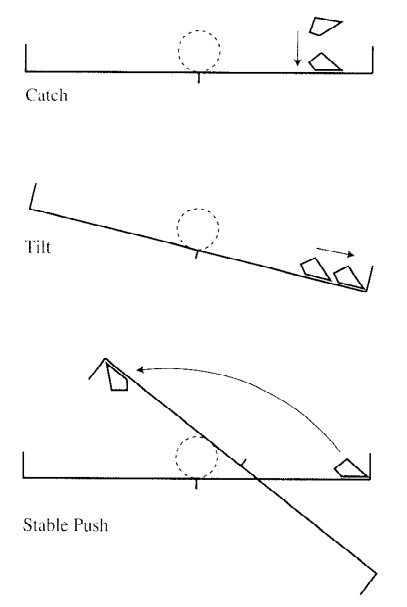
\includegraphics[width=0.9\hsize]{fig/1-introduction/Akella/sensorless_movement.jpg}
\caption{Primitives used for sensorless orienting \cite{akella2000}}
\label{fig::sensmov}
\end{minipage}
\begin{minipage}{0.5\hsize}
\centering
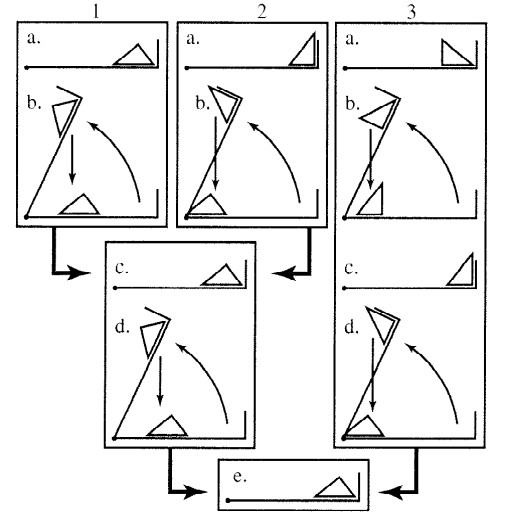
\includegraphics[width=0.9\hsize]{fig/1-introduction/Akella/sensorless_result.jpg}
\caption{Example sensorless feeding plans for a triangle \cite{akella2000}}
\label{fig::sensres}
\end{minipage}
\end{figure}
\subsubsection{Parts Feeding on a Conveyor with a One Joint Robot \cite{akella2000}}
この研究では,\figref{fig::flexfeeder}のように,一つの関節のみを持つロボットとベルトコンベアのみを用いてセンサレスで物体操作を行っている.
\figref{fig::sensmov}の3つの動作のみを用いており,catch動作で対象物の辺をハンドに接触させるところから始まり,物体を目標姿勢へ遷移させることができるような動作組み合わせを計算している.動作例は\figref{fig::sensres}のようになっており,異なる初期状態の対象物に対して同じ目標姿勢へと遷移させていた.
%限界は,凸多角形以外の場合は難しいことが多い,姿勢のみしか整列できない,摩擦なしを仮定,


\begin{figure}[b]
\centering
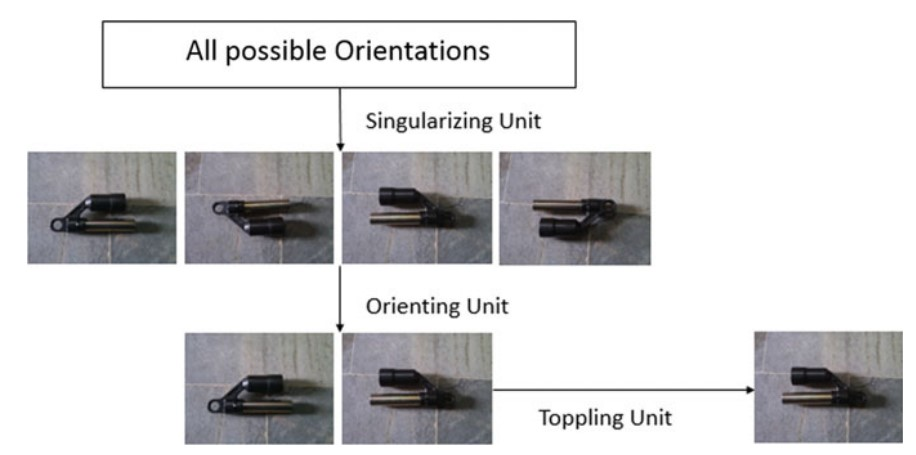
\includegraphics[width=0.6\hsize]{fig/1-introduction/Udhayakumar/threephase.jpg}
\caption{Three phases of orientation \cite{Udhayakumar}}
\label{fig::three}
\end{figure}
\subsubsection{Development of Visionless Flexible Part Feeder for Handling Shock Absorbers \cite{udhayakumar2021}}
この研究では,パーツフィーダの設計・製作から行う安価なシステムを提案している.shock absorberの部品に対象を絞り,次の3手順(\figref{fig::three}),(1) Singularizing Unit,(2) Orienting Unit, (3) Toppling Unit,を順に行い整列していた.(1)は物体を水平方向へ整列させるタスク,(2)は近接センサで上下判定を行い,下向きの場合に上向きに反転させるタスク,(3)は近接センサで左右の向きを検知し,目標姿勢ではない場合は部品を反転させるタスクである.このように,各手順で物体の取りうる姿勢を減らしていくことで,最終的に一つの目標姿勢へと遷移させていた


\subsubsection{まとめ}
\cite{akella2000},\cite{udhayakumar2021}は本研究と同様,物体操作を用いてパーツフィーダを開発している研究である.前者の研究は姿勢のみしか整列できないことが,後者は部品の汎用性がないことがそれぞれ課題としてある.本研究にはこれらを解決できる点で優位性がある.

\subsection{本研究室の従来研究}
本研究室では,「センサレスin-handケージングマニピュレーション」というマニピュレーション手法を提案している.力覚センサを必要とせずハンドの位置制御のみで対象物を拘束できるケージングという考え方を応用することで,対象物を「センサレス」に目標点までマニピュレーションすることができる.
また,ハンド構成に十分な自由度を持たせていることにより,多様な形状の対象物を取り扱えるといった特徴もある.
本手法は,位置・姿勢にばらつきのある対象物を目標の位置・姿勢へと遷移させられるといった特徴から,工場の製造ライン等で乱雑に流れてくる部品を整列させるパーツフィーダへ応用できる.

\subsubsection{センサレスin-handケージングマニピュレーションによる物体の位置・姿勢制御 \cite{komiyama2021}}
以前の研究\cite{asamura2013}では,マニピュレーションにおいて位置の整列のみ行われており,姿勢は考慮されていなかった.それゆえ,円形物体しか取り扱えていなかった.そこで,\cite{komiyama2021}は位置と姿勢の両方を取り扱う手法を提案し,三角形,長方形,L字型等の多様な形状の対象物を取り扱えるようにした.
6自由度ハンドを用いて,上記の対象物に対してマニピュレーションされることを確認していた(\figref{fig::intro::recmani}).
\begin{figure}[b]
\begin{minipage}{0.24\hsize}
\centering
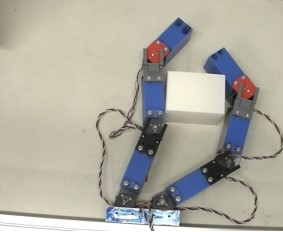
\includegraphics[width=\hsize]{fig/1-introduction/mani1.jpg}
\subcaption{}
\end{minipage}\hfill
\begin{minipage}{0.24\hsize}
\centering
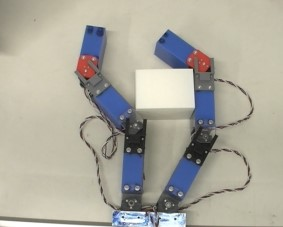
\includegraphics[width=\hsize]{fig/1-introduction/mani2.jpg}
\subcaption{}
\end{minipage}\hfill
\begin{minipage}{0.24\hsize}
\centering
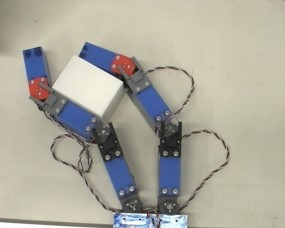
\includegraphics[width=\hsize]{fig/1-introduction/mani3.jpg}
\subcaption{}
\end{minipage}\hfill
\begin{minipage}{0.24\hsize}
\centering
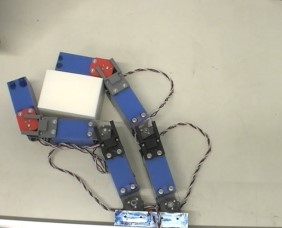
\includegraphics[width=\hsize]{fig/1-introduction/mani4.jpg}
\subcaption{}
\end{minipage}
\caption{Rectangle manipulation \cite{komiyama2021}}
\label{fig::intro::recmani}
\end{figure}

\subsubsection{センサレスin-handケージングマニピュレーションに基づく汎用パーツフィーダの開発 \cite{kamikukita2022}}
この研究では,センサレスin-handケージングマニピュレーションという手法を基に,ベルトコンベアと従来のハンドを用いた汎用パーツフィーダが開発された.ベルトコンベアにより流れてきた対象物に対して,ハンドでキャッチ,マニピュレーション,リリースという一連の動作でパーツフィーダとしての機能を実現していた(\figref{fig::intro::trimani}).また,本手法では180$^\circ$程度の大回転が難しいといった問題点があったが,ベルトコンベアの正転・逆転を利用し,実現していた.
\begin{figure}[b]
\begin{minipage}{0.49\hsize}
\centering
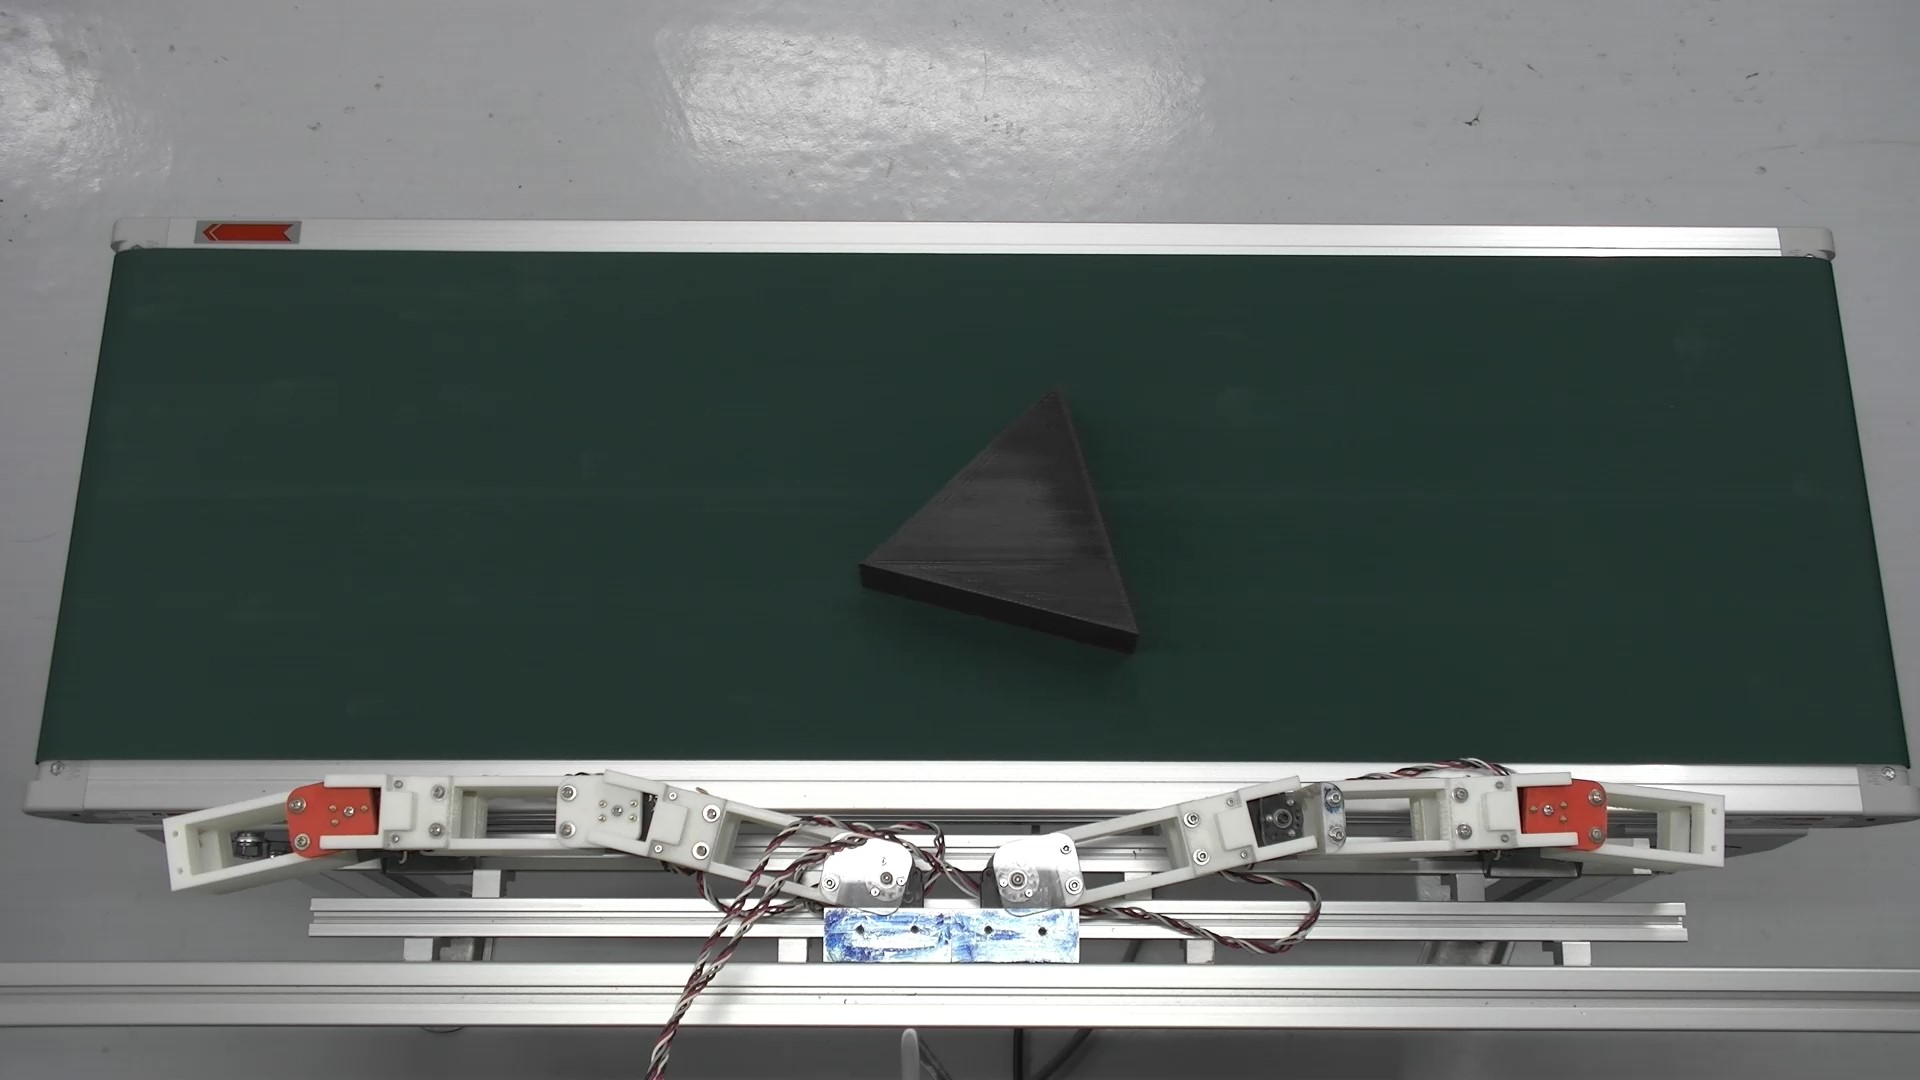
\includegraphics[width=\hsize]{fig/1-introduction/triangle_Moment_2.jpg}
\subcaption{}
\end{minipage}\hfill
\begin{minipage}{0.49\hsize}
\centering
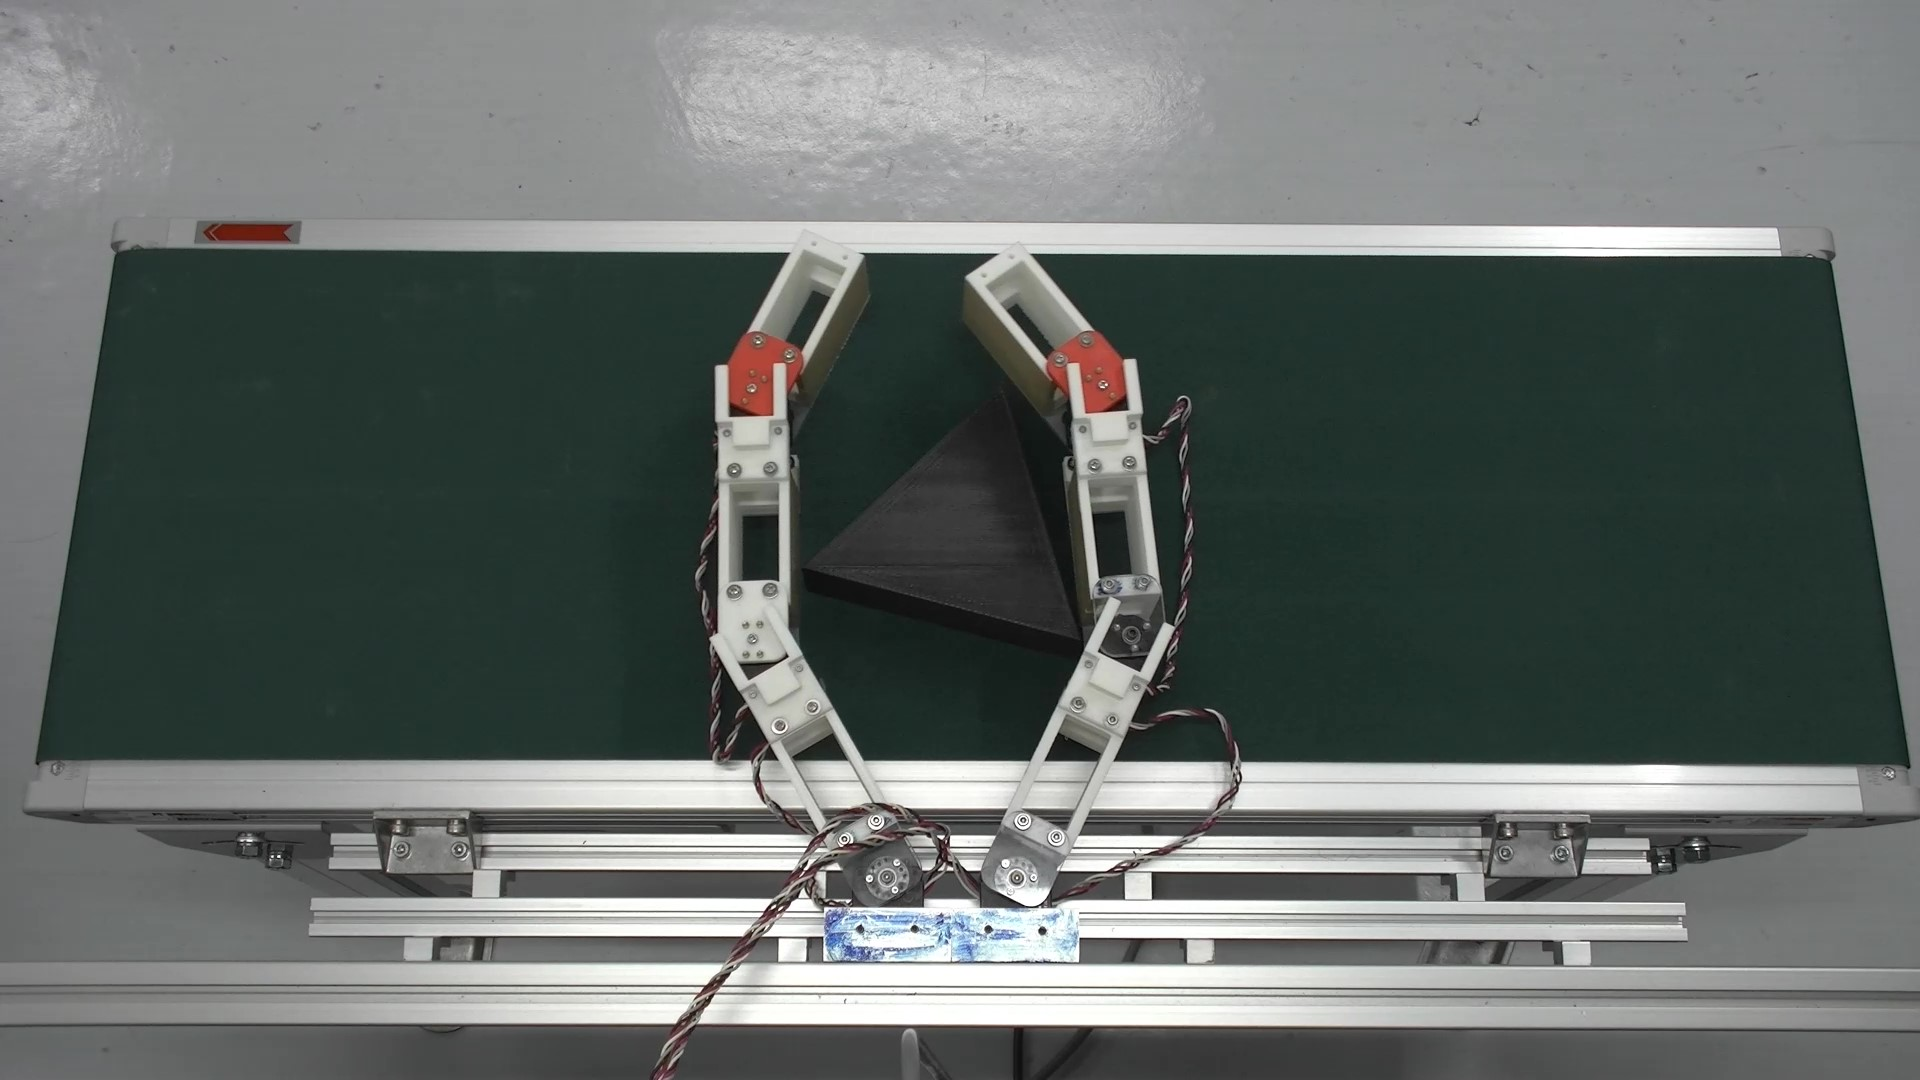
\includegraphics[width=\hsize]{fig/1-introduction/triangle_Moment_3.jpg}
\subcaption{}
\end{minipage}\\
\begin{minipage}{0.49\hsize}
\centering
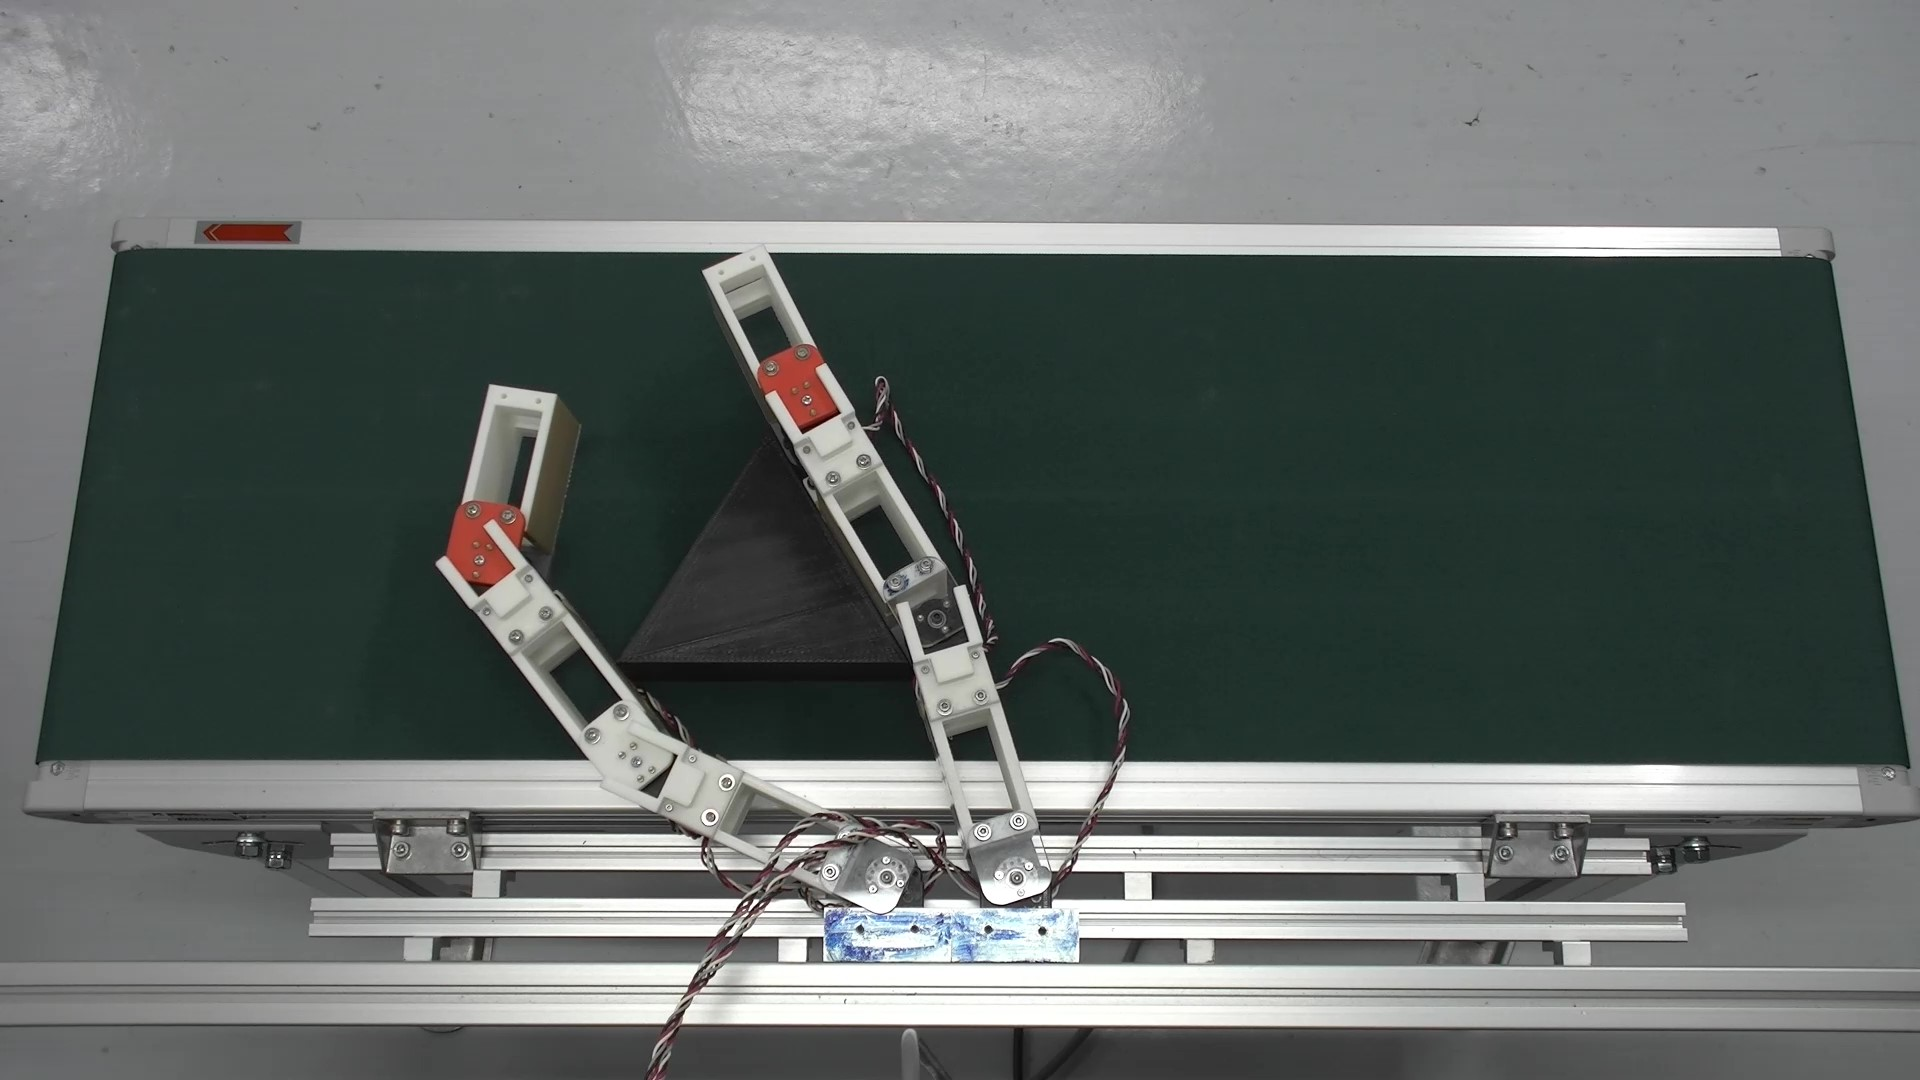
\includegraphics[width=\hsize]{fig/1-introduction/triangle_Moment_5.jpg}
\subcaption{}
\end{minipage}\hfill
\begin{minipage}{0.49\hsize}
\centering
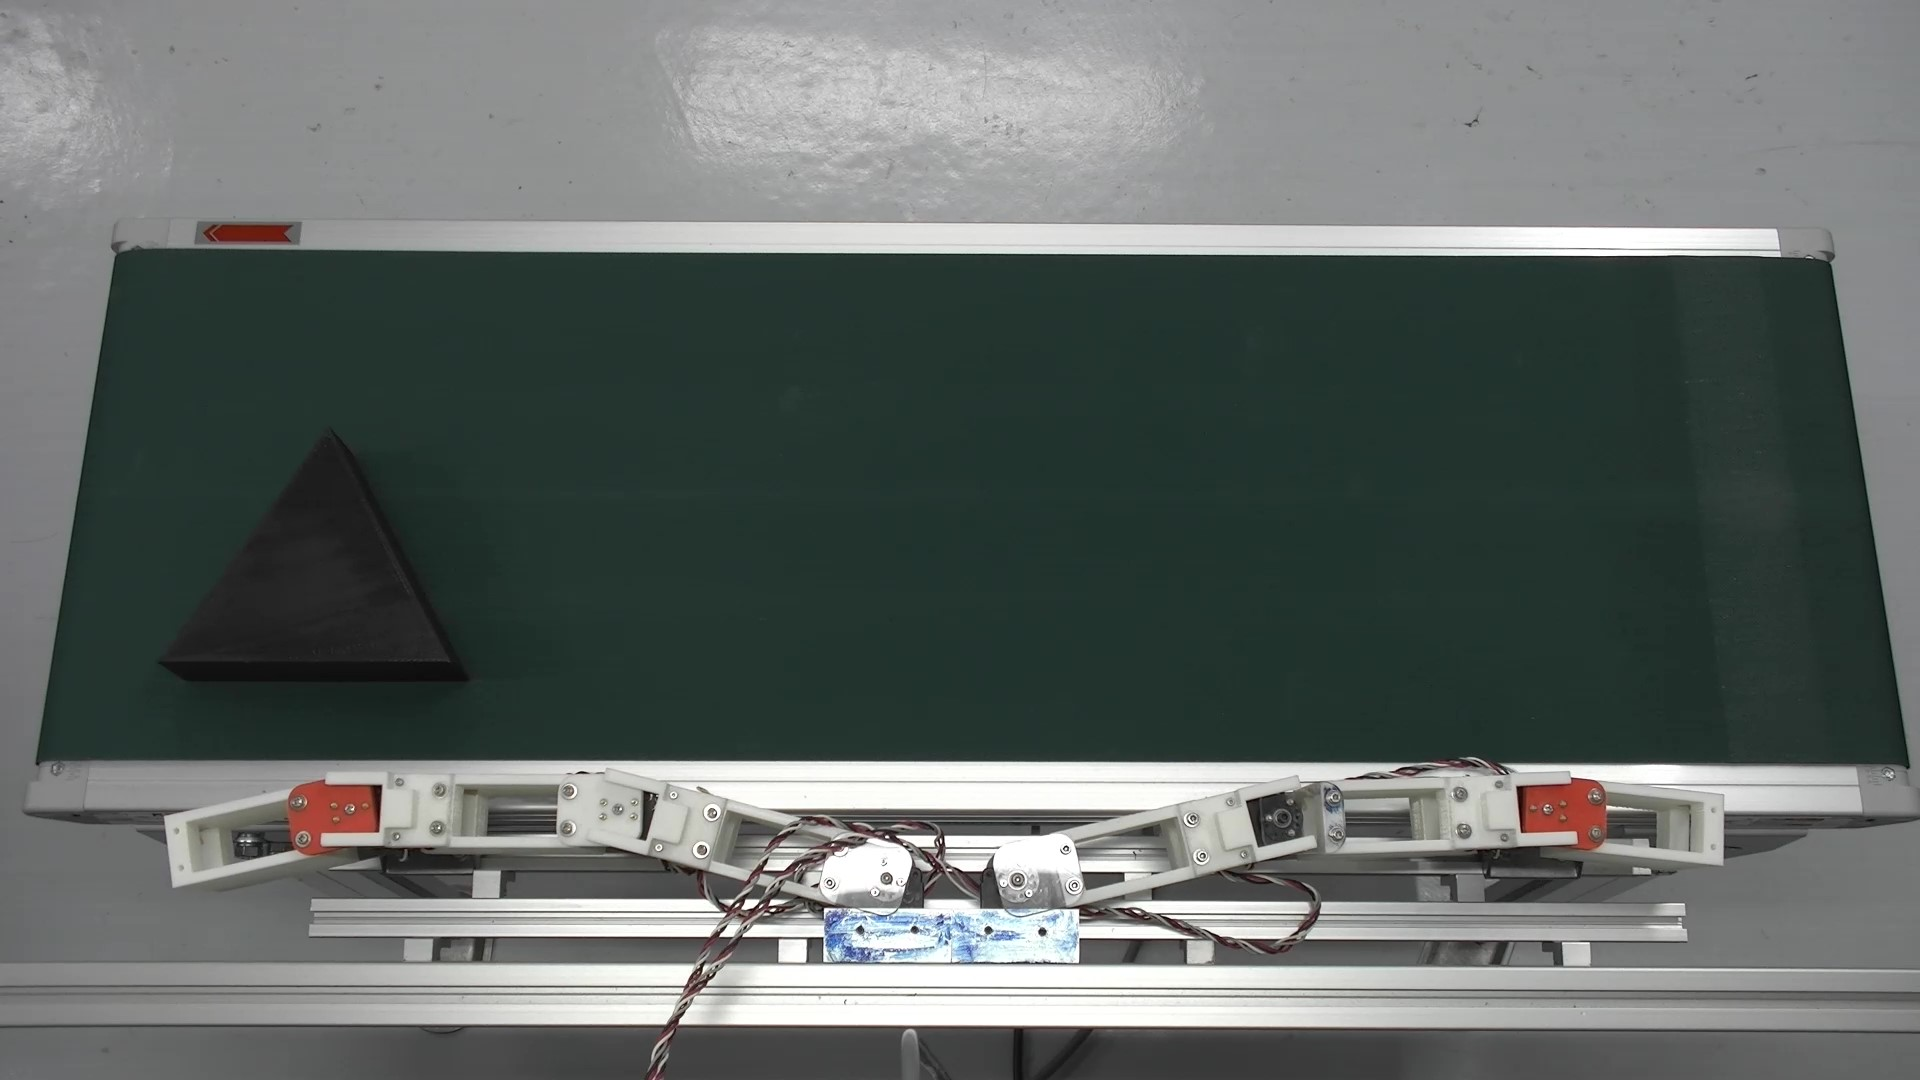
\includegraphics[width=\hsize]{fig/1-introduction/triangle_Moment_7.jpg}
\subcaption{}
\end{minipage}
\caption{Triangle manipulation as part feeder \cite{kamikukita2022}}
\label{fig::intro::trimani}
\end{figure}

\section{研究目的}\label{sec::intro::objective}
\cite{komiyama2021}で,センサレスin-handケージングマニピュレーションにおいて実現したい機能は実装された.しかし,パーツフィーダとしての実用化を目指す上で,以下の課題が存在する.1つ目に対象物がハンドに詰まり,正常にハンドを動かせなくなる「ジャミング」が起きる点,2つ目にハンド動作計画の計算時間が長くかかる点,そして3つ目に対象物の位置決め精度が十分ではないという点である.\par

1つ目に関して,ジャミングは\cite{asamura2013}から存在するセンサレスin-handケージングマニピュレーションの課題である.\cite{komiyama2021}では,ヒューリスティクス的なアプローチで解決を試みた.これにより,ある程度はジャミングを回避できるようになったが,全ての場合に対応できるわけではなく,依然としてジャミングは起こっていた.\cite{kamikukita2022}ではベルトコンベアを用いており,ジャミング時にベルトコンベアを回すことで対象物の状態を変化させ,解消する試みがなされた.この操作を時には複数回繰り返すことで,多くの場合でジャミングを回避できるようになったが,繰り返し操作分,整列時間が長くかかっていた.本手法はパーツフィーダへの応用を見込んでいるので,整列時間の増加は生産効率の低下につながり,望ましくない.

2つ目の計算時間に関しては,一つの動作計画を生成するのに短くとも数時間,長いと数日を要していた.また,3つ目の位置決めは精度は,動作計画時で位置誤差が最大2[cm],姿勢誤差が最大20[deg]生じ得ており,実機の場合はそれ以上の誤差が発生していた.実機精度の向上も必要だが,動作計画の理論計算においてこれほどの誤差が出るのは問題である.本研究においてはこちらを主に取り組む.

2つ目と3つ目の課題はどちらも動作計画に関する課題である.これらの課題は互いに関連しており,計算時間を抑えようとすると位置決め精度が悪くなり,位置決め精度を挙げようとすると計算時間が長くなるという関係にある.

そこで,本論文ではこれらの改善に取り組むべく,以下の2点を目標として掲げる.
\begin{itemize}
\item ジャミングの完全回避
\item 動作計画の総合的な高性能化
\end{itemize}
これにより,センサレスin-handケージングマニピュレーションの有用性が高まり,整列時間,再立ち上げ時間が短く,位置決め精度も高い,パーツフィーダの開発に貢献できると考えている.

\section{本論文の構成}\label{sec::intro::configuration}
本論文の構成を以下に示す.\par
本章では,研究の背景,従来研究を述べ,研究の目的について述べた.\par
2章では,本研究室で提案されてきた平面内センサレスin-handケージングマニピュレーションについて述べる.\par
3章では,従来の動作計画の改良点と新たな動作計画手法について述べる.\par
4章では,提案手法を用いた多角形物体の平面内センサレスin-handケージングマニピュレーションの計画および実機による検証について述べる.\par
5章では,本研究の結論と今後の展望について述べる.


% 白魔術
\expandafter\ifx\csname ifdraft\endcsname\relax
    \end{document}
\fi

% 黒魔術
\expandafter\ifx\csname ifdraft\endcsname\relax
    \documentclass[a4paper,twoside,12pt,papersize, dvipdfmx]{iirthesis}
    \usepackage{amsmath,amssymb,amsthm}
    \usepackage{graphicx}
    \usepackage{subcaption}
    \usepackage{url}
%    \usepackage{otf}
    \usepackage{minitoc}
    \usepackage{bm}
    \usepackage{amsmath,amssymb}
    \begin{document}

    \newcommand{\figref}[1]{\figurename\ref{#1}}
    \newcommand{\tabref}[1]{\tablename\ref{#1}}
    \renewcommand{\eqref}[1]{式~(\ref{#1})}
    \newcommand{\chapref}[1]{\ref{#1}章}
    \newcommand{\secref}[1]{\ref{#1}節}
    \newcommand{\ssecref}[1]{\ref{#1}項}
    \newcommand{\appref}[1]{付録\ref{#1}}
\fi


\chapter{平面内センサレスin-handケージングマニピュレーション}\label{chap::sicm}
\minitoc

\section{概要}
\cite{asamura2013}で,「センサレスin-handケージングマニピュレーション」という新たなマニピュレーション手法が提案された.これは,ロボットハンドの位置制御のみで対象物を拘束できる「ケージング」\cite{rimon1999}を基にしたマニピュレーション手法である.ケージングは,ロボットハンドと対象物の間の力のつり合いによって対象物を拘束する把持とは異なり,対象物の形状情報を基に幾何学的に囲い込むことで拘束する.そのため,力情報を必要としない.また,「囲い」による拘束であるため,対象物の詳細な位置情報も必要としない.一般的なIn-handマニピュレーション手法では,対象物の位置情報や力情報を必要とするが,本手法ではケージングを利用することにより,センサレスなマニピュレーションが可能となっている.\par
本手法の特徴として,上述のセンサを必要としないことに加えて,外乱に強いといった点も挙げられる.センサレスin-handケージングマニピュレーションでは,マニピュレーション中は常に対象物のケージングが成立している.そのため,マニピュレーション中に対象物に外乱が加わり位置・姿勢に変化が生じても,最後までマニピュレーションを行うことができる.\par
本手法は,センサを用いていないため,動作計画において対象物の正確な位置・姿勢情報を扱うことはできない.しかし,対象物の形状情報は既知なので,ケージングが成立している任意のハンド姿勢による囲い内において,対象物が存在できる位置・姿勢群を算出できる.そこで,ケージングに関する条件を満たしながら,囲いの形状を変化させていく過程で,対象物が存在できる位置・姿勢群の数を十分に減らし,かつ目標位置・姿勢付近へと十分に近づけることで,センサレスに対象物を目標位置・姿勢へと位置決めすることができる.\par
以下の節では,より具体的な説明を行っていく.\secref{sec::sicm::partsfeeder}では,センサレスin-handケージングマニピュレーションを行うためのシステムの説明を行う.また,新たなハンド構成の提案についても記述する.\secref{sec::sicm::cspace}では,対象物の位置・姿勢群の扱い方について,\secref{sec::sicm::caging}では,センサレスin-handケージングマニピュレーションを可能とするためのケージングに関する条件について,\secref{sec::sicm::planning}では,動作計画に使用しているアルゴリズムについて述べる.
%ケージングを用いることでセンサを必要としないこと
%オフラインで事前生成要素も書ければ書きたい

\section{汎用パーツフィーダ}\label{sec::sicm::partsfeeder}
センサレスin-handケージングマニピュレーションの位置・姿勢にばらつきのある対象物を特定の位置・姿勢に整列できるという機能を活かして,本手法はパーツフィーダへ応用することを見込んでいる.本研究では,ベルトコンベアと1対のロボットハンドを用いて\figref{fig::sicm::overview}のように構成している.ロボットハンドは,3つのリンク,3つの関節からなる3自由度ハンドとなっている.ここで,\figref{fig::sicm::overview}のように1対のロボットハンドを並列に並べたハンド構成を並列型ハンドと呼ぶこととする.
\subsection{一連の動作の流れ\cite{kamikukita2022}}\label{subsec::sicm::flow}
パーツフィーダの動作の流れについて説明する(\figref{fig::sicm::overview}).まず,ハンドを開いた状態で,ベルトコンベアにより対象物を一定時間移動させ,停止する.その後,ハンドを閉じて物体を囲み,対象物のケージング状態を作った後にマニピュレーションを行う.整列が終了すると,ハンドを開いて物体を開放し,ベルトコンベアを一定時間動かして,対象物を流出させる.\par
%本来のパーツフィーダでは,物体の分離と整列が必要となるが,本研究で扱うパーツフィーダは,物体の分離は行わず,ベルトコンベア上に十分な間隔で物体があることを前提として物体の整列動作を行う.

\begin{figure}[b]
\centering
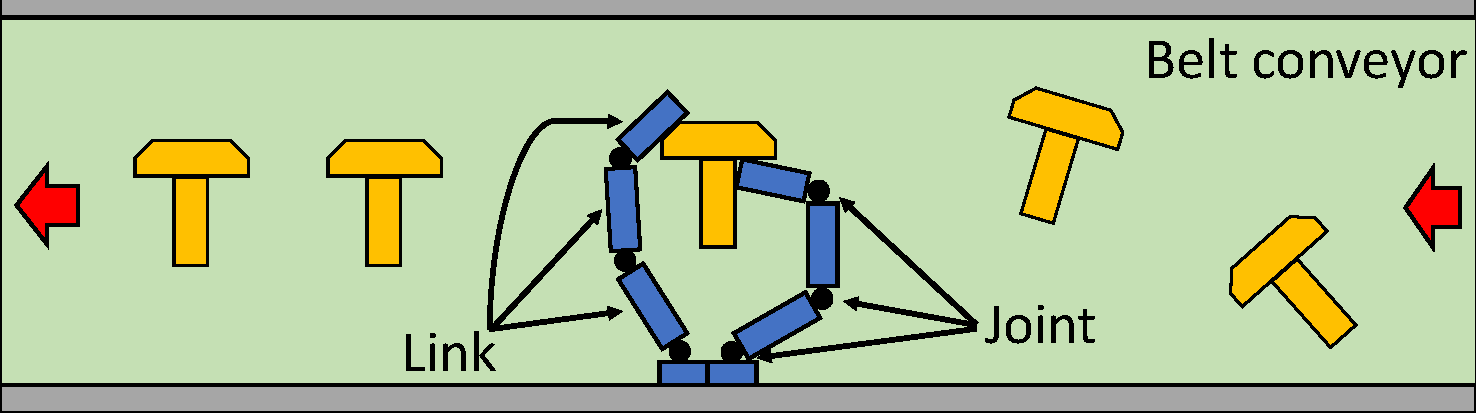
\includegraphics[width=0.9\hsize]{fig/2-sensorless-icm/systemoverview.pdf}
\caption{System overview} \label{fig::sicm::overview}
\end{figure}

\subsection{対向型ハンド}\label{subsec::sicm::oppositehand}
\secref{sec::intro::objective}で述べた通り,並列型ハンドでは対象物がハンド根元付近に詰まり,ハンドが正常に動けなくなるジャミング(\figref{fig::sicm::jam})が発生していた.また,並列型ハンドの構造上,ハンド根元関節付近に対象物が存在する場合,マニピュレーションできないといった問題点も存在した.\par
そこで,\figref{fig::sicm::opposite-hand}のようなハンド構成,対向型ハンドを提案する.
前者の問題に関して考える.並列型ハンドでは,根元付近に対象物がある場合,根元リンクのみで対象物を扱わなければならない.根元リンクは自由度が低く,発揮できる力の方向も限られている.そのため,一度ジャミングが起こると基本的にはハンドを開く方向に動かすことでしか回避できないが,通常,ハンドは目標位置・姿勢に向けて狭まっていく.これがジャミング回避が困難な理由である.一方,対向型ハンドでは手先のリンクが使える.手先リンクは自由度が高く,様々な方向へ力を発揮できる.そのため,ジャミングが起こりそうになると,それを回避するような状態が取られる.以上より,ジャミング解消が期待できる.
後者の問題に関して,対向型ハンドでは,縦方向にはどの場所に対象物が存在してもマニピュレーションすることができる.しかし,横方向は並列型ハンドほど広く扱えない.しかし,横方向の移動はベルトコンベアで賄えるので,大きな問題ではないと考えている.
\begin{figure}[b]
	\centering
	\begin{minipage}{0.33\hsize}
	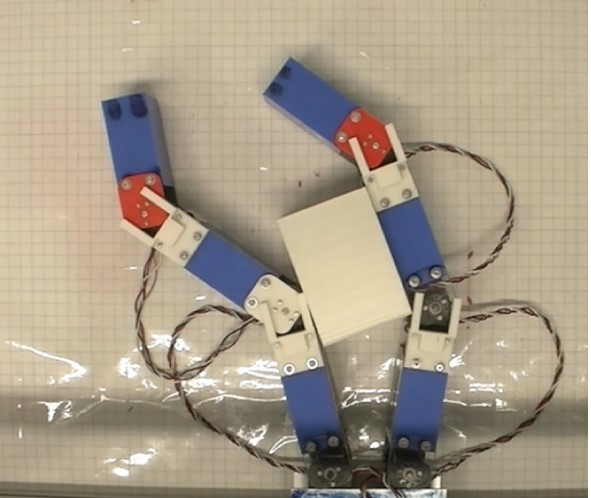
\includegraphics[width=0.9\hsize]{fig/2-sensorless-icm/jam1.jpg}
	\subcaption{Before jam}\label{fig::sicm::beforejam}
	\end{minipage}\hfill
	\begin{minipage}{0.33\hsize}
	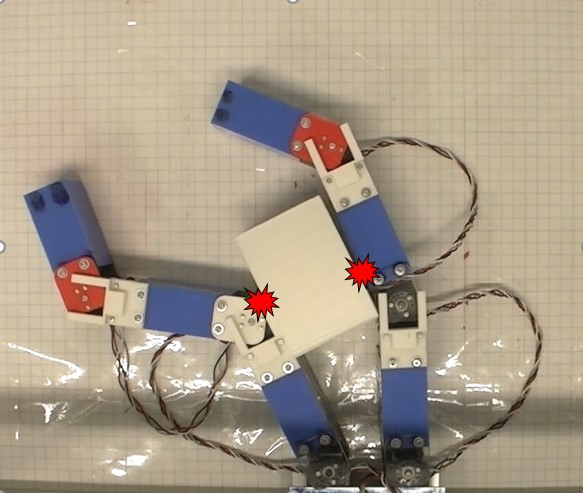
\includegraphics[width=0.9\hsize]{fig/2-sensorless-icm/jam2.jpg}
	\subcaption{Just jammed}\label{fig::sicm::justjam}
	\end{minipage}\hfill
	\begin{minipage}{0.33\hsize}
	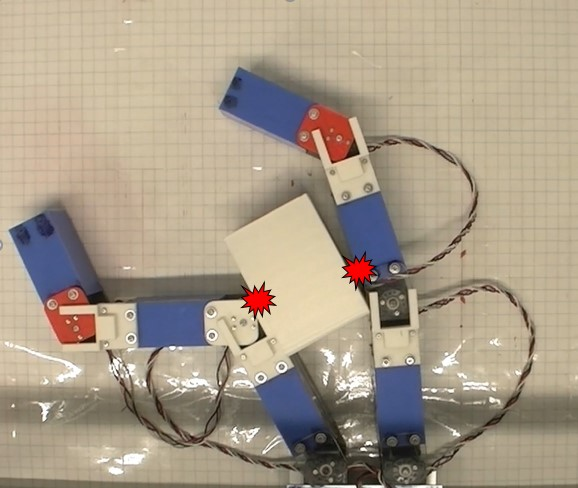
\includegraphics[width=0.9\hsize]{fig/2-sensorless-icm/jam3.jpg}
	\subcaption{Still jammed}\label{fig::sicm::stilljam}
	\end{minipage}
	\caption{Manipulation by parallel-type hand (Jamming occuring)}
	\label{fig::sicm::jam}
	

	\centering
	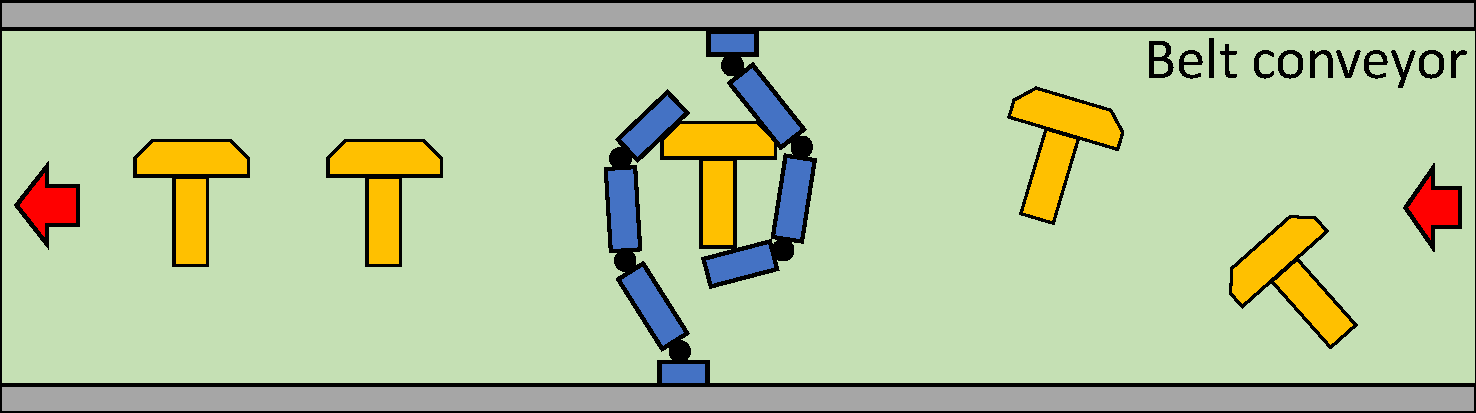
\includegraphics[width=0.9\hsize]{fig/2-sensorless-icm/opposite-type.pdf}
	\caption{Opposite-type hand} \label{fig::sicm::opposite-hand}
\end{figure}

\section{対象物のコンフィギュレーション空間\cite{komiyama2021}}\label{sec::sicm::cspace}
本節では,ハンド動作計画の際に使用する,対象物のコンフィギュレーション空間について説明する.我々は対象物の状態を,位置$(x, y)$と姿勢(傾き)$\phi$の3変数によって表している.この3変数で構成される3次元空間が対象物のコンフィギュレーション空間である.空間内の任意の座標は,対象物の任意の位置・姿勢を表しており,それぞれ1:1に対応している.\par

このコンフィギュレーション空間の中から,対象物が存在できる領域を対象物のコンフィギュレーション自由空間と呼び,$C_{\mathrm{free}}$と表す.具体的な$C_{\mathrm{free}}$の導出は以下の通りである.まず,任意の座標$(x, y, \phi)$に対して,対象物の代表点を$(x, y)$に合わせ,$\phi$だけ傾ける.このとき\figref{fig::sicm::cfree}(a)のようにハンドにも壁にも干渉しない場合,任意の座標$(x, y, \phi)$は$C_{\mathrm{free}}$を構成する点として認められ,\figref{fig::sicm::cfree}(b)のように干渉した場合は,$C_{\mathrm{free}}$を構成する点としては認めない.この判定を空間全体に対して行ったときの前者の集合が$C_{\mathrm{free}}$となる.
\begin{figure}[b]
\begin{minipage}{0.5\hsize}
\centering
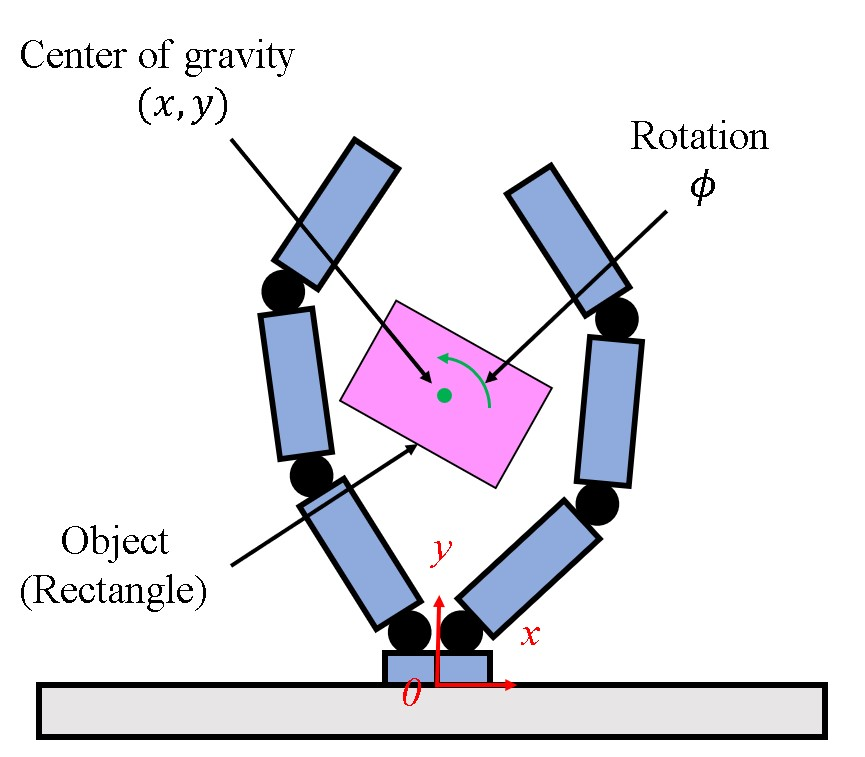
\includegraphics[width=0.9\hsize]{fig/2-sensorless-icm/define_cfree.jpg}
\end{minipage}
\begin{minipage}{0.5\hsize}
\centering
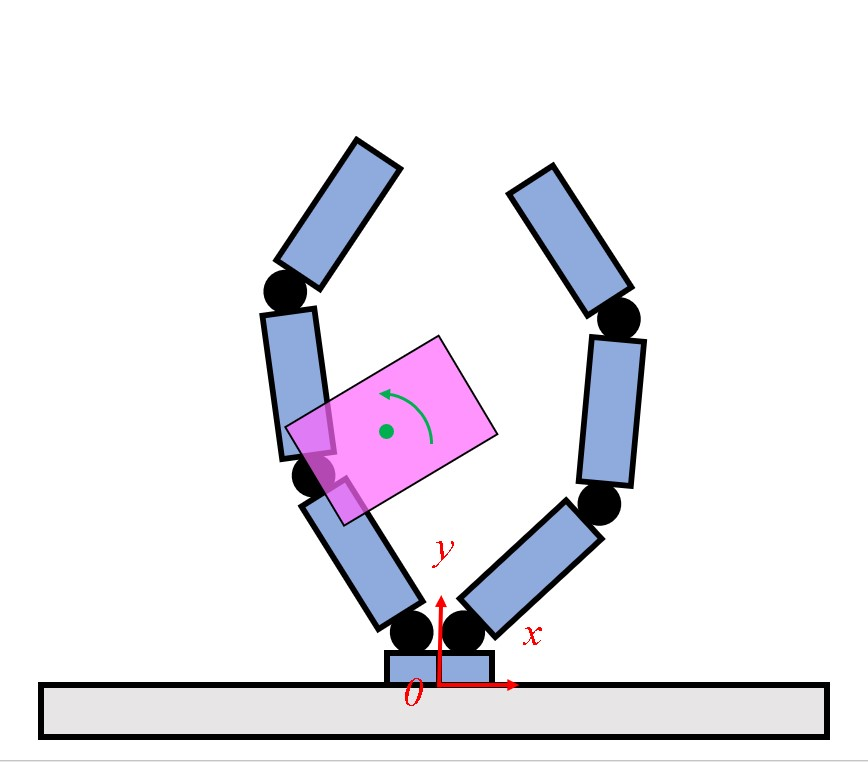
\includegraphics[width=0.9\hsize]{fig/2-sensorless-icm/define_notcfree.jpg}
\end{minipage}
\caption{Definition of $C_{\mathrm{free}}$}
\label{fig::sicm::cfree}
\end{figure}

実装にあたり,対象物のコンフィギュレーション空間を\figref{fig::sicm::discretize}のように格子状に分割し,離散的に取り扱っている.本来,コンフィギュレーション空間は連続した空間である.そのため,格子点の幅を狭めれば狭めるほど実際の表現に近くなる.一方で,格子点幅を狭めすぎると格子点数が増え,その分計算負荷が大きくなる.したがって,マニピュレーションの動作計画に支障のない範囲で格子点幅を確保しつつ,計算負荷も抑えられるようなバランスの良いパラメータ設定が重要となる.\par

一例として,6自由度並列型ハンドで長方形物体をケージングした際の対象物コンフィギュレーション$C_{\mathrm{free}}$を\figref{fig::sicm::cfreeexam}に示す.緑色領域が$C_{\mathrm{free}}$であり,この$C_{\mathrm{free}}$を評価することで,現在のハンド姿勢がセンサレスin-handケージングマニピュレーションするにあたって,妥当な姿勢か否かを判定する.この判定については,次節で説明する.

\begin{figure}[hb]
\centering
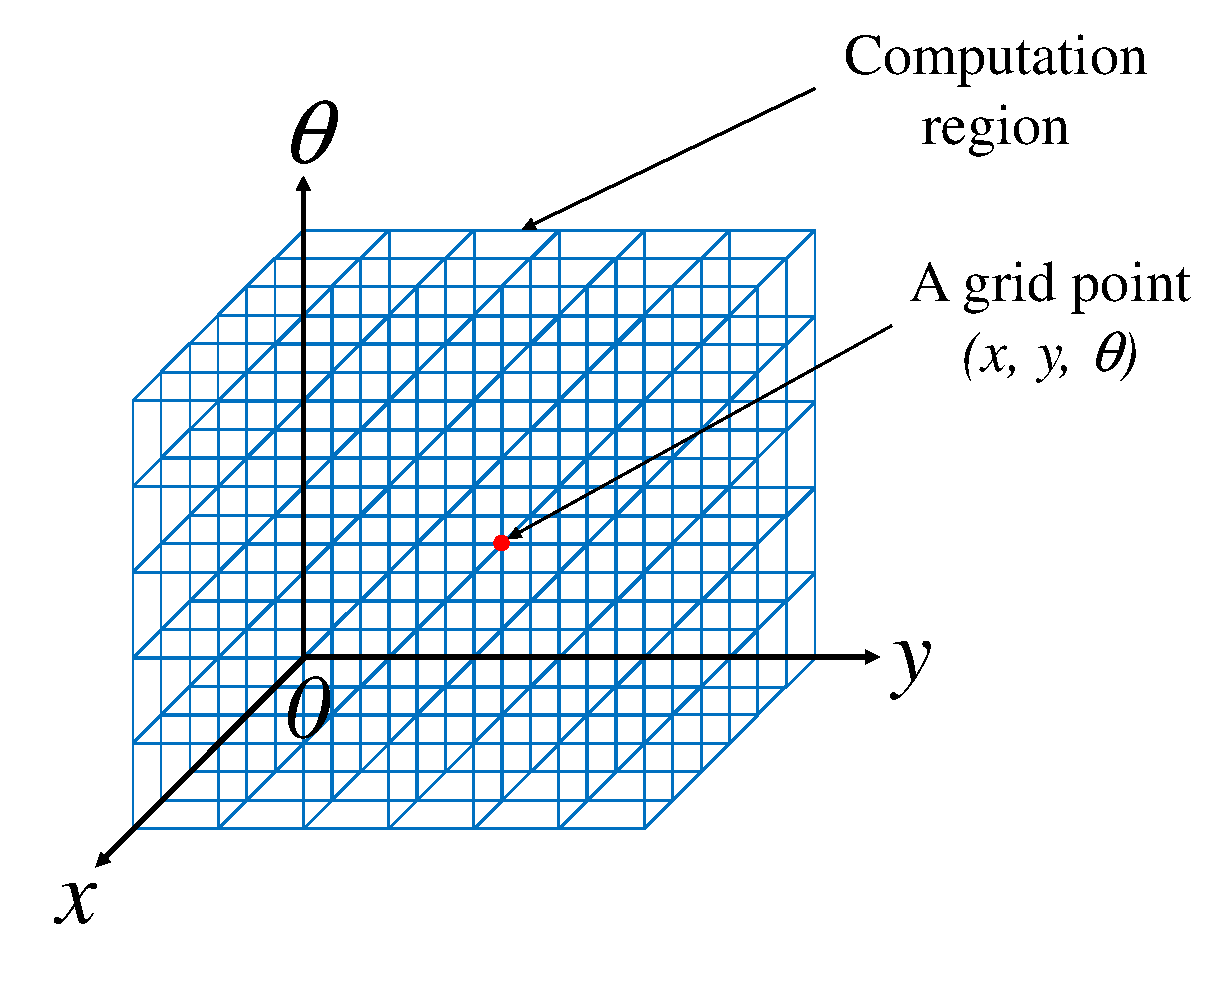
\includegraphics[width=0.6\hsize]{fig/2-sensorless-icm/DiscretizeSpace.pdf}
\caption{Discretization of the 3D computation region \cite{komiyama2021}}
\label{fig::sicm::discretize}

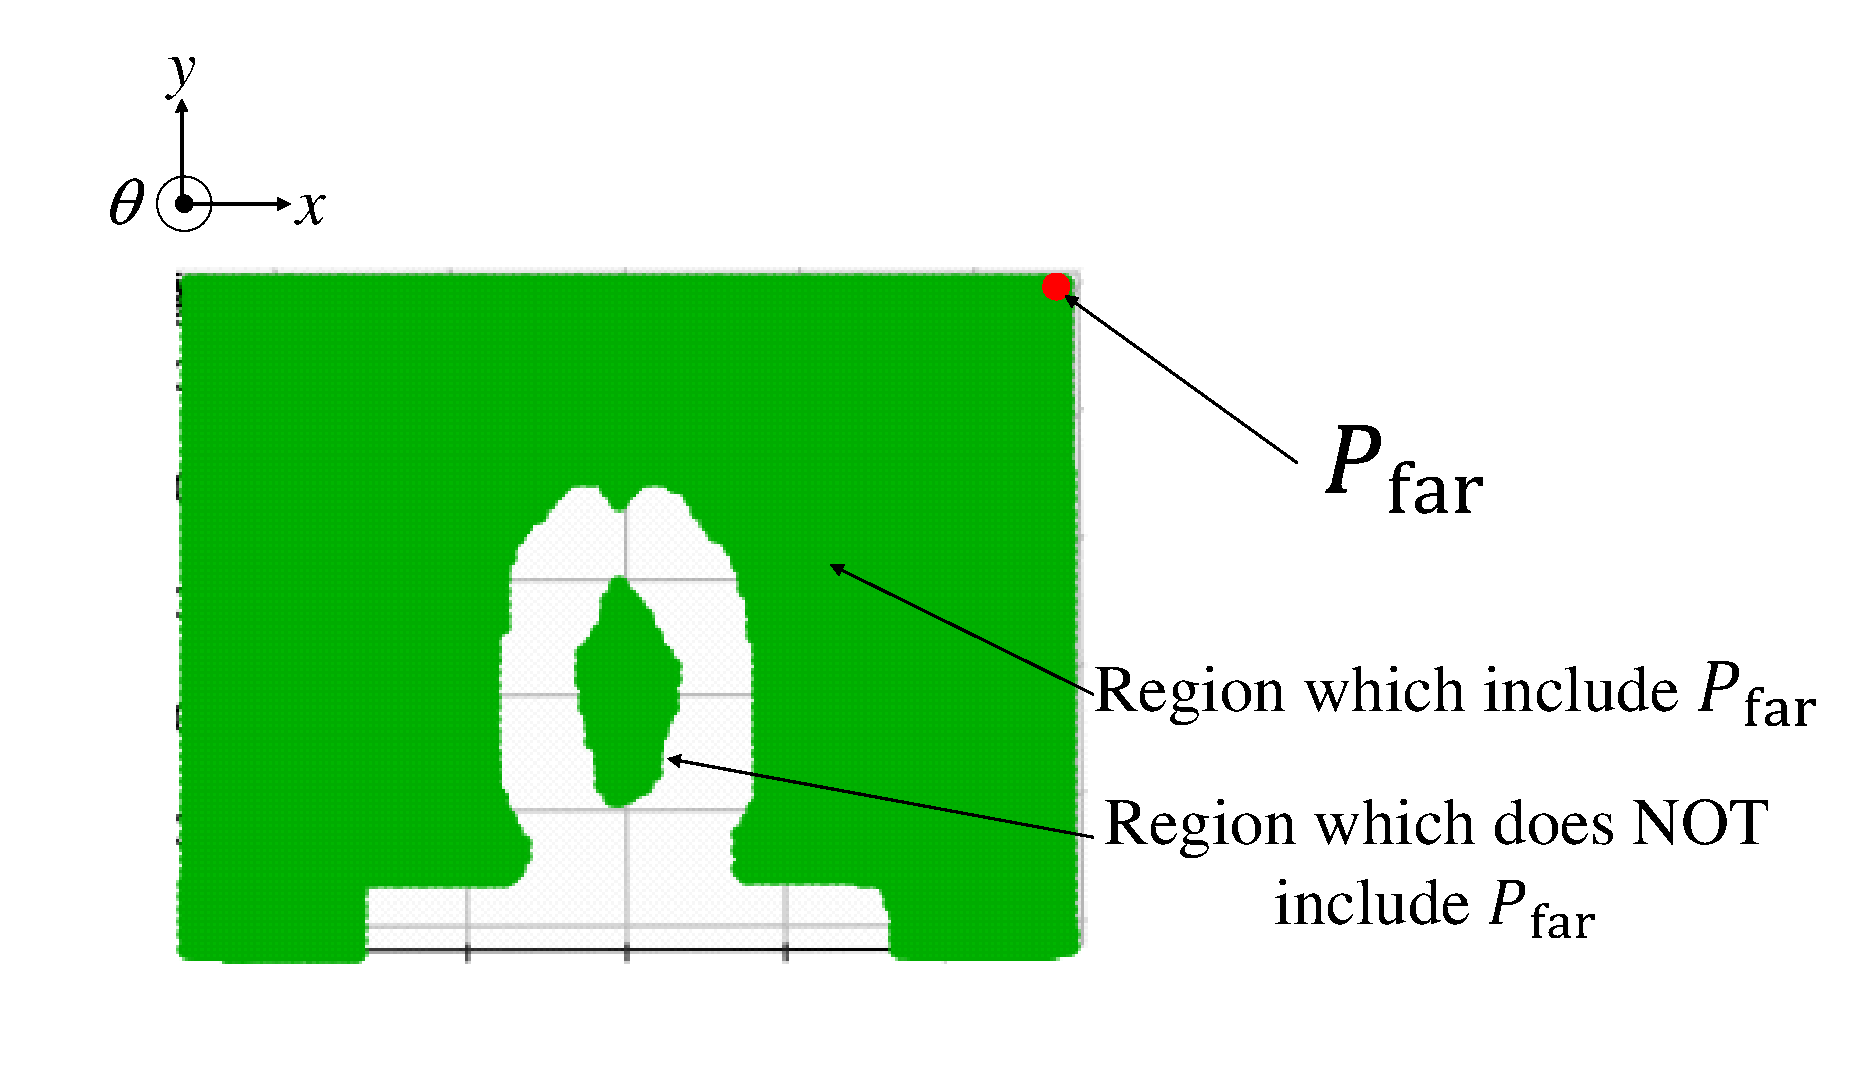
\includegraphics[width=0.7\hsize]{fig/2-sensorless-icm/cfree.pdf}
\caption{The configuration free space ($\mathcal{C}_{\mathrm{free}}$) of the object \cite{komiyama2021}}
\label{fig::sicm::cfreeexam}
\end{figure}


\section{ケージング成立条件とケージングマニピュレーション可能条件\cite{komiyama2021}}\label{sec::sicm::caging}
\subsection*{ケージング成立条件}
ケージング条件の説明にあたり,以下のように記号を定義する.
\begin{itemize}
\item $\mathcal{C}$: 物体のコンフィギュレーション空間
\item $\mathcal{A}_{\mathrm{obj}}$: 実空間での物体の領域
\item $\mathcal{A}_{\mathrm{finger}}$: 実空間でのロボットハンドの指部分の領域
\item $\mathcal{A}_{\mathrm{palm}}$: 実空間でのロボットハンドのパームの領域
\item $\bm{q}_{\mathrm{obj}}$: 物体のコンフィギュレーション
\item $\bm{q}_{\mathrm{finger}}$: ハンドの指部分のコンフィギュレーション
% \item $\bm{q}_{\mathrm{goal}}$: ハンドの指部分の目標コンフィギュレーション
\end{itemize}

まず,\secref{sec::sicm::cspace}で述べた,対象物がハンドやロボットと干渉せず存在できる位置・姿勢群であるコンフィギュレーション自由空間$\mathcal{C}_{\mathrm{free}}$は,上記の記号を用いて次のように表される.
\begin{gather}
\mathcal{C}_{\mathrm{free}} :=
\{\bm{q}_{\mathrm{obj}} \in \mathcal{C} | \mathcal{A}_{\mathrm{obj}}(\bm{q}_{\mathrm{obj}})
\cap \mathcal{A}_{\mathrm{finger}}(\bm{q}_{\mathrm{finger}}) \neq \varnothing\}
\label{eq::cfree}
\end{gather}

対象物のケージングが成立している場合,\figref{fig::sicm::cfreeexam}のように$\mathcal{C}_{\mathrm{free}}$は少なくとも2つ以上の連結した領域に分割される.これらの領域は2つのグループに分けられる.1つは,ハンドによって囲われ,ハンド内部で独立している領域.もう1つは,ハンド外部と接続された領域である.前者は対象物がハンド内部から出ることができないことを意味するためICS (Inescapable Configuration Space)と,後者は対象物がハンド外部へ自由に逃げられることを意味するためECS (Escapable Configuration Space)と呼ぶ(\figref{fig::sicm::cfreeics}).これらに属するコンフィギュレーション自由空間をそれぞれ$\mathcal{C}_{\mathrm{free\_ICS}}$,$\mathcal{C}_{\mathrm{free\_ECS}}$と定義する.$\mathcal{C}_{\mathrm{free\_ICS}}$,$\mathcal{C}_{\mathrm{free\_ECS}}$は,以下のような式で表される.


\begin{gather}
\mathcal{C}_{\mathrm{free\_ECS}} := 
\bigcup_{\bm{q}_{\mathrm{obj}}\in P_{\mathrm{far}}}
\mathcal{C}_{\mathrm{free\_max}}(\bm{q}_{\mathrm{obj}}) \\
\mathcal{C}_{\mathrm{free\_ICS}} := \mathcal{C}_{\mathrm{free}} 
\setminus \mathcal{C}_{\mathrm{free\_ECS}}
\end{gather}

ここで,$P_{\mathrm{far}}$は,ロボットハンドによって囲われる可能性のない無限遠点を指す.$\mathcal{C}_{\mathrm{free}}$の内,$P_{\mathrm{far}} (\subset \mathcal{C})$を含む領域を$\mathcal{C}_{\mathrm{free\_ECS}}$と,$P_{\mathrm{far}} (\subset \mathcal{C})$を含まない領域を$\mathcal{C}_{\mathrm{free\_ICS}}$と判定する.\par

$\mathcal{C}_{\mathrm{free\_ICS}}$は複数の領域から構成される場合がある.言い換えると,対象物がハンド内部で取りうる位置・姿勢群は数パターンある場合がある.この内,実際に対象物が存在している領域はいずれか一つであり,この領域を$\mathcal{C}_{\mathrm{free\_obj}}$と定義する.式では以下のようにあらわせる.
\begin{gather}
\mathcal{C}_{\mathrm{free\_obj}} \subseteq \mathcal{C}_{\mathrm{free\_ICS}}
\end{gather}

ここで,センサレスに$\mathcal{C}_{\mathrm{free\_obj}}$領域を特定するため,$\mathcal{C}_{\mathrm{free\_obj}}$の連続性を考える.つまり,対象物が実際に取りうる位置・姿勢群$\mathcal{C}_{\mathrm{free\_obj}}$は,直前$(t-\Delta t)$のハンド姿勢のものと現在$(t)$のハンド姿勢のものでは連続性の観点からオーバーラップしていると考える(\eqref{eq::sicm::continuous}).
\begin{gather}\label{eq::sicm::continuous}
\mathcal{C}_{\mathrm{free\_obj}}(t-\Delta t) \cap 
\mathcal{C}_{\mathrm{free\_obj}}(t) \neq \varnothing
\end{gather}
これを基に,$\mathcal{C}_{\mathrm{free\_obj}}(t-\Delta t)$とオーバーラップする$\mathcal{C}_{\mathrm{free\_ICS}}(t)$を取り出すことで,$\mathcal{C}_{\mathrm{free\_obj}}(t)$が抽出される.$\mathcal{C}_{\mathrm{free\_obj}}(t=0)$は既知であるため,全ての時刻$t$において帰納的に特定できる.

ケージング成立条件は,対象物が実際に取りうる位置・姿勢群がハンドによって完全に囲われ,外部に逃げられないことを保証するもので,以下の式で表せる.
\begin{gather}
\mathcal{C}_{\mathrm{free\_obj}} \neq \varnothing
\end{gather}

\begin{figure}[hb]
\centering
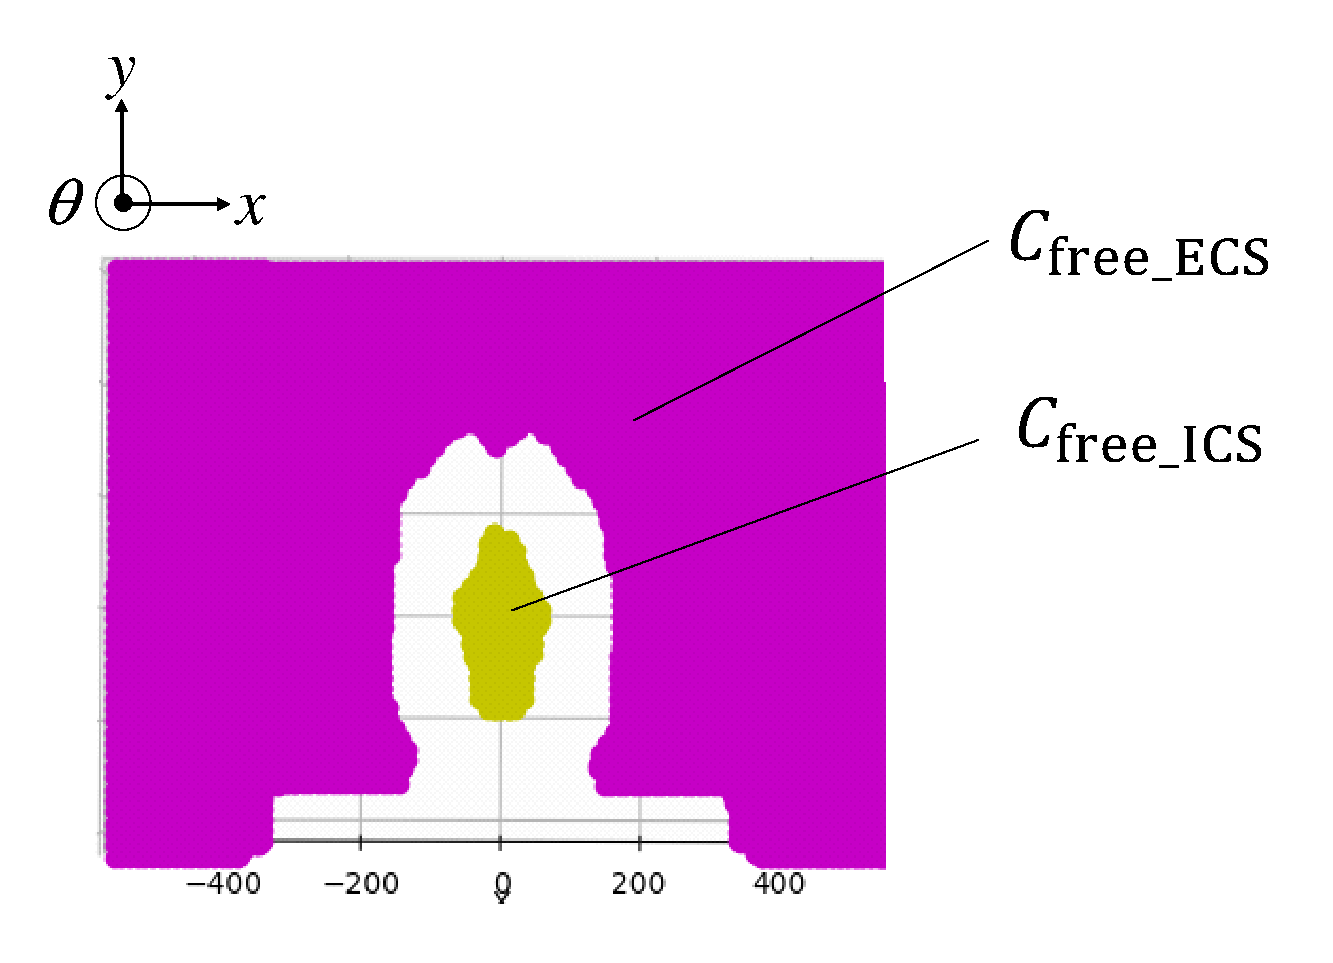
\includegraphics[width=0.6\hsize]{fig/2-sensorless-icm/cfree_ics.pdf}
\caption{$\mathcal{C}_{\mathrm{free}}$ can be classified into $\mathcal{C}_{\mathrm{free\_ICS}}$ or $\mathcal{C}_{\mathrm{free\_ECS}}$ \cite{komiyama2021}}\label{fig::sicm::cfreeics}
\end{figure}

\clearpage
\subsection*{ケージングマニピュレーション可能条件}
ケージングマニピュレーション可能条件とは,センサレスな本手法において対象物の状態を確実に追跡するための条件である.先述の方法で,$\mathcal{C}_{\mathrm{free\_obj}}(t)$の抽出を行うと,複数の領域が得られる場合がある.この場合,対象物が$\mathcal{C}_{\mathrm{free\_obj}}(t-\Delta t)$から実際にどの領域へ遷移したか特定できない.この状態が続くと,対象物を最終的な目標位置・姿勢へマニピュレーションできなくなる.このような事態を防ぐため,以下の条件をケージングマニピュレーション可能条件として定めている.
\begin{itemize}
\item $\mathcal{C}_{\mathrm{free\_obj}}$が1つの領域のみにより構成される
\end{itemize}

\figref{fig::scim::divided1},\figref{fig::sicm::divided2}は,ハンド姿勢のわずかな変化で$\mathcal{C}_{\mathrm{free\_obj}}$が二つの領域に分裂する場合の例を示している.\par
$\mathcal{C}_{\mathrm{free\_obj}}$が一度分裂しても,後のハンド姿勢の変化によって,分裂した領域が再び一つになる場合がある.このような場合,それ以後のマニピュレーションは問題なく進むものと考えられるが,動作計画の際に,分裂した$\mathcal{C}_{\mathrm{free\_obj}}$の領域全てを追跡することは,非常に多くの計算量を要する作業である.そのため,一度$\mathcal{C}_{\mathrm{free\_obj}}$が分裂した時点で,当該ハンド姿勢は妥当ではないとしてハンドの動作を計画した.

\begin{figure}[b]
    \centering        
    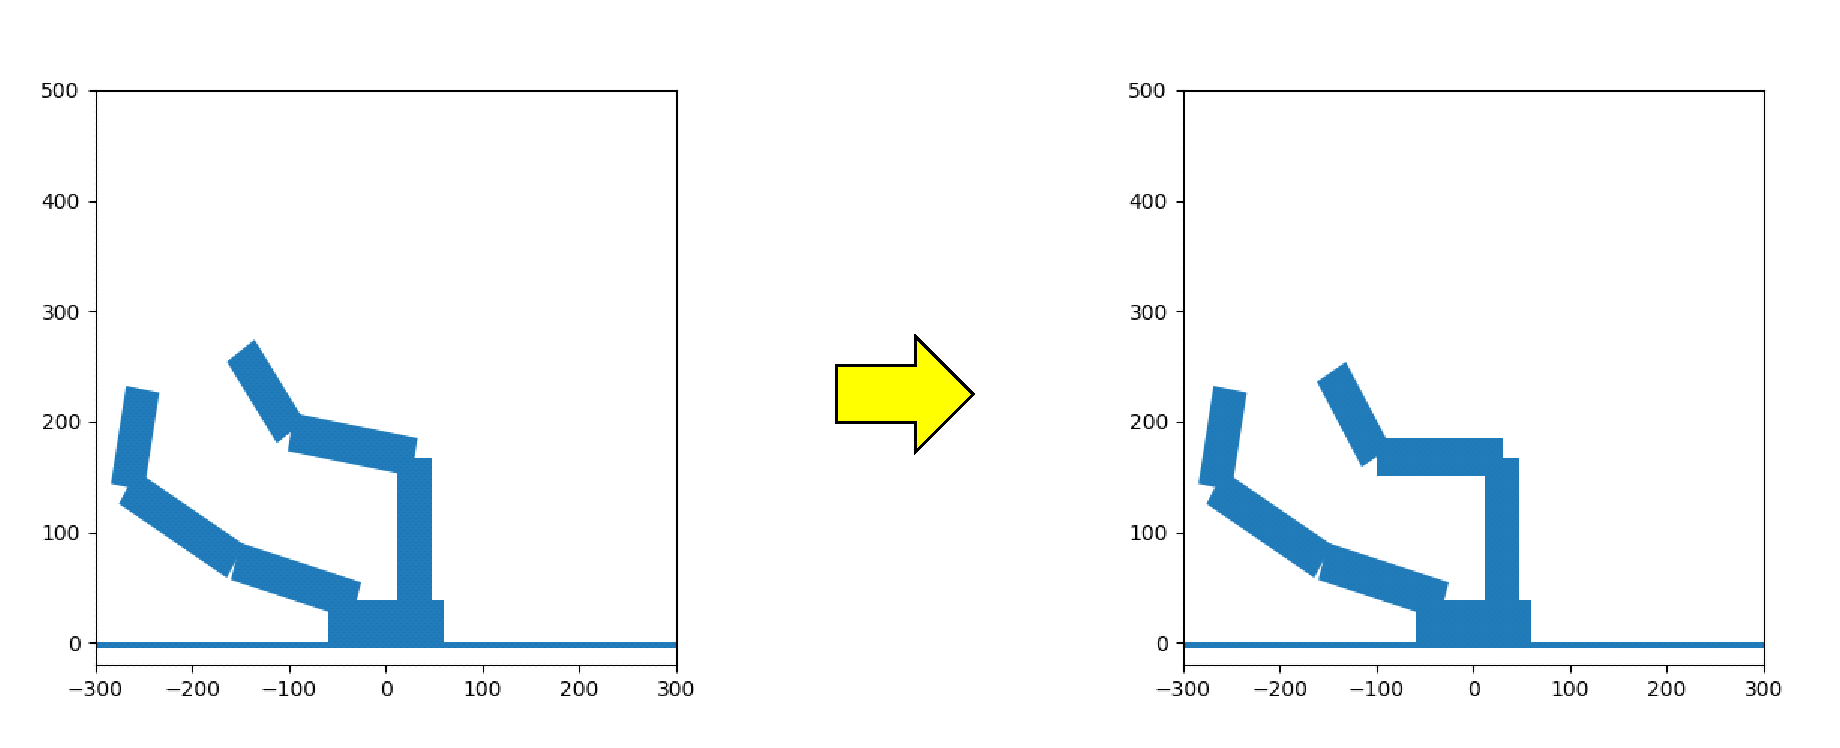
\includegraphics[width=0.8\hsize]{fig/2-sensorless-icm/cfree_obj_divided1.pdf}
    \caption{The posture of the hand when the $\mathcal{C}_{\mathrm{free\_obj}}$ is divided into multiple connected regions \cite{komiyama2021}}
    \label{fig::scim::divided1}

    \centering
    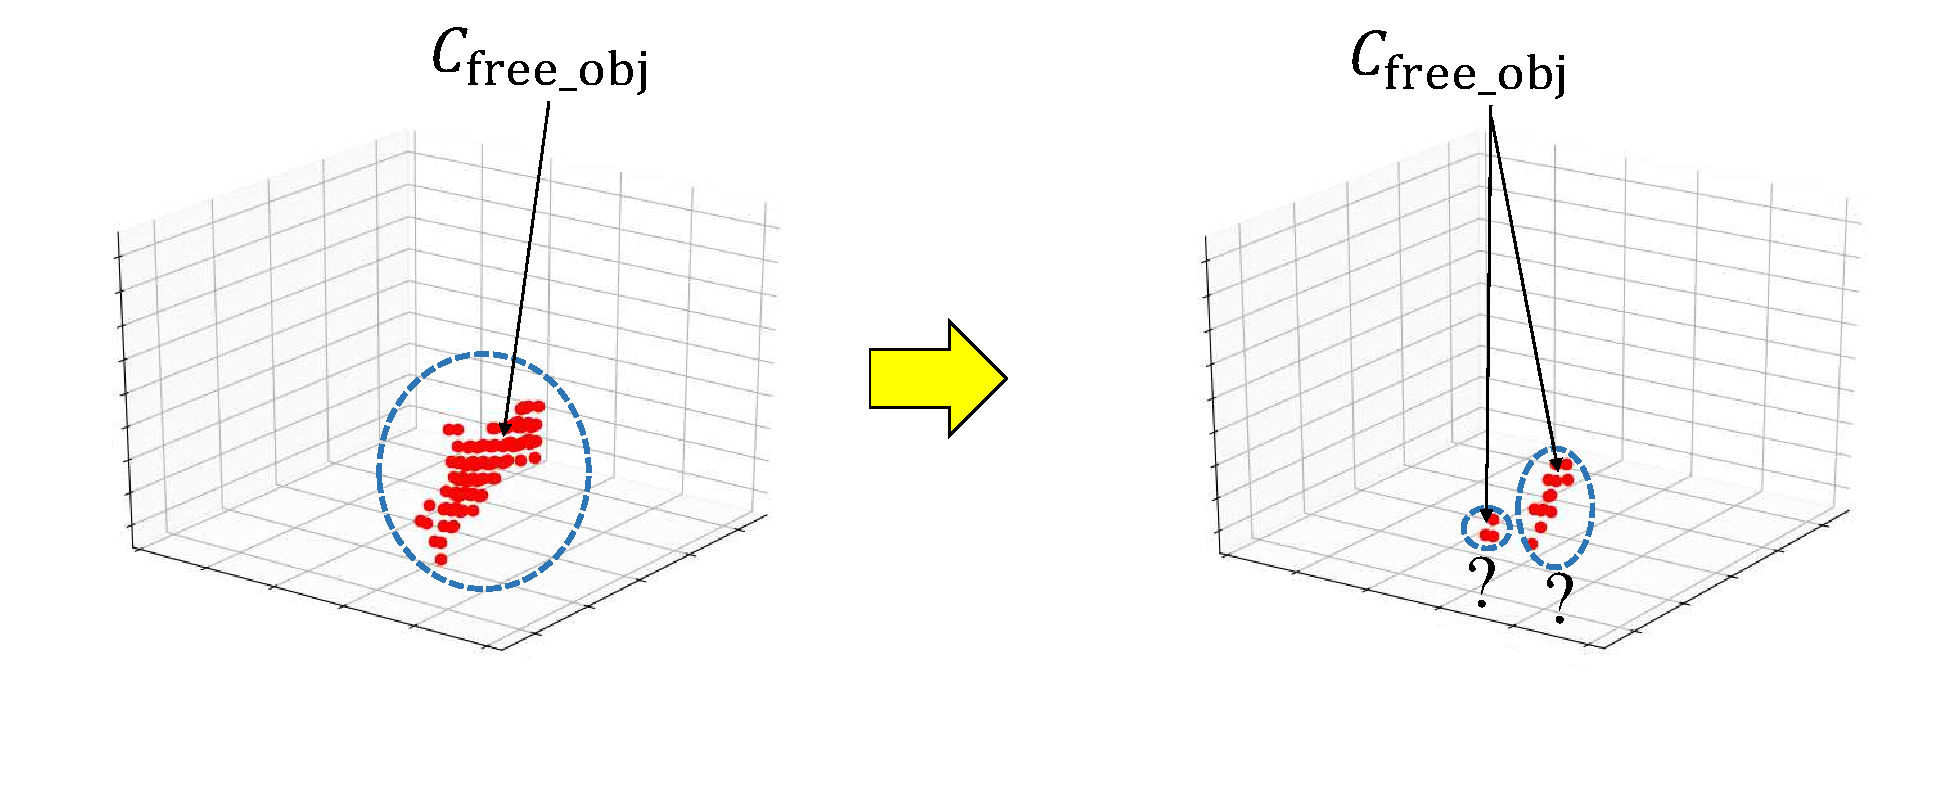
\includegraphics[width=0.85\hsize]{fig/2-sensorless-icm/cfree_obj_divided2.pdf}
    \caption{$\mathcal{C}_{\mathrm{free\_obj}}$, in the postures of the hand in \figref{fig::scim::divided1}, is divided into multiple connected regions \cite{komiyama2021}}
    \label{fig::sicm::divided2}
\end{figure}

\section{ハンドの動作計画\cite{komiyama2021}}\label{sec::sicm::planning}
先述の通り,本手法ではケージング成立条件とケージングマニピュレーション可能条件を満たした状態を維持しつつハンドを動かすことで,センサレスに対象物を目標位置・姿勢へとマニピュレーションできる.本節では,このハンドの動作生成について説明する.\cite{komiyama2021}では,経路計画手法の一つであるRRT (Rapidly-exploring Random Trees)\cite{lavalle2001}を用いた.ここで,ハンド動作はあらかじめオフラインで生成している.具体的なアルゴリズムは以下の通りである.
\begin{enumerate}
\item ハンドの初期ノード(姿勢)$\bm{q}_{\mathrm{initial}}$を設定する
\item ハンドの任意のノード$\bm{q}_{\mathrm{sample}}$をサンプリングし,$\bm{q}_{\mathrm{sample}}$から最も近いノード$\bm{q}_{\mathrm{nearest}}$を見つける\label{algo::sampling}
\item $\bm{q}_{\mathrm{nearest}}$から$\bm{q}_{\mathrm{sample}}$の方向へ長さ$\Delta l$の枝を伸ばし,そのノードを$\bm{q}_{\mathrm{new}}$とする
\item $\bm{q}_{\mathrm{new}}$において環境とハンドまたはハンド同士の干渉があれば手順\ref{algo::sampling}に戻る
\item $\bm{q}_{\mathrm{new}}$においてケージング成立条件を満たさなければ手順\ref{algo::sampling}に戻る
\item $\bm{q}_{\mathrm{new}}$においてケージングマニピュレーション可能条件を満たさなければ手順\ref{algo::sampling}に戻る
\item $\bm{q}_{\mathrm{nearest}}$から$\bm{q}_{\mathrm{new}}$へ枝を伸ばす\label{algo::fin}
\item 手順\ref{algo::sampling}から手順\ref{algo::fin}を繰り返し,$\bm{q}_{\mathrm{new}}$が終了条件を満たせば探索終了とする \label{algo::goal}
\end{enumerate}
これにより,ハンドの初期姿勢から終了姿勢までの一連の時系列データが得られる.
\begin{figure}[b]
\centering
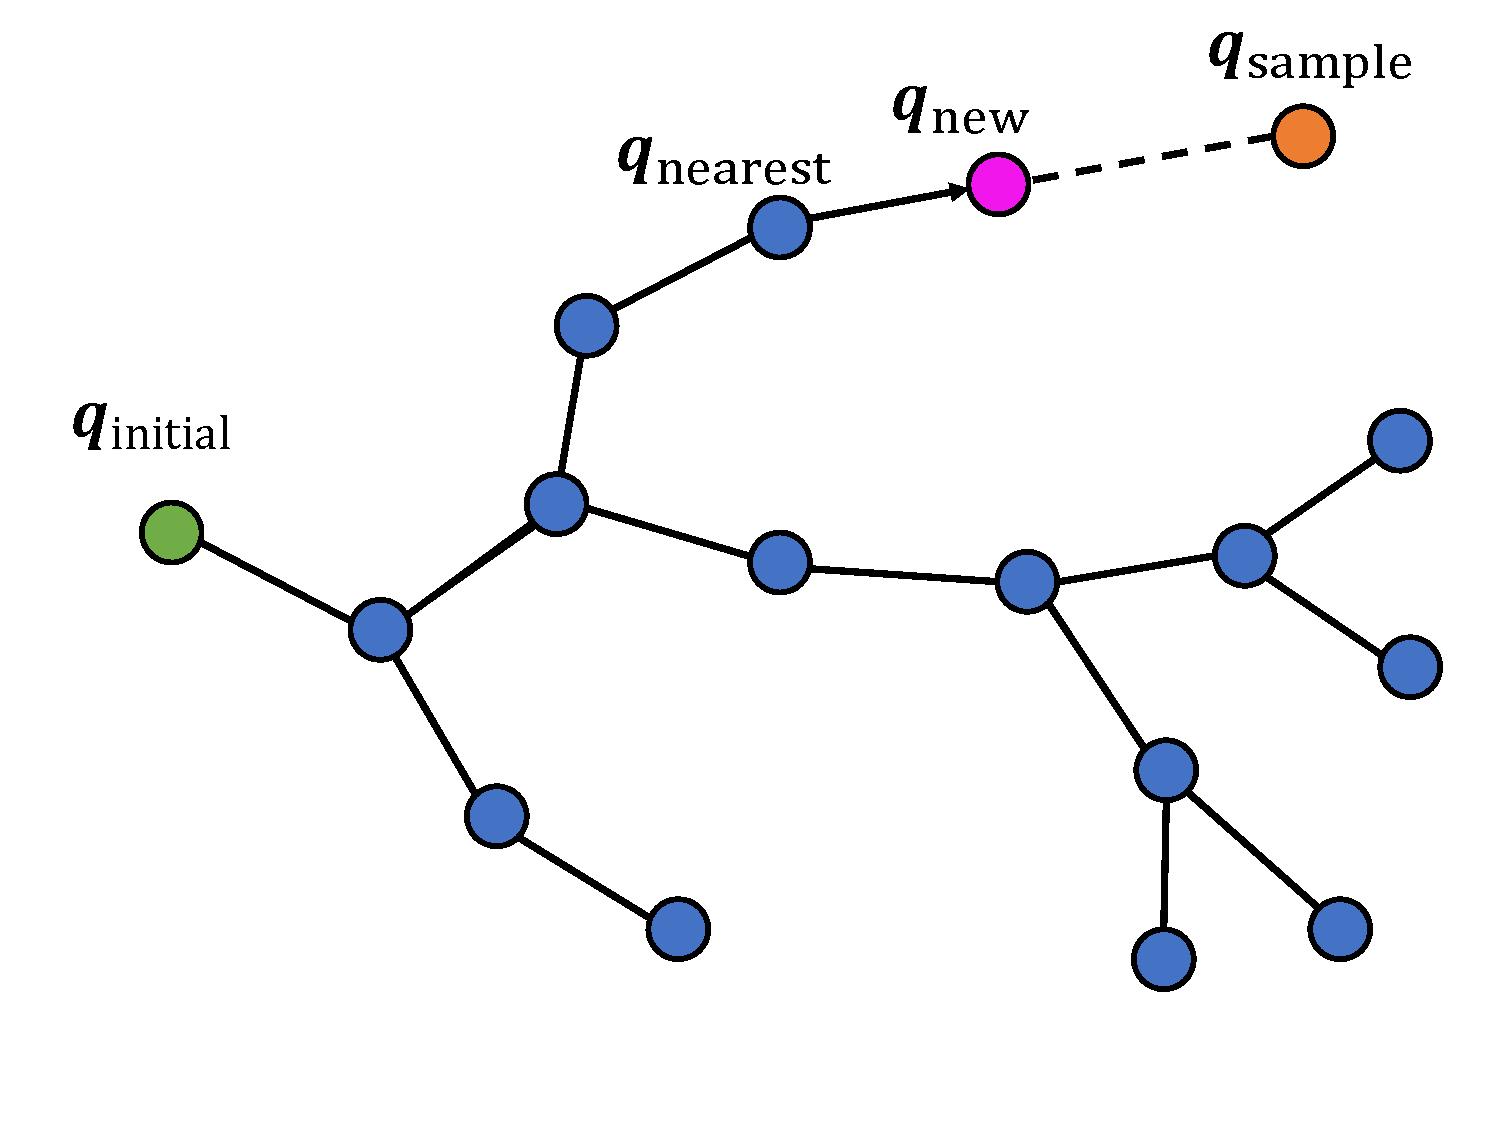
\includegraphics[width=0.5\hsize]{fig/2-sensorless-icm/rrtdiagram.pdf}
\caption{Procedure of RRT \cite{komiyama2021}}
\label{fig::sicm::rrt}
\end{figure}

手順\ref{algo::goal}の探索終了条件の説明にあたり,収束度$e$を定義する.収束度$e$は,その時のハンド姿勢によって対象物が目標位置・姿勢へどの程度,位置決めされているかを示すもので以下の\eqref{eq::sicm::e}で表される.$e$の値が小さければ小さいほど,位置決め精度が高いことを意味する.
\begin{gather}
e = \max \sqrt{(w_1(x-x_{\mathrm{goal}}))^2+(w_2(y-y_{\mathrm{goal}}))^2 + (w_3(\phi-\phi_{\mathrm{goal}}))^2}\label{eq::sicm::e} \\
(x, y, \phi) \in \mathcal{C}_{\mathrm{free\_obj}} \notag
\end{gather}
ここで,$w_1$,$w_2$,$w_3$は定数であり,これらによって\eqref{eq::sicm::e}の各項を無次元化し,位置$(x, y)$と姿勢$\phi$という異なる単位同士を一つの式で取り扱えるようにしている.\par
そして,収束度$e$と閾値$\varepsilon$を用いて探索終了条件は以下の\eqref{eq::sicm::goalcondition}となっている.
\begin{gather}
\label{eq::sicm::goalcondition}
e \leq \varepsilon 
\end{gather}
閾値$\varepsilon$を小さくする,つまり位置決め精度を高めようとすると計算時間が長くなり,閾値$\varepsilon$を大きくすると計算時間が短くなる.すなわち,位置決め精度と計算時間の間にはトレードオフの関係があり,両者のバランスを取ったパラメータ設定が重要となる.

% 白魔術
\expandafter\ifx\csname ifdraft\endcsname\relax
    \end{document}
\fi

% 黒魔術
\expandafter\ifx\csname ifdraft\endcsname\relax
    \documentclass[a4paper,twoside,12pt,papersize, dvipdfmx]{iirthesis}
    \usepackage{amsmath,amssymb,amsthm}
    \usepackage{graphicx}
    \usepackage{subcaption}
    \usepackage{url}
    \usepackage{otf}
    \usepackage{minitoc}
    \usepackage{bm}
    \usepackage{amsmath,amssymb}
    \usepackage{algorithmic}
    \usepackage{algorithm}
    \begin{document}

    \newcommand{\figref}[1]{\figurename\ref{#1}}
    \newcommand{\tabref}[1]{\tablename\ref{#1}}
    \renewcommand{\eqref}[1]{式~(\ref{#1})}
    \newcommand{\chapref}[1]{\ref{#1}章}
    \newcommand{\secref}[1]{\ref{#1}節}
    \newcommand{\ssecref}[1]{\ref{#1}項}
    \newcommand{\appref}[1]{付録\ref{#1}}
    \newcommand{\algoref}[1]{Algorithm.\ref{#1}}
\fi

\newcommand{\tab}[0]{\;\;\;\;}

\chapter{ハンド動作計画の性能向上と新アルゴリズム}\label{chap::planner}
\minitoc

\section{はじめに}\label{sec::planner::intro}
%ハンドの寸法とかPCの性能の話,閾値,コンフィギュレーションの離散粗さ,動作計画で使ってる情報の説明
本章ではハンドの動作計画における先行研究からの改善点や新たな手法の提案を説明する.本節では,実際の動作計画に使用する設定情報についてまとめる.\par

\paragraph{ハンドの設定}
まずは,ハンドの設定についてである.ハンドは\ssecref{subsec::sicm::oppositehand}の対向型ハンドを以降の全ての動作計画に対して使用している.ハンドの寸法は以下のように設定した(\figref{fig::planner::handsize}).
\begin{gather}
\notag
\left\{
\begin{aligned}
L &= 60 \mathrm{[mm]} & w& = 35 \mathrm{[mm]} & h &= 415 \mathrm{[mm]}\\
d_0 &= 38 \mathrm{[mm]} & d_1 &= 130 \mathrm{[mm]} & d_2 &= 130 \mathrm{[mm]} & d_3 = 90 \mathrm{[mm]}
\end{aligned}
\right .
\end{gather}
ハンドの姿勢は,各関節角度$\theta_i$の集合$\bm {\theta}$により決定する.$\theta_i$は,この関節に連結している2リンクの内,根元側のリンクのリンク長方向を$0^\circ$とした時の手先側リンクのリンク長方向の角度と定義している.ここで,根元側リンクから見て,反時計回りを正としている.根元の関節に関しては,鉛直方向を$0^\circ$として定めている.
\begin{figure}[b]
\centering
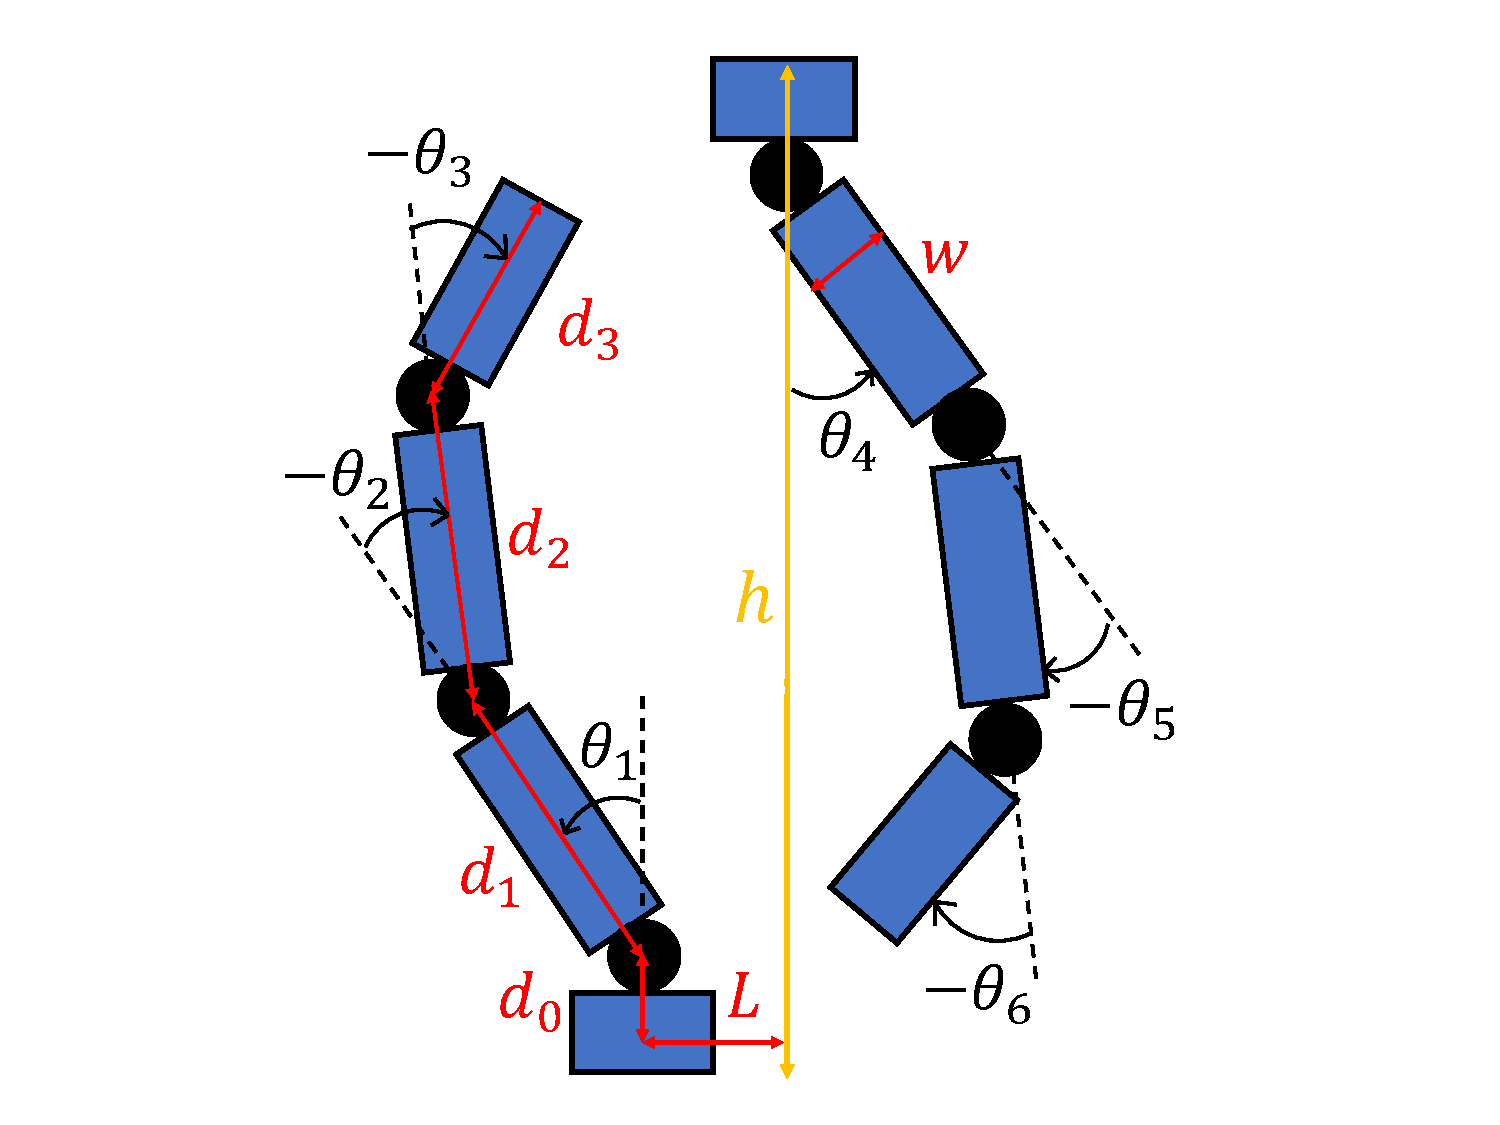
\includegraphics[width=0.7\hsize]{fig/3-new-planner/handsize.pdf}
\caption{Robot hand configuration}\label{fig::planner::handsize}
\end{figure}

\paragraph{対象物のコンフィギュレーション空間の設定}
対象物コンフィギュレーション空間は$-400 \mathrm{[mm]} \leq x \leq 400 \mathrm{[mm]}$,$-50 \mathrm{[mm]} \leq y \leq 550 \mathrm{[mm]}$,$0 \mathrm{[deg]} \leq \phi \leq 360 \mathrm{[deg]}$の直方体空間と設定した.$(x,y)$の原点は\figref{fig::planner::handsize}の原点$O$に相当し,$\phi$の原点は以下に記す対象物の姿勢$0^\circ$に相当する.前述の通り,コンフィギュレーション空間は格子状に分割し,離散的に取り扱っている.この格子点幅は$(\Delta x, \Delta y, \Delta \phi) = (10 \mathrm{[mm]}, 10 \mathrm{[mm]}, 5 \mathrm{[deg]})$と設定した.$\mathcal{P}_{\mathrm {far}}$は,ハンドから十分に離れた点群であり,以下の式で表される点群と設定した.なお,$C_{\mathrm {space}}$はコンフィギュレーション空間の全離散点群を表す.
\begin{gather}
\notag
\mathcal{P}_{\mathrm {far}} = \{ (x, y, \phi) \in C_{\mathrm {space}} \,|\, x = -400 \mathrm{[mm]} \lor x = 400 \mathrm{[mm]} \}
\end{gather}

\paragraph{対象物の形状情報}
本論文では,長方形物体,三角形物体,L字型物体,T字型物体を対象に動作計画を行った.これらの対象物の寸法情報や姿勢の定義について述べる.長方形物体は\figref{fig::planner::recdef}のように設定した.代表点は対角線の交点であり,姿勢は短辺が水平方向となるように置いた状態を$0^\circ$とした傾き角度となる.三角形物体は\figref{fig::planner::tridef}のように設定した.図心は外接円の中心であり,姿勢は$e_1$が水平方向となるように置いた状態を$0^\circ$とした傾き角度である.そのため,ユーザは三角形物体の形状情報を設定するとき,どの辺が$e_1$かを把握し,そのうえで目標姿勢を与える必要がある.L字型物体は\figref{}のように設定した.図心は\figref{fig::planner::lshapedef}のように補助線を引いて得られる長方形の対角線交点である.姿勢は文字「L」を$0^\circ$とした傾き角度である.T字型物体は\figref{fig::planner::tshapedef}のように設定した.図心,姿勢ともにL字型と同様である.なお,傾きは$0 \mathrm{[deg]} \leq \phi \leq 360 \mathrm{[deg]}$で表し,時計回りに測る.

\paragraph{PCのスペック}
OS:Ubuntu 22.04.1 LTS,CPU:AMD Ryzen 7 3700X 8-Core Processor,クロック周波数:4.43[GHz],RAM:32.0[GB]のPCで計算する.

\begin{figure}[b]
\centering
\begin{minipage}{0.49\hsize}
\centering
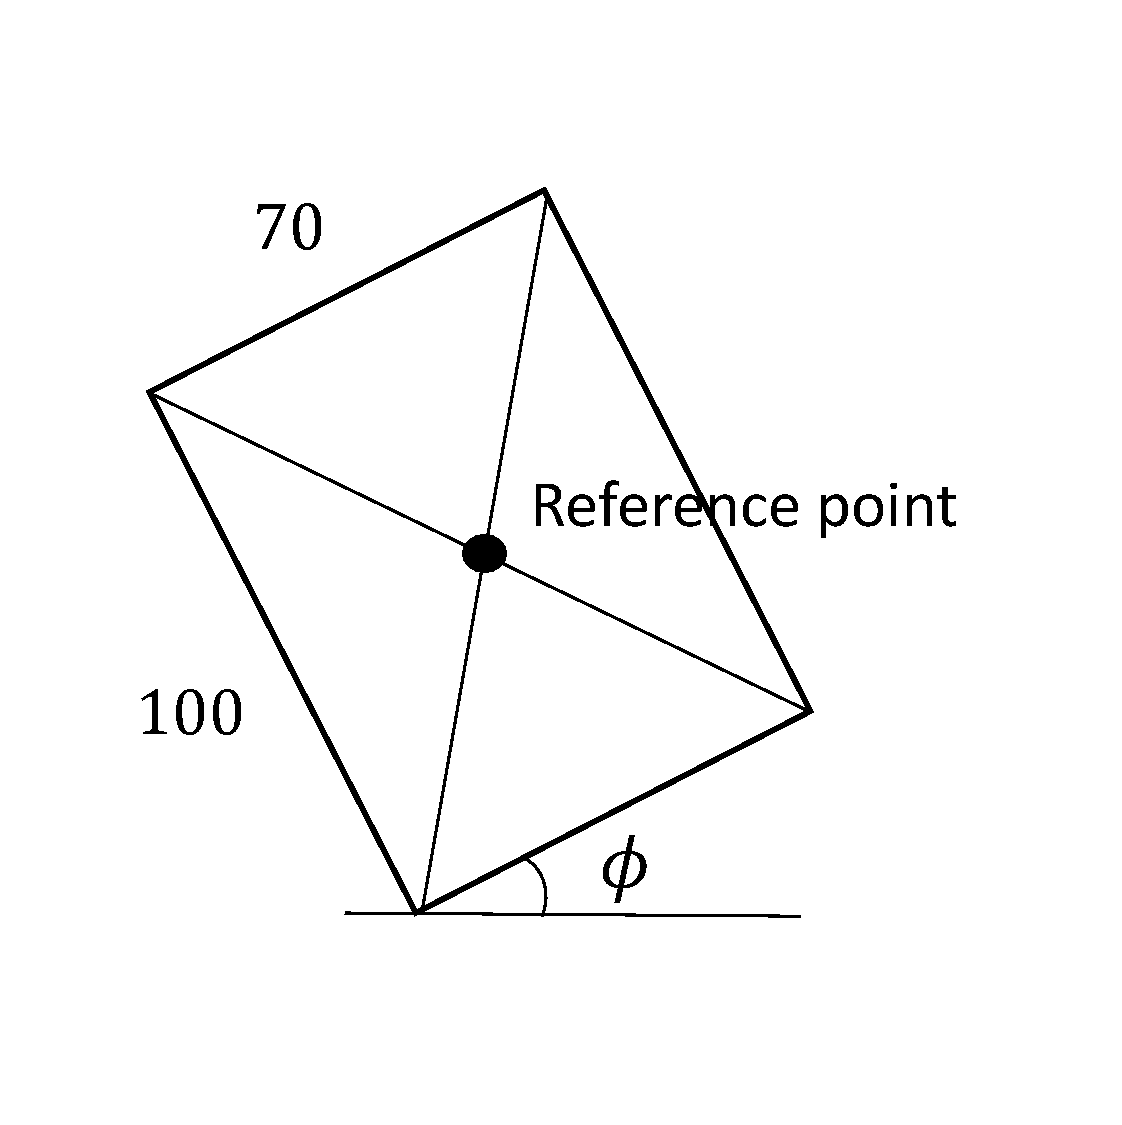
\includegraphics[width=0.9\hsize]{fig/3-new-planner/RectangleDef.pdf}
\caption{The definition of rectangle object}\label{fig::planner::recdef}
\end{minipage}\hfill
\begin{minipage}{0.49\hsize}
\centering
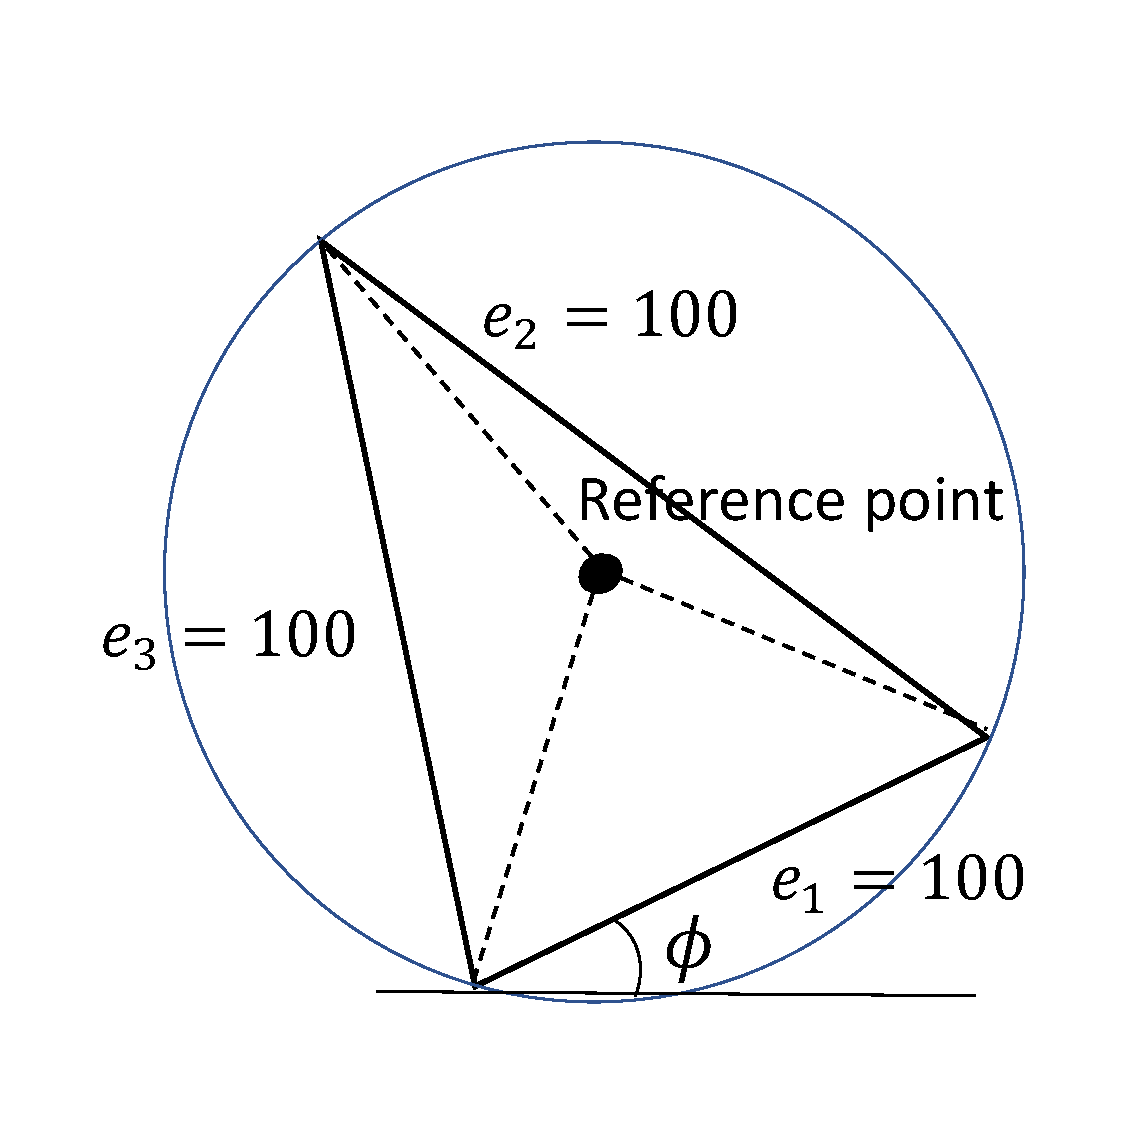
\includegraphics[width=0.9\hsize]{fig/3-new-planner/TriangleDef.pdf}
\caption{The definition of triangle object}\label{fig::planner::tridef}
\end{minipage}\hfill
\begin{minipage}{0.49\hsize}
\centering
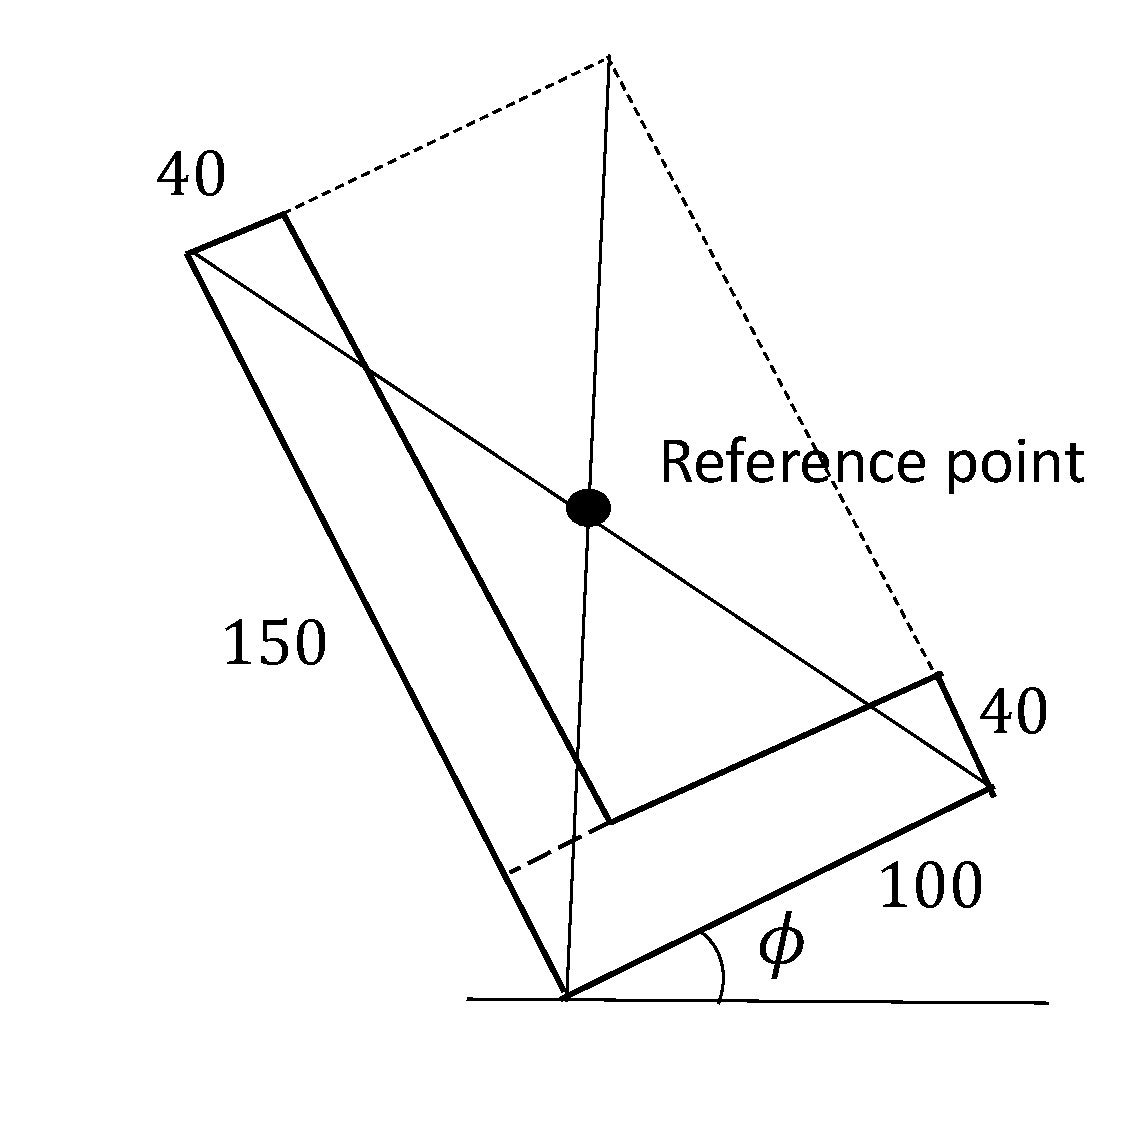
\includegraphics[width=0.9\hsize]{fig/3-new-planner/LShapeDef.pdf}
\caption{The definition of L-Shape object}\label{fig::planner::lshapedef}
\end{minipage}\hfill
\begin{minipage}{0.49\hsize}
\centering
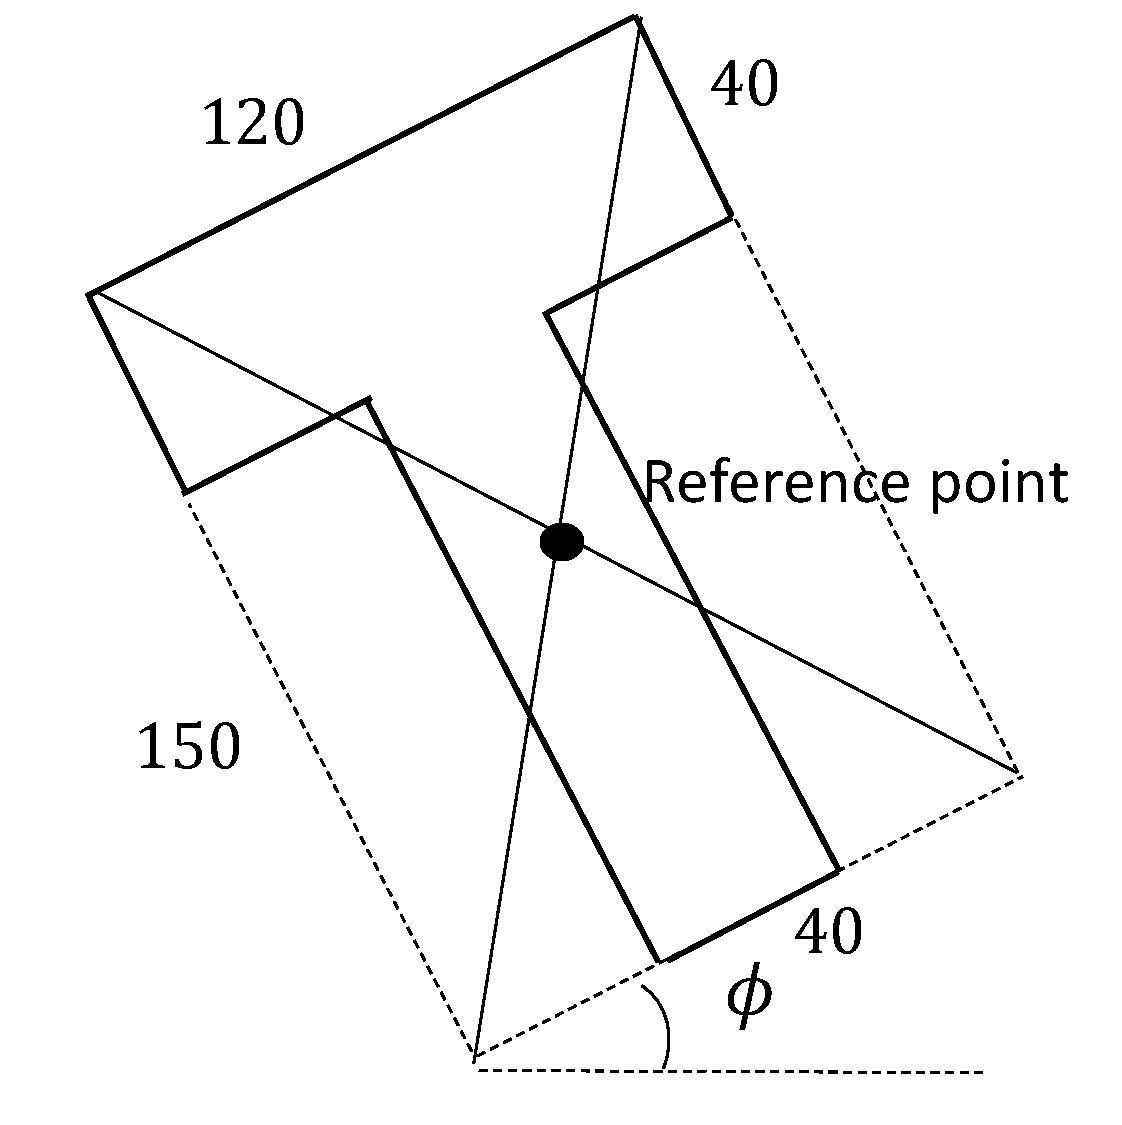
\includegraphics[width=0.9\hsize]{fig/3-new-planner/TShapeDef.pdf}
\caption{The definition of T-Shape object}\label{fig::planner::tshapedef}
\end{minipage}
\end{figure}

\section{順探索アルゴリズム}\label{sec::planner::straight}
改めて\chapref{chap::sicm}のハンド動作計画の流れを振り返る.まず,入力はハンドの初期姿勢と対象物の形状情報,そして対象物の目標位置・姿勢である.これらを基に,ハンド初期姿勢からRRTによりランダムにサンプリングし,その都度対象物の形状情報から$\mathcal{C}_{\mathrm{free\_obj}}$を計算する.ケージング成立条件,ケージングマニピュレーション可能条件の満足を確認しつつ探索を進め,対象物の目標位置・姿勢から決まる探索終了条件を満たせば動作計画が完了する.出力としては,ハンドの関節角度の時系列データが得られる.\par
この動作計画アルゴリズムを順探索アルゴリズムと呼ぶこととする.この順探索アルゴリズムには,計算時間が遅い,位置決め精度が悪いという2つの課題がある.以下の項は,これらの解決方法についてであり,前者の課題に対しては,\ssecref{subsec::planner::goalcond},\ssecref{subsec::planner::dfs}で,後者の課題に対しては,\ssecref{subsec::planner::formclosure}で説明する.

\subsection{探索終了条件の緩和}\label{subsec::planner::goalcond}
\secref{sec::sicm::planning}の通り,先行研究では対象物の目標位置・姿勢として$P_G (x_{\mathrm {goal}}, y_{\mathrm {goal}}, \phi_{\mathrm {goal}})$のコンフィギュレーション空間の1点を指定していた.しかし,本手法はパーツフィーダへの応用を想定しており,この際対象物を整列後,ベルトコンベアに乗せて生産ライン方向である$x$方向へ流す.そのため,$x$方向への目標設定は必須ではない.そこで,対象物の目標位置・姿勢を$P_G (x_{\mathrm {any}}, y_{\mathrm {goal}}, \phi_{\mathrm {goal}})$と$y$,$\phi$のみを指定するようにした.\par
これに従って,収束度$e$の定義を\eqref{eq::planner::e},探索終了条件を\eqref{eq::planner::goalcondition}のように変更した.
\begin{gather}
e = \max \sqrt{(w_1\Delta x)^2 + (w_2(y-y_{\mathrm{goal}}))^2 + (w_3(\phi-\phi_{\mathrm{goal}}))^2} \label{eq::planner::e} \\
e \leq \varepsilon \label{eq::planner::goalcondition} \\
\because  \Delta x = \dfrac{\max x  - \min x}{2} ,\;\; (x, y, \phi) \in \mathcal{C}_{\mathrm{free\_obj}} \notag
\end{gather}
これにより,$x$方向に関しては座標の調整が必要なくなったため,先行研究より早い探索終了が見込める.

\subsubsection{計算時間の比較}
\eqref{eq::planner::e}の収束度$e$の定数$w_1$,$w_2$,$w_3$を次のように設定した.
\begin{gather}
\notag
w_1=1 \mathrm{[mm^{-1}]} \tab w_2=1 \mathrm{[mm^{-1}]} \tab w_3=1 \mathrm{[deg^{-1}]}
\end{gather}
以降の収束度$e$の計算にもこれらの値を用いる.


\subsection{$\mathcal{C}_{\mathrm{free\_obj}}$の効率的な抽出}\label{subsec::planner::dfs}
\cite{komiyama2021}では$\mathcal{C}_{\mathrm{free\_obj}}$の抽出にあたって以下のような方法が取られていた.
\begin{enumerate}
\item 対象物のコンフィギュレーション空間の離散点群を全走査し,$\mathcal{C}_{\mathrm{free}}$を取り出す \label{planner::fullscan}
\item DBSCAN法\cite{ester1996}により隣り合う周囲26点群を同クラスタとするクラスタリングを$\mathcal{C}_{\mathrm{free}}$に対して行う\label{planner::clustering}
\item 手順\ref{planner::clustering}のクラスタを$\mathcal{C}_{\mathrm{free\_ICS}}$と$\mathcal{C}_{\mathrm{free\_ECS}}$に分ける
\item $\mathcal{C}_{\mathrm{free\_ICS}}$の内,\eqref{eq::sicm::continuous}に基づいて$\mathcal{C}_{\mathrm{free\_obj}}$を抽出する
\end{enumerate}
対象物のコンフィギュレーション空間の離散粗さを\secref{sec::planner::intro}のように設定した場合,点群数は約33万個となる.手順\ref{planner::fullscan}では,この点群を全走査するため計算時間が長くかかり,ボトルネックとなっている.\par

そこで,\eqref{eq::sicm::continuous}の直前$(t-\Delta t)$のハンド姿勢における$\mathcal{C}_{\mathrm{free\_obj}}(t-\Delta t)$と現在$(t)$のハンド姿勢における$\mathcal{C}_{\mathrm{free\_obj}}(t)$はオーバーラップしているという性質を応用して,$\mathcal{C}_{\mathrm{free\_obj}}(t-\Delta t)$を起点として,オーバーラップしている$\mathcal{C}_{\mathrm{free\_ICS}}$を探すという手法を提案する.\par

まず,$\mathcal{C}_{\mathrm{free\_obj}}(t-\Delta t)$の任意の一点を取り出す.壁やロボットハンドとの干渉がないか確認し,干渉があった場合は別の点を取り出す.この点を起点として,周囲を探索する.このとき,\figref{fig::planner::numbering}のように周囲の26個の方向に番号を付け,\figref{fig::planner::treegraph}のような木構造を作成する.この木構造は,根が取り出した起点,葉が起点周囲の点群となっており,周囲の探索手順の全組み合わせを表している.例えば根から1,6,13と進んだ場合は,起点から1の方向の点へ移動し,そこから6の方向へ進み,さらに13の方向へ3ステップ進んだ点へ到達していることを表す.\par

この木構造を用いて,「深さ優先」のアプローチで探索を行う.
もし,探索が$P_{\mathrm {far}}$へ到達した場合,つまり探索中の領域が$\mathcal{C}_{\mathrm{free\_ECS}}$であった場合,その領域は破棄することとなる.無駄な探索を増やさないため,その領域が$P_{\mathrm {far}}$へ到達するかどうかはなるべく早く判断したい.幅優先探索のようなアプローチを取ると,起点から全方向へ同じペースで探索が進むため,$P_{\mathrm {far}}$への到達が遅くなり,無駄な探索が多くなる.そこで,深さ優先探索というアプローチを取ると,任意の方向へ一直線に進めるだけ進むため,早い段階で$\mathcal{P}_{\mathrm {far}}$へ到達することができる.\par

これらの処理後,$\mathcal{C}_{\mathrm{free\_obj}}(t-\Delta t)$の内,探索されていない点がある場合はその点を起点として上記の操作を再度繰り返す.$P_{\mathrm {far}}$へ到達しなかった領域が$\mathcal{C}_{\mathrm{free\_obj}}(t)$となる.以上のアルゴリズムをより具体的にまとめたものを\algoref{algo::planner::dfs}に示す.

\begin{figure}[t]
\centering
\begin{minipage}{0.4\hsize}
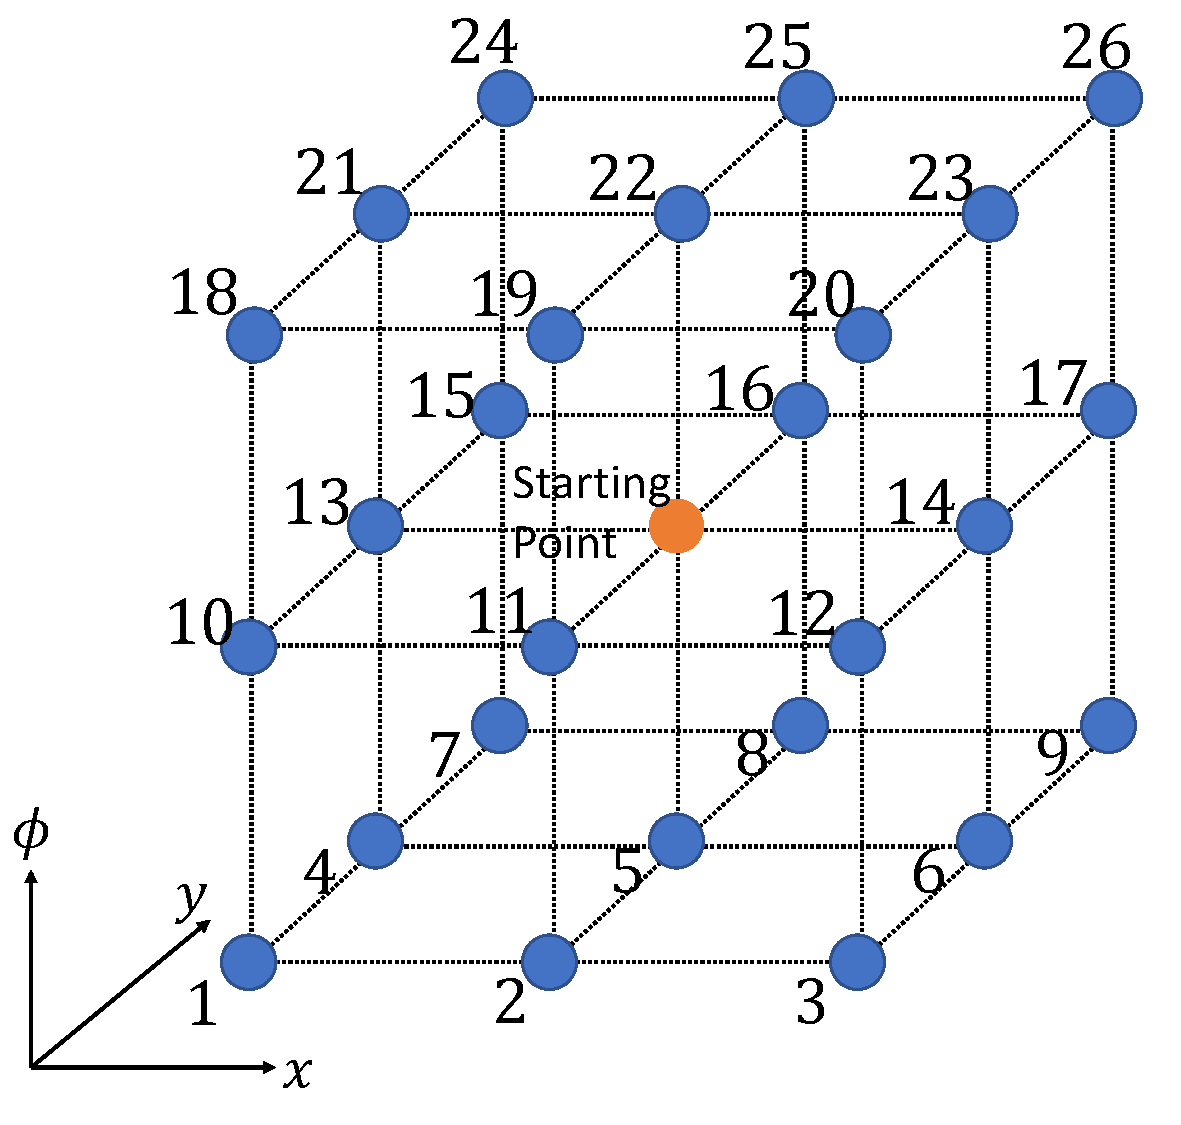
\includegraphics[width=0.9\hsize]{fig/3-new-planner/directiondef.pdf}
\caption{The definition of numbering}\label{fig::planner::numbering}
\end{minipage}\hfill
\begin{minipage}{0.59\hsize}
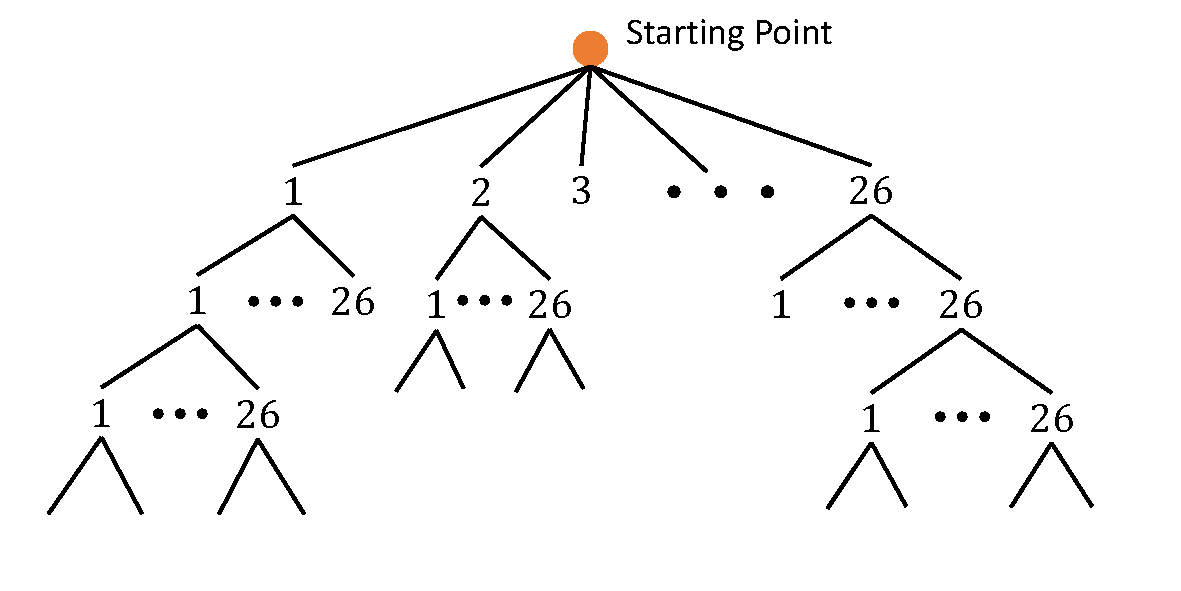
\includegraphics[width=\hsize]{fig/3-new-planner/treegraph.pdf}
\caption{Generating tree structure}\label{fig::planner::treegraph}
\end{minipage}
\end{figure}

\subsubsection{計算時間の比較}


\subsection{位置決め精度向上アルゴリズム}{\label{subsec::planner::formclosure}
計算時間の観点から,収束度$\varepsilon$は広めに設定したい.そのため,動作計画で得られたハンド最終姿勢では対象物の位置・姿勢決め精度は十分ではない.そこで,以降に示す方法によって動作計画で得られたハンド最終姿勢から微調整を加え,位置決め精度の向上を試みた.
\subsubsection{アルゴリズム}
本アルゴリズムでは,動作計画により得られた最終姿勢から更に狭まる方向へ,更にケージングが強まる方向へ微調整する.そのため,この微調整中はケージング成立条件,ケージングマニピュレーション可能条件の両者が成立していると考え,本アルゴリズムではこれを前提としている.以下,具体的なアルゴリズムについて述べる.\par
まず,対象物を目標位置・姿勢$P_G (x_{\mathrm m}, y_G, \theta_G)$に仮想的に配置する.ここで,$x$座標の目標位置$x_{\mathrm m}$に関して,\secref{subsec::planner::goalcond}の方法により,動作計画毎に位置決めされる対象物の$x$位置は変わる.そこで,$x_{\mathrm m}$には各々$\mathcal{C}_{\mathrm{free\_obj}}$の任意の$x$座標値を設定することとする.次に,片ハンドずつ対象物への距離を詰めていく.具体的には,ハンドの根元側の関節から手先側の関節の順で狭めていき,各々いずれかのハンドが対象物や他方ハンドと接触する直前で止める.この操作により,対象物の動ける範囲はさらに縮小され,位置・姿勢決め精度が向上する.\par
上記の片ハンドずつ対象物への距離を詰めていくという部分に関して,本アルゴリズムでは,左ハンド,右ハンドの順で狭めるパターンと右ハンド,左ハンドの順で狭めるパターンの2パターンを試みる.そして,より位置・姿勢決め精度が向上した方を最終的なハンド姿勢として採用する.

\subsubsection{結果}
本アルゴリズムを用いて,どの程度位置決め精度が向上するかを評価する.評価には\eqref{eq::planner::e}の収束度$e$を用い,小さいほどゴールへの収束度が高く,位置・姿勢決め精度が向上したと判断する.
\figref{fig::planner::fc}のように,$\varepsilon$の値はアルゴリズム適用前が48.8だったのに対し,右ハンド,左ハンドの順の場合は25.5で,左ハンド,右ハンドの順で狭める場合は19.6となった.これらより,位置・姿勢決め精度の向上を確認できた.
また,上記の2パターンの狭め方を試したことに関して,多くは同じ結果が得られるが,今回の場合のように精度に差が出る場合があることがあり,複数パターンを試すことの有効性が確認できた.今後,他の狭め方もパターンに含めることで更なる精度向上が望める可能性がある. \par
課題点としては,今回用いたハンドの関節角上限が$90^{\circ}$であるため,\figref{fig::planner::afterfclr},\figref{fig::planner::afterfcrl}の左ハンドの手先リンクのように,対象物まで狭めきれない場合がある.実機を改良して$90^{\circ}$以上回転を可能にすることで,更なる精度向上が望める.
\begin{figure}[b]
\centering
\begin{minipage}{0.33\hsize}
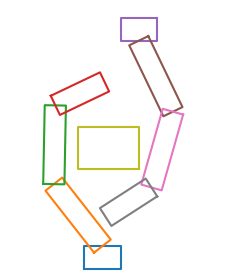
\includegraphics[width=0.9\hsize]{fig/3-new-planner/rec_before_FC.png}
\subcaption{Before applying}\label{fig::planner::beforefc}
\end{minipage}\hfill
\begin{minipage}{0.33\hsize}
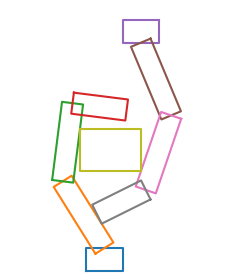
\includegraphics[width=0.9\hsize]{fig/3-new-planner/rec_FC_left_right.png}
\subcaption{left$\rightarrow$right}\label{fig::planner::afterfclr}
\end{minipage}\hfill
\begin{minipage}{0.33\hsize}
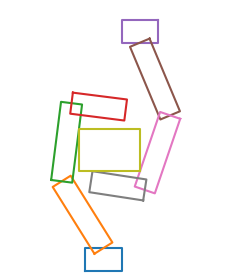
\includegraphics[width=0.9\hsize]{fig/3-new-planner/rec_FC_right_left.png}
\subcaption{right$\rightarrow$left}\label{fig::planner::afterfcrl}
\end{minipage}
\caption{The result of applying hand closing algorithm}\label{fig::planner::fc}
\end{figure}

\section{逆探索アルゴリズム}\label{sec::planner::reverse}
\subsection{RRTを用いた逆探索アルゴリズム}
順探索アルゴリズムとは逆方向のアプローチを試みる.つまり,対象物が目標位置・姿勢で位置決めされた時のハンド姿勢$\bm{\theta_G}$を探索の開始点として与え,マニピュレーションの初期状態$(t=0)$へと遡る方向へ探索することを考える.探索アルゴリズムにはRRTを用い,基本的には\ssecref{subsec::sicm::planning}と同様で,ランダムサンプリング,ケージングに関する2条件の確認,ノードの追加を行っていき,探索終了条件を満たせば動作計画を終了する.

\subsubsection{ケージング成立条件とケージングマニピュレーション可能条件}\label{subsec::planner::revcm}
ケージング成立条件に関しては順探索アルゴリズムと同様である.ケージングマニピュレーション可能条件も条件自体は,\secref{sec::sicm::caging}と変わらない.ただ,時間が逆行した方向への探索であるため処理が異なる.処理は\figref{fig::planner::cm}のような3パターンに大別できる.ただし,実際の$\mathcal{C}_{\mathrm{free\_obj}}$領域は3次元であるが,\figref{fig::planner::cm}では簡単のため2次元としてモデル化している.\figref{fig::planner::cm1}は$C_{\mathrm{free\_obj}}(t)$に対してオーバーラップしている$C_{\mathrm{free\_obj}}(t-\Delta t)$が複数ある場合である.ここでケージングマニピュレーション可能条件は,時間$t-\Delta t$における物体の存在領域$\mathcal{C}_{\mathrm{free\_obj}}(t-\Delta t)$がどの領域に遷移したかを追跡するためにオーバーラップする$\mathcal{C}_{\mathrm{free\_obj}}(t)$の領域数を1つに絞るといったものであった.この観点で\figref{fig::planner::cm1}を見ると,各々の$C_{\mathrm{free\_obj}}(t-\Delta t)$から$C_{\mathrm{free\_obj}}(t)$の1領域のみとオーバーラップしており各々追跡可能なので,ケージングマニピュレーション可能条件を満たしているといえる.この判定は,逆探索アルゴリズムでは$C_{\mathrm{free\_obj}}$が複数個存在しうることを意味している.これを踏まえて,ケージングマニピュレーション可能条件をより正確に以下のように再定義する.
\begin{itemize}
\item $C_{\mathrm{free\_obj}}(t-\Delta t)$の各々の領域は$C_{\mathrm{free\_obj}}(t)$の任意の1つの領域のみとオーバーラップする
\end{itemize}

\figref{fig::planner::cm2}の状況も発生しうる.これは,$C_{\mathrm{free\_obj}}(t-\Delta t)$に対してオーバーラップしている$C_{\mathrm{free\_obj}}(t)$が複数あるので,ケージングマニピュレーション可能条件を満たしていない.\figref{fig::planner::cm3}では,そもそもオーバーラップがないので不成立である.以上の3つで全ての場合に対して判定することができる.

\begin{figure}[b]
\begin{minipage}{0.33\hsize}
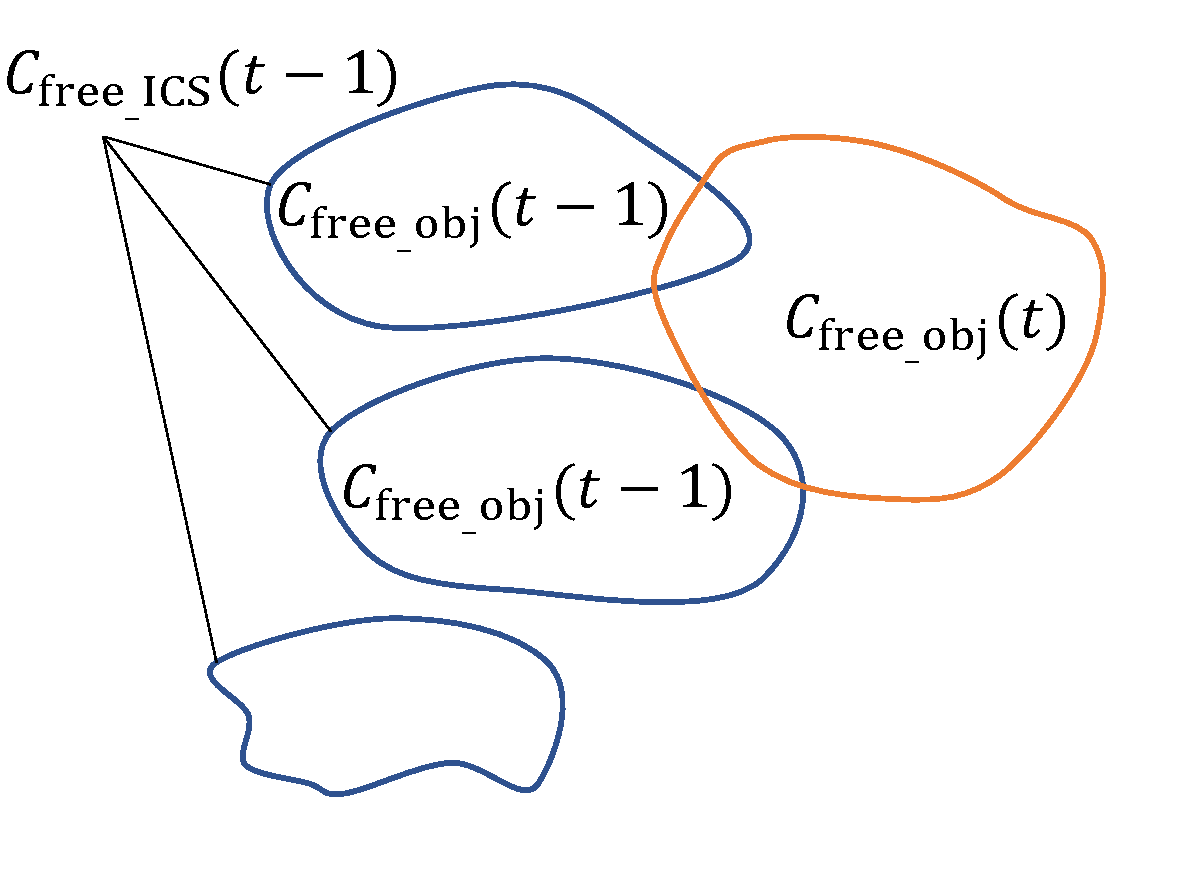
\includegraphics[width=\hsize]{fig/3-new-planner/rev_cagingmani_ver1.pdf}
\subcaption{}\label{fig::planner::cm1}
\end{minipage}\hfill
\begin{minipage}{0.33\hsize}
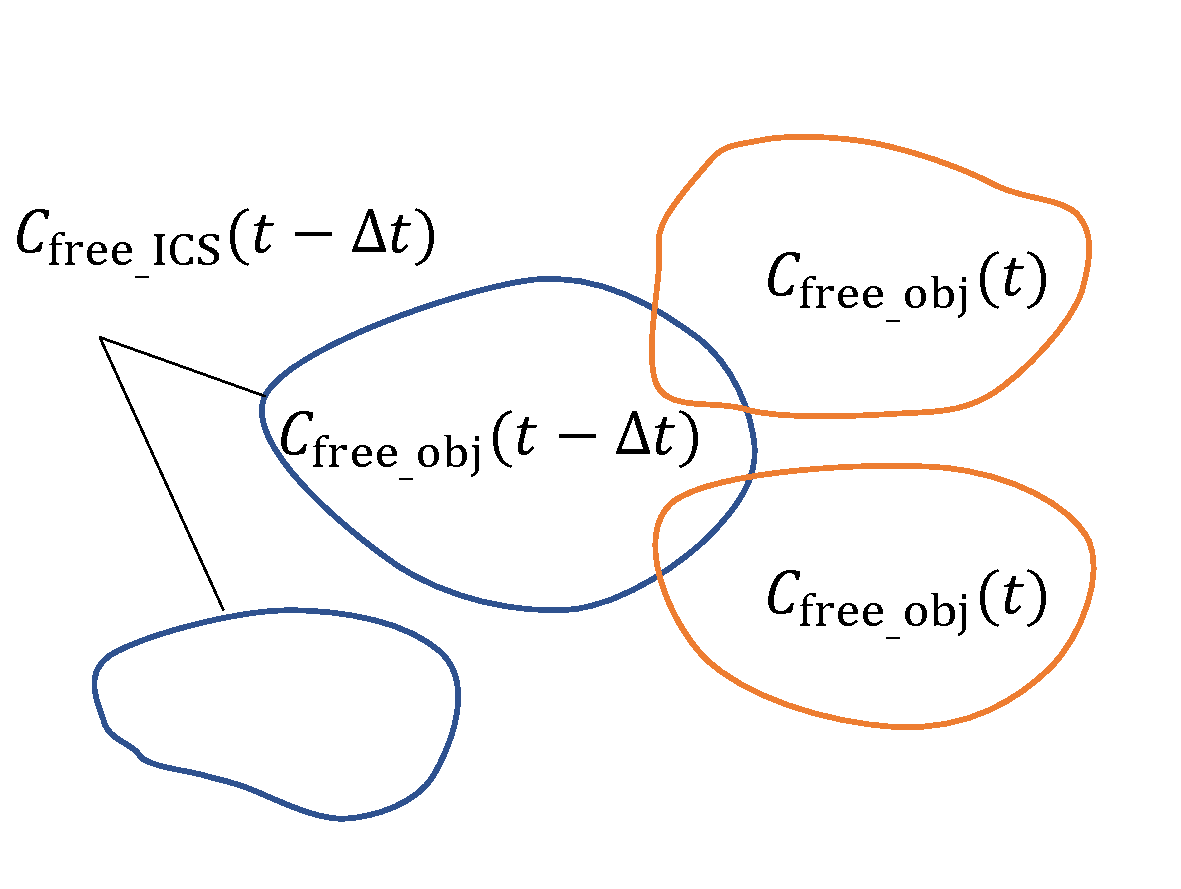
\includegraphics[width=\hsize]{fig/3-new-planner/rev_cagingmani_ver2.pdf}
\subcaption{}\label{fig::planner::cm2}
\end{minipage}\hfill
\begin{minipage}{0.33\hsize}
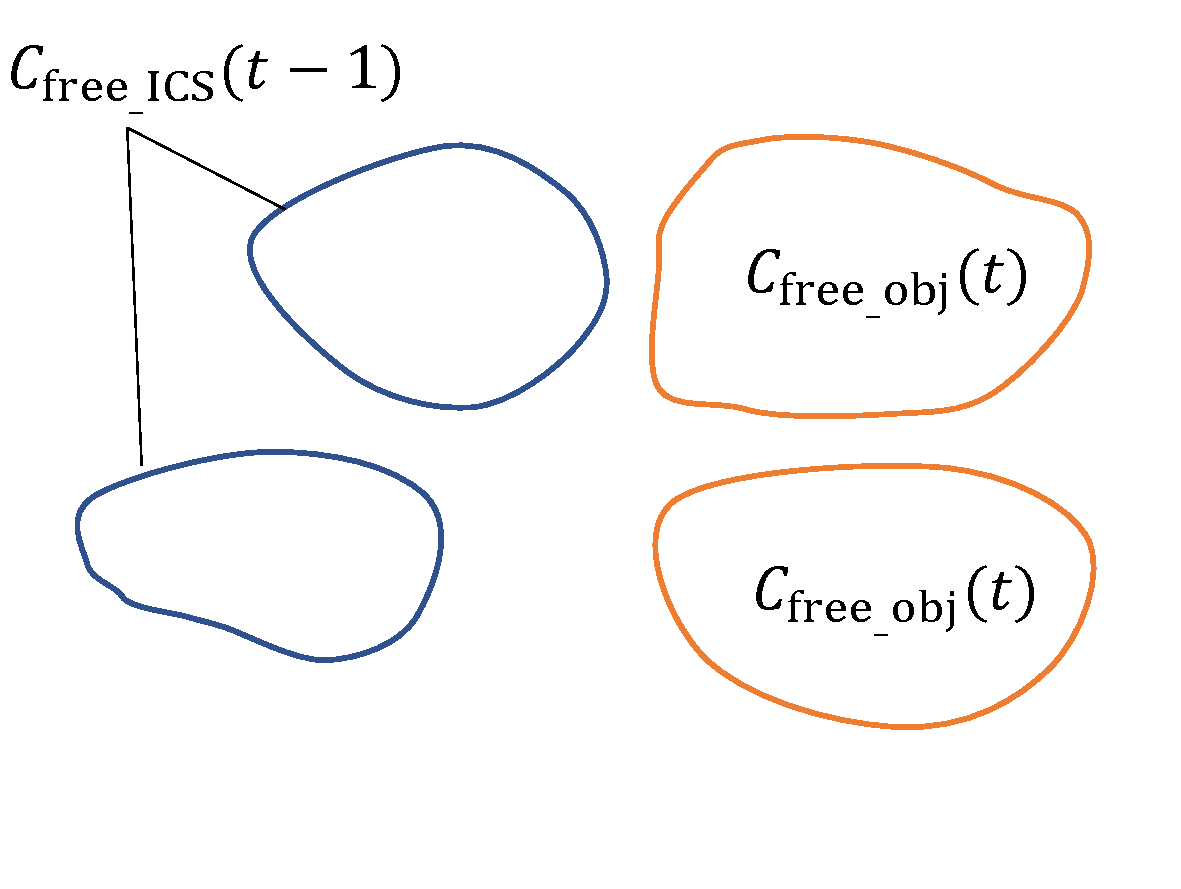
\includegraphics[width=\hsize]{fig/3-new-planner/rev_cagingmani_ver3.pdf}
\subcaption{}\label{fig::planner::cm3}
\end{minipage}
\caption{The patterns of the condition for caging manipulability for reverse exploring}
\label{fig::planner::cm}
\end{figure}

\subsubsection{逆探索アルゴリズムにおける$C_{\mathrm{free\_obj}}$の抽出}
逆探索アルゴリズムの$C_{\mathrm{free\_obj}}$抽出も\ssecref{subsec::planner::dfs}の考え方を基に実装する.まず,$t+\Delta t$における$C_{\mathrm{free\_obj}}(t+\Delta t)$の任意の点を起点として,深さ優先探索で$C_{\mathrm{free\_obj}}(t)$を抽出する.次に,$C_{\mathrm{free\_obj}}(t+\Delta t)$と$C_{\mathrm{free\_obj}}(t)$のオーバーラップを前項を基に考える.ここで,本実装では\ssecref{subsec::planner::dfs}の方法により,$C_{\mathrm{free\_obj}}$のみを抽出するようにしている.しかし通常,$C_{\mathrm{free\_obj}}$の周囲には別領域の$C_{\mathrm{free\_ICS}}$が存在している.したがって,$C_{\mathrm{free\_obj}}(t)$と$C_{\mathrm{free\_ICS}}(t+\Delta t)\, \ni C_{\mathrm{free\_obj}}(t+\Delta t)$のオーバーラップを考える必要がある.\par
そこで,$C_{\mathrm{free\_obj}}(t)$を起点として,再度$t+\Delta t$のハンド姿勢に対して\ssecref{subsec::planner::dfs}の方法で$C'_{\mathrm{free\_obj}}(t+\Delta t)$を抽出する.この$C'_{\mathrm{free\_obj}}(t+\Delta t)$の領域が0個もしくは複数個ある場合,ケージングマニピュレーション可能条件を満たさないので,$C_{\mathrm{free\_obj}}(t)$は妥当ではないと判定する.以上の処理を\algoref{algo::revdfs}にまとめる.

\subsubsection{探索終了条件}
逆探索であるため,探索の終了状態はマニピュレーションの初期状態に相当する.マニピュレーションの初期状態に求められることとしては,なるべく多様な対象物位置・姿勢を取り扱えるということが挙げられる.そこで,探索の終了条件を,物体が取りうる姿勢群を表す$\mathcal{C}_{\mathrm{free\_obj}}$のサイズが閾値$\nu$以上になった時と定めた.ここで,$\mathcal{C}_{\mathrm{free\_obj}}$のサイズは,$\mathcal{C}_{\mathrm{free\_obj}}$を構成する離散点群の数と定義している.\par
順探索アルゴリズムでは,ランダム探索なので対象物の目標位置・姿勢$P_G$から離れる方向へも探索が進むことがある.逆探索アルゴリズムでは探索の終了条件に座標の指定がなく,ただ$\mathcal{C}_{\mathrm{free\_obj}}$の領域を広げればよい.そのため,順探索のような無駄な探索方向が少なくっており,探索効率の改善が見込める.


\subsection{位置決め最適姿勢生成アルゴリズム}

\subsection{探索結果}\label{subsec::planner::revresult}
順探索アルゴリズムと計算時間の比較を行いたいが,問題設定が異なるため直接比較することはできない.そこで,繰り返し回数に対する$C_{\mathrm{free\_obj}}$のサイズの推移を紹介し,その結果をもとに簡易的に順探索アルゴリズムと比較する.以下のようなタスクを設定し,5回探索を行ったときの結果を\figref{fig::planner::revrrtres}に示す.なお,本来は探索終了閾値$\nu$を設定するが,今回は500000回の繰り返し計算を行うと終了するように設定した.
\begin{gather}
\notag
\left\{
\begin{aligned}
&ハンド初期姿勢:[\theta_1, \theta_2, \theta_3, \theta_4, \theta_5, \theta_6,] = [12, -15, -25, 5, 30, -90]\mathrm{[deg]}\\
&探索終了閾値:繰り返し計算数が500000回に到達\\
&対象物:\mathrm{L}字形物体
\end{aligned}
\right .
\end{gather}

順探索アルゴリズムでL字形物体の動作計画を行う時,入力するハンド初期姿勢$C_{\mathrm{free\_obj}}$のサイズは1000程度であることが多い.そこで,\figref{fig::planner::revrrtres}において1000に到達した時の繰り返し計算回数に注目することで簡易的に比較できる.5回の平均を取ると,繰り返し回数が~の時に$C_{\mathrm{free\_obj}}$のサイズが1000に到達している.逆探索アルゴリズムでは,繰り返し計算1回にかかる時間は約10[ms]なので,~[s]と算出される.順探索アルゴリズムと比較すると,計算時間は短くなっているといえる.


\section{両側探索アルゴリズム}\label{sec::planner::connect}
更なる計算速度の向上を目指して,順探索アルゴリズムと逆探索アルゴリズムを組み合わせた両探索アルゴリズムを提案する.
\subsection{RRT-Connectを用いた両側探索アルゴリズム}
RRT-Connect \cite{kuffner2000}を用いて両側探索アルゴリズムを構築する.これは,順探索アルゴリズムにおける探索初期状態$\bm {\theta}_S$と逆探索アルゴリズムにおける探索初期状態$\bm {\theta}_G$から交互に枝を伸ばしていき,これらの枝が連結した時,その連結経路を解として探索を終了するアルゴリズムである.なお,本アルゴリズムでは順探索アルゴリズム,逆探索アルゴリズムの探索終了条件も残しており,合計3つの探索終了条件の内,いずれかを満たせば終了するようになっている.具体的なアルゴリズムは以下のようになっている(\figref{}).
\begin{enumerate}
\item 順探索におけるハンドの初期ノード(姿勢)$\bm{q}_{\mathrm {init}}$と逆探索におけるハンドの初期ノード$\bm{q}_{\mathrm {goal}}$を設定する.以降,$\bm{q}_{\mathrm {init}}$を起点としたグラフを$T_{\mathrm {forward}}$,$\bm{q}_{\mathrm {goal}}$を起点としたグラフを$T_{\mathrm {reverse}}$とする
\item ハンドの任意のノード$\bm{q}_{\mathrm {sample}}$をサンプリングし,$T_{\mathrm {forward}}$の内,$\bm{q}_{\mathrm{sample}}$から最も近いノード$\bm{q}_{\mathrm{nearest}}$を見つける\label{algo::planner::sampling}
\item $\bm{q}_{\mathrm{nearest}}$から$\bm{q}_{\mathrm{sample}}$の方向へ長さ$\Delta l$の枝を伸ばし,そのノードを$\bm{q}_{\mathrm{new}}$とする \ref{algo::planner::qnew}
\item $\bm{q}_{\mathrm{new}}$において環境とハンドまたはハンド同士の干渉,ケージングに関する2条件を判定し,妥当でなければ手順\ref{algo::planner::sampling}に戻る
\item $\bm{q}_{\mathrm{new}}$と一番近いノード$\bm{q}_{\mathrm{opposite\_near}}$を$T_{\mathrm {reverse}}$から探索する\label{algo::planner::biasbegin}
\item $\bm{q}_{\mathrm{opposite\_near}}$から$\bm{q}_{\mathrm{new}}$に向けて長さ$\Delta l$の枝を伸ばし,$\bm{q}_{\mathrm{opposite\_new}}$とする\label{algo::planner::proceed}
\item $\bm{q}_{\mathrm{opposite\_new}}$において環境とハンドまたはハンド同士の干渉,ケージングに関する2条件を判定する
\item $\bm{q}_{\mathrm{opposite\_new}}$が妥当かつ探索終了条件を満たさない場合,$\bm{q}_{\mathrm{opposite\_new}}$を$\bm{q}_{\mathrm{opposite\_near}}$とし,手順\ref{algo::planner::proceed}に戻る\label{algo::planner::biasend}
\item $\bm{q}_{\mathrm{opposite\_new}}$が妥当でない場合,役割を入れ替えて(詳細は後述する),手順\ref{algo::planner::sampling}に戻る \label{algo::planner::change}
\item $\bm{q}_{\mathrm{opposite\_new}}$が探索終了条件を満たせば終了\label{algo::planner::goalcond}
\end{enumerate}

手順\ref{algo::planner::change}の役割を入れ替えるという部分は具体的には以下のことを行う.
\begin{itemize}
\item 手順\ref{algo::planner::sampling}の$T_{\mathrm {forward}}$と$T_{\mathrm {reverse}}$を入れ替える
\item 手順\ref{algo::planner::biasbegin}の$T_{\mathrm {reverse}}$と$T_{\mathrm {forward}}$を入れ替える
\end{itemize}


本アルゴリズムの特徴は三つある.一つ目は,探索終了条件を3つ設定していることである.それぞれ,$T_{\mathrm {forward}}$が順探索アルゴリズムの探索終了条件を満たす,$T_{\mathrm {reverse}}$が逆探索アルゴリズムの探索終了条件を満たす,$T_{\mathrm {forward}}$と$T_{\mathrm {reverse}}$が繋がり,結合点間のケージング2条件も満たす,の3つとなっている.いずれかを満たせばよいため,順探索アルゴリズム,逆探索アルゴリズムと比べて条件は緩くなっていると言える.二つ目は,手順\ref{algo::planner::biasbegin}から\ref{algo::planner::biasend}にかけて非常に強いバイアスがかかるという点である.スタートからゴール方向へ,ゴールからスタート方向へ進めるだけ進めるというバイアスがかかっているため,順探索アルゴリズムや逆探索アルゴリズムのようなランダムサンプリングに比べて効率的な探索になっている.三つ目は,経路が比較的滑らかなことである.順探索アルゴリズム,逆探索アルゴリズムではランダムに枝を伸ばしていくため,凹凸の多い経路が生成される.このような経路では,マニピュレーションにかかる時間が増加したり,関節部にかかる負荷が大きくなったりといったことが考えられる.一方,本探索手法では手順\ref{algo::planner::proceed}において一直線に枝を伸ばすような探索が行われるので,順探索アルゴリズム,逆探索アルゴリズムに比べて滑らかな経路が生成される.

\subsection{計算時間の比較}
両側探索アルゴリズムは,順探索アルゴリズムにマニピュレーション終了状態のハンド姿勢を,逆探索アルゴリズムにマニピュレーション初期状態のハンド姿勢を追加で与え,これら追加情報を活用して探索を効率化するアルゴリズムである.この追加情報によって順探索アルゴリズム,逆探索アルゴリズムそれぞれからどの程度,計算速度が速くなるかを検証する.\par
\subsubsection*{順探索アルゴリズムと両側探索アルゴリズムの比較}
\begin{gather}
\notag
\left\{
\begin{aligned}
&ハンド初期姿勢:[\theta_1, \theta_2, \theta_3, \theta_4, \theta_5, \theta_6,] = [40, -50, -30, 40, -50, -30]\mathrm{[deg]}\\
&ハンド最終姿勢:[\theta_1, \theta_2, \theta_3, \theta_4, \theta_5, \theta_6,] = [12, -15, -25, 5, 30, -90]\mathrm{[deg]}\\
&対象物:\mathrm{L}字形物体\\
&対象物の目標位置・姿勢:[x_{\mathrm {goal}}, y_{\mathrm {goal}}, \phi_{\mathrm {goal}}] = [{\mathrm {any}}, 200 \mathrm{[mm]}, 0 \mathrm{[deg]}]\\
&順探索の終了閾値:\varepsilon = 50\\
&逆探索の終了閾値:\nu = 1000
\end{aligned}
\right .
\end{gather}
20回動作計画を行い,計算時間を計測した.結果は\tabref{tab::planner::LFB}のようになった.
\begin{table}[bt]
    \centering
    \caption{Comparison of calculation time between forward search and bidirectional search}
    \label{tab::planner::LFB}
    \begin{tabular}{|c|c|c|}
    \hline
        ~ & Forward search & Bidirectional search \\ \hline
        1 & 614.1 [s] & 19.5 [s] \\ \hline
        2 & 569.2 & 85.4 \\ \hline
        3 & 1097.1 & 11.0 \\ \hline
        4 & 117.3 & 19.2 \\ \hline
        5 & 285.8 & 63.5 \\ \hline
        6 & 176.9 & 26.1 \\ \hline
        7 & 457.0 & 101.1 \\ \hline
        8 & 650.1 & 12.3 \\ \hline
        9 & 1219.7 & 48.1 \\ \hline
        10 & 2341.8 & 33.3 \\ \hline
        11 & 113.7 & 12.2 \\ \hline
        12 & 2048.0 & 14.9 \\ \hline
        13 & 939.6 & 52.0 \\ \hline
        14 & 41.9 & 60.9 \\ \hline
        15 & 848.5 & 20.6 \\ \hline
        16 & 2760.0 & 22.7 \\ \hline
        17 & 2410.0 & 8.2 \\ \hline
        18 & 375.6 & 155.4 \\ \hline
        19 & 229.4 & 19.2 \\ \hline
        20 & 225.4 & 81.5 \\ \hline
        Average & 877.4 [s]  & 43.4 [s] \\ \hline
        SD & 850.1 [s] & 38.4 [s] \\ \hline
    \end{tabular}
\end{table}

2つのデータが等分散か否かを$F$検定により判断する.有意水準$5\%$とし,両側検定を行う.
\begin{gather}
\left\{
\notag
\begin{aligned}
&帰無仮説& &H_0:\sigma_1^2 = \sigma_2^2\\
&対立仮説& &H_1:\sigma_1^2 \neq \sigma_2^2\\
&検定統計量& &T = \dfrac{s_1^2}{s_2^2} = 489.6\\
&棄却域& &F(f_1, f_2; \alpha/2)=F(19, 19; 0.025) = 2.53\\
\end{aligned}
\right .
\end{gather}
$T=489.6 > 2.53$なので,$H_0$は棄却され,2つのデータは等分散ではないといえる.\par
2つのデータは非等分散なので,ウェルチの$t$検定により両側探索アルゴリズムの平均計算時間が順探索アルゴリズムに比べて有意に短いことを示す.
有意水準を$5\%$とし,両側探索を行う.
\begin{gather}
\left\{
\notag
\begin{aligned}
&帰無仮説& &H_0:\mu_1 = \mu_2\\
&対立仮説& &H_1:\mu_1 \neq \mu_2\\
&検定統計量& &T = \dfrac{\overline{x}_{1}-\overline{x}_{2}}{\sqrt{\dfrac{s_1^{2}}{n_{1}}+\dfrac{s_2^{2}}{n_{2}}}} = 4.38\\
&自由度& &f=\dfrac{1}{\dfrac{C^2}{n_1-1}+\dfrac{(1-C)^2}{n_2-1}}=19.1\simeq 19 & \because C=\dfrac{\dfrac{s_1^2}{n_1}}{\dfrac{s_1^2}{n_1}+\dfrac{s_2^2}{n_2}}\\
&棄却域& &t(f, \alpha/2) = t(19, 0.025) = 2.093
\end{aligned}
\right .
\end{gather}
$T=4.38 > 2.093$なので,$H_0$は棄却され,両側探索アルゴリズムの計算時間は順探索アルゴリズムに比べて有意に短いことが示された.


\subsubsection*{逆探索アルゴリズムと両側探索アルゴリズムの比較}
\begin{gather}
\notag
\left\{
\begin{aligned}
&ハンド初期姿勢:[\theta_1, \theta_2, \theta_3, \theta_4, \theta_5, \theta_6,] = [40, -50, -30, 40, -50, -30]\mathrm{[deg]}\\
&ハンド最終姿勢:[\theta_1, \theta_2, \theta_3, \theta_4, \theta_5, \theta_6,] = []\mathrm{[deg]}\\
&対象物:\mathrm{T}字形物体\\
&対象物の目標位置・姿勢:[x_{\mathrm {goal}}, y_{\mathrm {goal}}, \phi_{\mathrm {goal}}] = [{\mathrm {any}}, 200 \mathrm{[mm]}, 0 \mathrm{[deg]}]\\
&順探索の終了閾値:\varepsilon = 50\\
&逆探索の終了閾値:\nu = 1000
\end{aligned}
\right .
\end{gather}
20回動作計画を行い,計算時間を計測した.結果は\tabref{tab::planner::TRB}のようになった.
\begin{table}[bt]
    \centering
    \caption{Comparison of calculation time between reverse search and bidirectional search}
    \label{tab::planner::TRB}
    \begin{tabular}{|c|c|c|}
    \hline
        ~ & Reverse search & Bidirectional search \\ \hline
        1 & 44.2 [s] & 2.5 [s] \\ \hline
        2 & 3.3 & 5.5 \\ \hline
        3 & 3.6 & 3.6 \\ \hline
        4 & 14.1 & 4.4 \\ \hline
        5 & 302.6 & 3.1 \\ \hline
        6 & 119.6 & 4.1 \\ \hline
        7 & 16.3 & 2.5 \\ \hline
        8 & 22.2 & 2.1 \\ \hline
        9 & 9.07 & 3.9 \\ \hline
        10 & 11.1 & 3.2 \\ \hline
        11 & 82.6 & 3.0 \\ \hline
        12 & 59.2 & 1.8 \\ \hline
        13 & 33.5 & 2.4 \\ \hline
        14 & 43.2 & 2.2 \\ \hline
        15 & 265.3 & 2.7 \\ \hline
        16 & 223.1 & 2.8 \\ \hline
        17 & 107.7 & 3.5 \\ \hline
        18 & 3.6 & 3.2 \\ \hline
        19 & 48.4 & 2.8 \\ \hline
        20 & 33.3 & 2.4 \\ \hline
        Average & 72.3 [s]  & 3.1 [s] \\ \hline
        SD & 89.7 [s] & 0.9 [s] \\ \hline
    \end{tabular}
\end{table}
2つのデータが等分散か否かを$F$検定により判断する.有意水準$5\%$とし,両側検定を行う.
\begin{gather}
\left\{
\notag
\begin{aligned}
&帰無仮説& &H_0:\sigma_1^2 = \sigma_2^2\\
&対立仮説& &H_1:\sigma_1^2 \neq \sigma_2^2\\
&検定統計量& &T = \dfrac{s_1^2}{s_2^2} = 489.6\\
&棄却域& &F(f_1, f_2; \alpha/2)=F(19, 19; 0.025) = 2.53\\
\end{aligned}
\right .
\end{gather}
$T=489.6 > 2.53$なので,$H_0$は棄却され,2つのデータは等分散ではないといえる.\par
2つのデータは非等分散なので,ウェルチの$t$検定により両側探索アルゴリズムの平均計算時間が順探索アルゴリズムに比べて有意に短いことを示す.
有意水準を$5\%$とし,両側探索を行う.
\begin{gather}
\left\{
\notag
\begin{aligned}
&帰無仮説& &H_0:\mu_1 = \mu_2\\
&対立仮説& &H_1:\mu_1 \neq \mu_2\\
&検定統計量& &T = \dfrac{\overline{x}_{1}-\overline{x}_{2}}{\sqrt{\dfrac{s_1^{2}}{n_{1}}+\dfrac{s_2^{2}}{n_{2}}}} = 4.38\\
&自由度& &f=\dfrac{1}{\dfrac{C^2}{n_1-1}+\dfrac{(1-C)^2}{n_2-1}}=19.1\simeq 19 & \because C=\dfrac{\dfrac{s_1^2}{n_1}}{\dfrac{s_1^2}{n_1}+\dfrac{s_2^2}{n_2}}\\
&棄却域& &t(f, \alpha/2) = t(19, 0.025) = 2.093
\end{aligned}
\right .
\end{gather}
$T=4.38 > 2.093$なので,$H_0$は棄却され,両側探索アルゴリズムの計算時間は順探索アルゴリズムに比べて有意に短いことが示された.

\section{各アルゴリズムの利点・欠点}
以上,順探索アルゴリズム,逆探索アルゴリズム,両側探索アルゴリズムの3つを紹介した.いずれのアルゴリズムの利点と欠点があり,ニーズに応じてこれらのアルゴリズムを使い分けることが望ましい.本節では,各アルゴリズムの利点・欠点とどのような場合にどのアルゴリズムが便利かについて述べる.\par

まず,順探索アルゴリズムについてである.このアルゴリズムの利点は,対象物の目標位置・姿勢$P_{G} (x_{G}, y_{G}, \phi_{G})$の入力から,そこに位置決めできるハンド姿勢が生成される点にある.対象物形状が複雑になると,目標位置・姿勢$P_G$へ位置決めできるハンド姿勢を手動で見つけるのは困難な場合がある.このような場合,順探索アルゴリズムでは収束度$e$という位置決めの評価指標を用いて位置決めに適切なハンド姿勢を探索でき,有用である.欠点は,前述の通り計算時間が遅いことである.逆探索アルゴリズムとは厳密に比較できないが概ね遅くなっており,両側探索アルゴリズムと比べると明らかに遅かった.また,初期姿勢を与えるのが困難,手間であるという点も挙げられる.任意に初期姿勢を与えた場合,その姿勢がケージングを満たしているか,様々な対象物位置・姿勢を取り扱えるかを確かめる必要がある.加えて,与えた初期姿勢によっては目標位置・姿勢までの経路が存在しない,またはそのような経路を見つけるのが困難な場合があり,慎重にハンド初期姿勢を与える必要がある.\par

次に,逆探索アルゴリズムについてである.このアルゴリズムの利点は,指定が難しいハンド初期姿勢を自動で生成できる点である.ハンドの初期姿勢は上述のような条件を満たす必要があり,ユーザが任意に与えるのは困難,手間である.そのため,「対象物の取りうる位置・姿勢群数が閾値以上」という条件を与えて探索し,これを満たし次第,ハンドの初期姿勢を得ることができる逆探索アルゴリズムは利便性が高い.また,対象物を位置決めできるハンド姿勢を与えるという点もメリットになる場合がある.上述の通り,このようなハンド姿勢を与えるのは困難な場合もあるが,対象物形状がシンプルな場合,人間の方が即座に適した姿勢を見つけることができる場合がある.この場合,逆探索アルゴリズムだと,ハンドは最適な姿勢へ推移していくことが保証され,かつ指定が難しい初期姿勢も計算で自動的に算出してくれるため,有用なものとなっている.欠点としては,順探索アルゴリズムと同様,与えた位置決め姿勢から初期姿勢までの経路が存在しない,またはそのような経路を見つけるのが困難な場合があるということが挙げられる.また,人間が与えた位置決め姿勢はある程度適した姿勢だと思われるが,最適である保証がないという点に注意する必要がある.\par

最後に,両側探索アルゴリズムについてである.利点は計算時間が最も短い点である.\secref{sec::planner::connect}の通り,順探索アルゴリズム,逆探索アルゴリズムに比べて計算時間が有意に短いことが示されており,有用性が高くなっている.二つ目の利点は,経路生成の成功率が高い点である.順探索アルゴリズム,逆探索アルゴリズムの共通の欠点として,与える情報によっては経路が存在しない,またはそのような経路を見つけるのが困難な場合があることを述べた.これに対して,両側探索アルゴリズムでは3つの探索終了条件を設定しているため,いずれかの入力情報が不適切でも経路が生成される可能性が残っている.例えば与えたマニピュレーション初期姿勢が適切ではなく,目標位置・姿勢までの経路が存在しない場合,つまり順探索方向に経路が存在しない場合でも,逆探索方向で経路が生成されうる.また,順探索アルゴリズムや逆探索アルゴリズムのようなランダム探索において,経路を見つけるのが非常に困難な場合でも,両側探索アルゴリズムの強力なバイアスによって経路を見つけやすくなっていると考えられる.欠点としては,与える情報がマニピュレーション初期姿勢,対象物位置決め姿勢など,上記アルゴリズム2つに比べて多いことが挙げられる.対象物が複雑形状で,与える姿勢の検討がつかない場合,両側探索アルゴリズムを適用するのは困難になる.\par

これらを踏まえて,どのようなシチュエーションにどのアルゴリズムが適しているかを考える.
まず,任意対象物を本システムでマニピュレーションするのが初めてなどの理由で,どのようなハンド位置決め姿勢が適しているか等の知見がなく,また人間が与えるのも困難な場合,順探索アルゴリズムを用いるのが望ましい.最初は,なるべく多様な位置・姿勢群を扱えるというようなことは考えず,ひとまずケージングを満たしている初期姿勢を与える.これに対して,順探索アルゴリズムで動作計画を行うことで,ハンド位置決め姿勢を得ることができる.\par
次に,任意対象物を位置決めできる姿勢が容易に準備できる,または上記のタスクによってハンド位置決め姿勢を得ている前提で,なるべく多様な位置・姿勢群を扱えるようなマニピュレーション初期姿勢を探索したい場合,逆探索アルゴリズムを用いるのが望ましい.探索終了条件に関して,\secref{sec::planner::reverse}のように$\mathcal{C}_{\mathrm{free\_obj}}$のサイズが閾値$\nu$以上になった時というような設定でも良いが,\ssecref{subsec::planner::revresult}のように繰り返し回数(時間)で与えることもできる.これは,例えば限られた短い時間で可能な限り扱える位置・姿勢群を増やすといった用途に役立つ設定となっている.このように探索終了条件においてもニーズに応じた設定が可能である.\par
最後に,任意対象物をマニピュレーションするにあたって,ある程度の知見があり動作計画にかかる時間を重視する場合,両側探索アルゴリズムが適している.他には,経路を見つけやすいという観点から順探索アルゴリズムや逆探索アルゴリズムでは経路を見つけられないような厳しい問題設定に対して動作計画を実行するというような使い方も考えられる.例えば,順探索アルゴリズムでは不可能なくらいハンド初期姿勢における$\mathcal{C}_{\mathrm{free\_obj}}$のサイズを広くとり,ハンド位置決め姿勢への強いバイアスによって経路を見つけるといった使い方が挙げられる.別の使い道としては,すでに生成された動作の再計画が挙げられる.順探索アルゴリズムや逆探索アルゴリズムでは凹凸の多い経路が作られやすく,このような経路ではマニピュレーション時間が長くなる.一方,\secref{sec::planner::connect}で述べた通り,両側探索アルゴリズムでは比較的滑らかな経路が生成されやすい.この特徴を活かして,順探索アルゴリズムや逆探索アルゴリズムでの計画で得られた動作情報をもとに,両側探索アルゴリズムで再計画することにより,滑らかな優れた経路を生成することができる.



% 白魔術
\expandafter\ifx\csname ifdraft\endcsname\relax
    \end{document}
\fi

% 黒魔術
\expandafter\ifx\csname ifdraft\endcsname\relax
    \documentclass[a4paper,twoside,12pt,papersize, dvipdfmx]{iirthesis}
    \usepackage{amsmath,amssymb,amsthm}
    \usepackage{graphicx}
    \usepackage{subcaption}
    \usepackage{url}
    \usepackage{otf}
    \usepackage{minitoc}
    \usepackage{bm}
    \usepackage{amsmath,amssymb}
    \begin{document}

    \newcommand{\figref}[1]{\figurename\ref{#1}}
    \newcommand{\tabref}[1]{\tablename\ref{#1}}
    \renewcommand{\eqref}[1]{式~(\ref{#1})}
    \newcommand{\chapref}[1]{\ref{#1}章}
    \newcommand{\secref}[1]{\ref{#1}節}
    \newcommand{\ssecref}[1]{\ref{#1}項}
    \newcommand{\appref}[1]{付録\ref{#1}}
\fi


\chapter{多角形のセンサレスin-handケージングマニピュレーションの計画・実行}
\minitoc

\section{実験装置}
%ベルトコンベアとか3Dプリンタで作ったとかサーボモータとか

\section{長方形のマニピュレーション}
\section{三角形のマニピュレーション}
\section{L字形のマニピュレーション}
\section{T字形のマニピュレーション}
\section{考察}




% 白魔術
\expandafter\ifx\csname ifdraft\endcsname\relax
    \end{document}
\fi

% 黒魔術
\expandafter\ifx\csname ifdraft\endcsname\relax
    \documentclass[a4paper,twoside,12pt,papersize, dvipdfmx]{iirthesis}
    \usepackage{amsmath,amssymb,amsthm}
    \usepackage{graphicx}
    \usepackage{subcaption}
    \usepackage{url}
    \usepackage{otf}
    \usepackage{minitoc}
    \usepackage{bm}
    \usepackage{amsmath,amssymb}
    \usepackage{times} % times new roman
    \begin{document}
    % ベンリダナー
    \newcommand{\figref}[1]{\figurename\ref{#1}}
    \newcommand{\tabref}[1]{\tablename\ref{#1}}
    \renewcommand{\eqref}[1]{式~(\ref{#1})}
    \newcommand{\chapref}[1]{\ref{#1}章}
    \newcommand{\secref}[1]{\ref{#1}節}
    \newcommand{\ssecref}[1]{\ref{#1}項}
    \newcommand{\appref}[1]{付録\ref{#1}}
\fi

\minitoc

\chapter{結論}\label{chap::conclusion}
\section{結論}\label{sec::conclusion::conclusion}
本研究では,センサレスin-handケージングマニピュレーションの有用性を高め,パーツフィーダを実用化するために,新たなハンド構成,対向型ハンドの提案,動作計画の高性能化の2つについて取り組んだ.前者に関して,従来のハンド構成,並列型ハンドではマニピュレーションの際,ジャミングという問題が発生していた.これに対して従来研究において様々な解決法が試みられたが,依然として一定の頻度でジャミングは発生していた.また,並列型ハンドの手元付近は構造上マニピュレーションできないという問題があった.そこで,対向型ハンドの提案により,ジャミングを限りなく減らすことができ,またどこに対象物があってもマニピュレーションできるようになった.後者に関しては,まず従来法である順探索アルゴリズムの改善を行った.パーツフィーダへ応用を考慮した探索終了条件の緩和,$\mathcal{C}_{\mathrm{free\_obj}}$の効率的な抽出により計算時間を大幅に削減した.また,動作計画より得られた最終姿勢からハンドを対象物に向けて狭めていくという手法により,位置決め精度も向上させた.次に,逆探索アルゴリズムを提案した.マニピュレーション終了時の位置決めされたハンド姿勢を探索の初期値としてユーザーが与える(,または最適姿勢生成アルゴリズムによって生成する)ことができるため,位置決め精度の高い経路が生成されることが保証されている.最後に両探索アルゴリズムを提案した.順探索アルゴリズムと逆探索アルゴリズムを組み合わせたアルゴリズムであり,マニピュレーション開始姿勢から終了姿勢へ,またその逆への非常に強いバイアスがかかるため効率の良い探索アルゴリズムとなっている.実際に計算時間の短縮が確認できた.また,順探索アルゴリズム,逆探索アルゴリズムの両方の位置決め精度向上の仕組みも引き継いでいるため,位置決め精度も同様に高くなっている.これら3つのアルゴリズムの中では,両探索アルゴリズムが計算時間,位置決め精度の面で最も優れているが,ユーザーのニーズによっては他の探索アルゴリズムが適している場合もあり,各々使い分けられるというのも本手法の有用性を高めている.\par

本動作計画で生成した経路を用いて,長方形,三角形,L字型,T字型物体に対して実機でマニピュレーションを行った.ロボットハンドには,3リンク3関節のハンドを向かい合うように2つ組み合わせた対向型ハンドを用いた.結果,いずれの対象物においても,ジャミングなく目標位置・姿勢までマニピュレーションされることを確認した.しかし,実機の誤差により計算程の位置決め精度は得られなかった.

以上,対向型ハンドの提案,動作計画の高性能化によりセンサレスin-handケージングマニピュレーションの有用性を高めることができた.これにより,ジャミングが起こらず安定し,かつ再立ち上げ時間が短く,位置決め精度が高い汎用パーツフィーダの実用化に貢献できたと考えている.

\section{今後の展望}\label{sec::conclusion::future}



% 白魔術
\expandafter\ifx\csname ifdraft\endcsname\relax
    \end{document}
\fi


\backmatter

%黒魔術
\expandafter\ifx\csname ifdraft\endcsname\relax
 \documentclass[a4paper,twoside,12pt,papersize, dvipdfmx]{iirthesis}
 \usepackage{amsmath,amssymb,amsthm}
 \usepackage{graphicx}
 \usepackage{subfig}
 \usepackage{url}
 \usepackage{otf}
 \usepackage{minitoc}
 \usepackage{bm}
 \usepackage{amsmath,amssymb}
 \usepackage{times} % times new roman
 \begin{document}
\fi

\chapter{謝辞}\label{chapter:acknowledgements}


%白魔術
\expandafter\ifx\csname ifdraft\endcsname\relax
  \end{document}
\fi

% 黒魔術
\expandafter\ifx\csname ifdraft\endcsname\relax
    \documentclass[a4paper,twoside,12pt,papersize, dvipdfmx]{iirthesis}
    \usepackage{amsmath,amssymb,amsthm}
    \usepackage{graphicx}
    \usepackage{subcaption}
    \usepackage{url}
    \usepackage{otf}
    \usepackage{minitoc}
    \usepackage{bm}
    \usepackage{amsmath,amssymb}
    \usepackage{times} % times new roman
    \begin{document}
    % ベンリダナー
    \newcommand{\figref}[1]{\figurename\ref{#1}}
    \newcommand{\tabref}[1]{\tablename\ref{#1}}
    \renewcommand{\eqref}[1]{式~(\ref{#1})}
    \newcommand{\chapref}[1]{\ref{#1}章}
    \newcommand{\secref}[1]{\ref{#1}節}
    \newcommand{\ssecref}[1]{\ref{#1}項}
    \newcommand{\appref}[1]{付録\ref{#1}}
\fi

\chapter{参考文献}\label{chap:bibliography}

\begin{thebibliography}{}
%1-intro
\bibitem[Dwivedi+ 2018]{dwivedi2018}
A. Dwivedi, Y. Kwon, A. J. McDaid and M. Liarokapis:
``EMG Based Decoding of Object Motion in Dexterous, In-Hand Manipulation Tasks,''
{\it 2018 7th IEEE International Conference on Biomedical Robotics and Biomechatronics (Biorob)},
2018, pp.~1025--1031, doi:~10.1109/BIOROB.2018.8487222.

\bibitem[Rimon+ 1999]{rimon1999} 
E. Rimon and A. Blake:
``Caging Planar Bodies by One-Parameter Two-Fingered Gripping Systems,''
{\it The International Journal of Robotics Research}, vol.~18, no.~3, pp.~299--318, 1999.

\bibitem[込山 2021]{komiyama2021}
込山 隼:
``センサレスin-hand ケージングマニピュレーションによる物体の位置・姿勢制御'',
横浜国立大学大学院理工学府, ポートフォリオ, 2021.
  
\bibitem[Hertkorn+ 2013]{hertkorn2013}


  \bibitem[Bircher+ 2019]{bircher2019}
      %Walter G. Bircher, Andrew S. Morgan, Kaiyu Hang, Aaron M. Dollar,
	W. G. Bircher, A. S. Morgan, K. Hang, A. M. Dollar,
  	``Energy Gradient-Based Graphs for Planning Within-Hand Caging Manipulation'',
  	2019.
    
      \bibitem[Chavan-Dafle+ 2020]{chavan-dafle2020}
 % 	Nikhil Chavan-Dafle, Rachel Holladay, Alberto Rodriguez,
 	N. Chavan-Dafle, R. Holladay, A. Rodriguez,
  	``Planar In-Hand Manipulation Via Motion Cones'',
  	 The International Journal of Robotics Research,
  	 Vol.~39, No.~2--3, pp.~163--182,
  	2020.
  	
    \bibitem[Ospina+ 2020]{ospina2020}
%  	Diego Ospina, Alejandro Ramirez-Serrano,
	D. Ospina, A. Ramirez-Serrano,
  	``Sensorless In-Hand Manipulation by An Underactuated Robot Hand'',
  	 ASME. J. Mechanisms Robotics. October 2020,
  	 Vol.~12, No.~5: 051009, 
  	2020.

    \bibitem[田原 2013]{tahara2013}
	田原 健二,
  	``動的安定把持に基づくマニピュレーション'',
  	 日本ロボット学会誌,
  	 Vol.~31, No.~4, pp.~364--369,
  	2013.  	

    \bibitem[田原 2020]{tahara2020}
    	田原 健二,
  	``多指ロボットハンドによる物体把持のダイナミクスと受動性'',
  	 システム/情報/制御,
  	 Vol.~64, No.~12,pp.~477--482,
  	2020. 
  	
 	\bibitem[Mannam+ 2019]{mannam2019}
  %	Pragna Mannam, Alexander Volkov, Jr., Robert Paolini, Gregory Chirikijan, Matthew T. Mason,
  	P. Mannam, A. Volkov, Jr., R. Paolini, G. Chirikijan, M. T. Mason,
  	``Sensorless Pose Determination Using Randomized Action Sequences'',
  	 Entropy, Vol.~21, No.~2, p.~154, 
  	2019.
  	
  	\bibitem[Akella+ 2000]{akella2000}
  	S. Akella, W. H. Huang, K. M. Lynch, M. T. Mason,
  	``Parts Feeding on a Conveyor with a One Joint Robot'',
  	 Algorithmica 26,
  	 pp.~313--344,
  	2000.
  	
  	\bibitem[Udhayakumar+ 2021]{udhayakumar2021}
  	S. Udhayakumar, A. Mohan, J. Gowthamachandran,  R. Prakash, P. Shanmugam,
  	``Development of Visionless Flexible Part Feeder for Handling Shock Absorbers'',
  	 Materials, Design, and Manufacturing for Sustainable Environment, Springer Singapole, 
  	 pp.~141--154,
  	2021.  	
  	
\bibitem[上久木田 2022]{kamikukita2022}
上久木田 治毅:
``センサレス in-hand ケージングマニピュレーションに基づく汎用パーツフィーダの開発'', 
横浜国立大学理工学部, 卒業論文, 2022.
  	
\bibitem[浅村 2013]{asamura2013} 
浅村 知洋:
``ロボットハンドのためのIn-hand ケージングマニピュレーション'', 
横浜国立大学大学院工学府, 修士論文, 2013.
\end{thebibliography}

% 白魔術
\expandafter\ifx\csname ifdraft\endcsname\relax
    \end{document}
\fi


%\appendix
%% 黒魔術
\expandafter\ifx\csname ifdraft\endcsname\relax
    \documentclass[a4paper,twoside,12pt,papersize, dvipdfmx]{iirthesis}
    \usepackage{amsmath,amssymb,amsthm}
    \usepackage{graphicx}
    \usepackage{subcaption}
    \usepackage{url}
    \usepackage{otf}
    \usepackage{minitoc}
    \usepackage{bm}
    \usepackage{amsmath,amssymb}
    \begin{document}
    % ベンリダナー
    \newcommand{\figref}[1]{\figurename\ref{#1}}
    \newcommand{\tabref}[1]{\tablename\ref{#1}}
    \renewcommand{\eqref}[1]{式~(\ref{#1})}
    \newcommand{\chapref}[1]{\ref{#1}章}
    \newcommand{\secref}[1]{\ref{#1}節}
    \newcommand{\ssecref}[1]{\ref{#1}項}
    \newcommand{\appref}[1]{付録\ref{#1}}
\fi

\chapter{付録}\label{chap:appendix}


% 白魔術
\expandafter\ifx\csname ifdraft\endcsname\relax
    \end{document}
\fi


\end{document}
